\chapter{Making Sense of Complex Temporal Relationship}
\label{chap:timesets}

\graphicspath{{Chapter4/figures/}}

\blfootnote{Published at the \emph{Information Visualization} journal~\cite{Nguyen2015}.}\autoref{chap:schemaline} presents a timeline visualization technique, SchemaLine, to explore the temporal relationship of sensemaking through the high-level analytic provenance manually captured by users. However, SchemaLine cannot show events belonging to multiple schemas, or \emph{sets} for generality, limiting users from exploring complex temporal relationship. In this chapter, we introduce a novel technique -- \emph{\textcb{TimeSets}} -- to address that issue. TimeSets visually groups events that belong to the same set but still preserves their temporal order. It color codes the backgrounds of the entire sets to distinguish them and uses colored gradient backgrounds for the intersections among those sets. It also addresses the scalability issue in SchemaLine by dynamically adjusting the level of detail for each event to suit the amount of information and display estate. A controlled experiment was conducted to evaluate its effectiveness by comparing it to a state-of-the-art method. The results showed significant advantage in accuracy and user preference.

\section{Introduction}
In the previous chapter, SchemaLine is shown to be effective in exploring temporal relationship of intelligence sensemaking by allowing analysts to construct narratives (or schemas) from their annotations (or events). However, it does not allow an event to be part of multiple schemas, which is common in early data exploration. Also, literature in sensemaking theory (\autoref{sub:lr-sensemaking})  suggests the same requirement. Pirolli and Card's model shows that analysts can generate multiple hypotheses from the same information they found. Data--Frame model proposes that multiple frames can be created to account for the same data. Therefore, it is critical for a timeline visualization for sensemaking to effectively show both \emph{temporal} and \emph{set} (for generality) information of events simultaneously.

Back in 1765, one of the oldest documented timelines produced by Joseph Priestley -- the Chart of Biography~\cite{Priestley1765} -- already denotes sets of elements. The timeline includes two thousand famous persons from 1200 BC to 1800 AD classified into six categories based on their most well-known achievement. The timeline is divided into six horizontal bands, one for each category, to visualize the set relations. However, it is clear that an element cannot be part of multiple sets. 

More sophisticated techniques have been designed to visualize multiple-set events. One technique is to assign set membership to a visual channel of element icons such as color hue or shape~\cite{TimeGlider2016}. However, events in the same set are not necessarily located close to each other, making it difficult to follow them chronologically or to have an overview of the distribution of events~\cite{SimileTimeline2009,TimeGlider2016}. Another common approach is to visually connect events in the same set~\cite{Kumar1998}. Such a method can introduce extra edges and crossings, which hamper the readability of the timeline. 

There has been considerable work on set visualization, which commonly uses closed contours as in Venn or Euler diagrams. Texture and color can be used to depict more complex set relations~\cite{Ware2013}. However, these cannot be applied in timelines because the horizontal positions of events are fixed. Techniques that visualize set relations of data items with fixed locations could be good alternatives. To connect same-set elements, Bubble Sets~\cite{Collins2009a} draws an iso-contour surrounding them, LineSets~\cite{Alper2011} uses a B\'{e}zier curve passing through all the elements, and KelpFusion~\cite{Meulemans2013} employs both lines and areas to connect elements. However, simply applying these methods on top of existing timelines could introduce many crossings between text and visual elements of sets that may reduce readability.

Similar to SchemaLine, this chapter also focuses on making sense of temporal relationship in intelligence analysis domain. However, it addresses more complex relationship by effectively displaying both temporal and set information in data. More specifically, we design a novel timeline visualization -- TimeSets -- to

\begin{itemize}
	\item Clearly shows the events within a set over time and their relationships with other sets.
	\item Dynamically adjusts the level of details of each event to suit the amount of information and display estate.
	\item Uses color gradient backgrounds for events belonging to multiple sets and curved set outlines to emphasize its grouping.
\end{itemize}

To show possible applications of TimeSets, we discuss two case studies with intelligence analysis and publication data exploration. Also, a controlled experiment was conducted to evaluate the effectiveness of TimeSets. The results showed that TimeSets was significantly more accurate than KelpFusion~\cite{Meulemans2013} -- a state-of-the-art set visualization method, and was the preferred choice by the participants for aesthetics.
\section{Related Work on Visualizing Time and Sets}
\label{sub:ts-review}

This section discusses related work on visualizing set relations in timelines and techniques for visualizing general sets.

\subsection{Set Relations in Timelines}
As presented in the Literature Review chapter, \autoref{sub:lr-design}, Gestalt principles are often used to represent set relations among elements. This section discusses the application of those principles in visualizing set relations of events in timelines.

The principle of \textit{similarity} states that objects are perceptually grouped together if they are similar to each other. This principle is extensively applied to show set relations in timelines by using colors and shapes. Time indicators as icons for time-point events and bars for interval events are colored according to event set memberships~\cite{SimileTimeline2009,Wang2008}. Different shapes for icons~\cite{TimeGlider2016} and bars~\cite{Plaisant1998} are also used to distinguish set memberships. It is more challenging to represent multiple set memberships. LineSets~\cite{Alper2011} uses concentric circles for icons, where each circle is colored to represent one set.

According to the \textit{proximity} principle, objects that are close together are perceived more related than objects that are located further apart. In the Chart of Biography~\cite{Priestley1765}, people within a category are placed in a horizontal band, away from people in other categories. LifeLines~\cite{Plaisant1998} splits medical records into different sets, such as \textit{medication} or \textit{diagnosis}, and places them into vertically stacks, which works well if no two sets overlap. Storyline visualizations~\cite{Tanahashi2012,Liu2013} use curved lines to show interactions among characters within the movie timeline. Character lines converge to a bundle if they appear in the same interaction, and diverge when the interaction ends. Each line can be considered as a set passing through all of its members, and each interaction is a multi-set event. Thus, this method only works for interval events.

Elements tend to be grouped together if they are visually connected. Following this \textit{uniform connectedness} principle, tmViewer~\cite{Kumar1998} links related entities with line segments. Different line colors, thicknesses, and styles were used to distinguish set relations. This method can show events with multiple set memberships by connecting them with multiple edges. However, extra edges and crossings may negatively impact the readability of the timeline.

When similarity and proximity are applied together, the later principle dominates~\cite{Ware2013}. Moreover, uniform connectedness is stronger than proximity~\cite{Palmer1994}. For example, objects with different colors and shapes but are located close together are more likely to be perceived as a group, and distant objects but with a closed contour surrounding them also provide a strong sense of grouping. Applying these ideas to visualize set relations for timelines, methods relying on similarity such as colored icons~\cite{Wang2008} are less effective than spatial grouping methods such as LifeLines~\cite{Plaisant1996}. And those, in turn, are less effective than methods using line segments such as tmViewer~\cite{Kumar1998}. 

\subsection{Set Visualizations}
Sets and their relationships can be visualized using Venn~\cite{Ruskey1997} or Euler~\cite{Rodgers2014} diagrams. Simonetto~et~al.~\cite{Simonetto2009} propose a technique to visualize sets that were previously not possible with Euler diagrams. However, the complex shapes it produces may reduce visualization readability. A controlled study by Henry-Riche and Dwyer~\cite{Riche2010} shows that for complex set intersections, duplications of shared elements result in a better performance in readability tasks than a none-duplicated visualization with more complex shapes. A state-of-the-art report by Alsallakh~et~al.~\cite{Alsallakh2014} provides a comprehensive survey of set visualization techniques. In this section, we discuss a few techniques that can be applied atop elements with fixed positions so that they can be used to visualize set relations for timelines. 

Techniques without such constraints include Bubble Sets~\cite{Collins2009a}, LineSets~\cite{Alper2011}, and KelpFusion~\cite{Meulemans2013}. These methods employ the connectedness principle of the Gestalt laws~\cite{Palmer1994} by connecting set elements using extra visual elements. Bubble Sets draws an iso-contour surrounding elements within a set. This iso-contour is filled with a semi-transparent color so that the intersection between sets is shown as an area of blended color. Collins~et~al.~\cite{Collins2009a} provide an example of applying Bubble Sets to a timeline, with a force-directed algorithm used to adjust the vertical positions of elements while the horizontal positions along the time axis are fixed. 

LineSets applies a B\'{e}zier curve to connect data items. The curve follows the shortest path passing through all elements in the set. Its study shows that LineSets outperforms Bubble Sets in certain readability tasks~\cite{Alper2011}. KelpFusion, a hybrid technique, uses lines for data-sparse areas and surfaces for data-dense areas. The results of an evaluation on readability tasks~\cite{Meulemans2013} demonstrate that it outperforms Bubble Sets in both accuracy and completion time, and outperforms LineSets in completion time. There has been no reported attempt to apply LineSets or KelpFusion to timeline visualizations. It is expected that crossings between lines or areas and the event text may reduce the readability of timelines.
\section{Visual Design}

\subsection{Event}
An event is represented as a line of text -- \emph{label} -- summarizing its content, and a glyph indicating its temporal information. For a time-point event, a \emph{circle} is shown at the left of the label. For an interval event, a \emph{bar} is shown at the top of the label. When two interval events overlap, their time bars are displayed with half opacity to make the intersection visible. To accommodate a large number of events, labels have three possible levels of detail: 
\begin{enumerate}
	\item \textbf{Complete}. The entire label is shown.
	\item \textbf{Trimmed}. Only the first few words are shown and ended with three dots (\dots) to indicate that the visible label is incomplete.
	\item \textbf{Aggregated}. Events are grouped and labeled with the total number of them. A colored border is added to the label to make the aggregate more noticeable. The time bar of an aggregate spans the starting time of its earliest event and the finishing time of its latest event.
\end{enumerate}	

Figure~\ref{fig:event-representation} shows examples these different visual representation of events.

\begin{figure}[!htb]
\centering
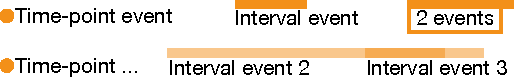
\includegraphics[width=.8\columnwidth]{figure2}\caption{Visual representations of events. Top row, left to right: a complete time-point event, a trimmed time-point event, and a aggregate of 10 events. Bottom row, left to right: an interval event, and two overlapping interval events.}
\label{fig:event-representation}
\end{figure}

\subsection{Set}
\subsubsection{Design Overview}
As discussed in Section\note{ref}, Gestalt's principles of grouping are commonly used to show set relationships among events, most effectively are \emph{proximity} and \emph{uniform connectedness}. Therefore, we also apply these two principles in our design: events belonging to the same set are located close together, and the background of an entire set is colored to make its events visually connected.

Spatial grouping is achieved through vertical positioning because the horizontal position of each event is already fixed by its temporal information. Sets are stacked vertically, and each set is further divided into a maximum of three \emph{layers}: the top and the bottom layer for events shared with the set above and below respectively (if they exist), and the middle layer for other events in the set. Figure~\ref{fig:layering} shows an example of a layering for three sets.

\begin{figure}[!htb]
\centering
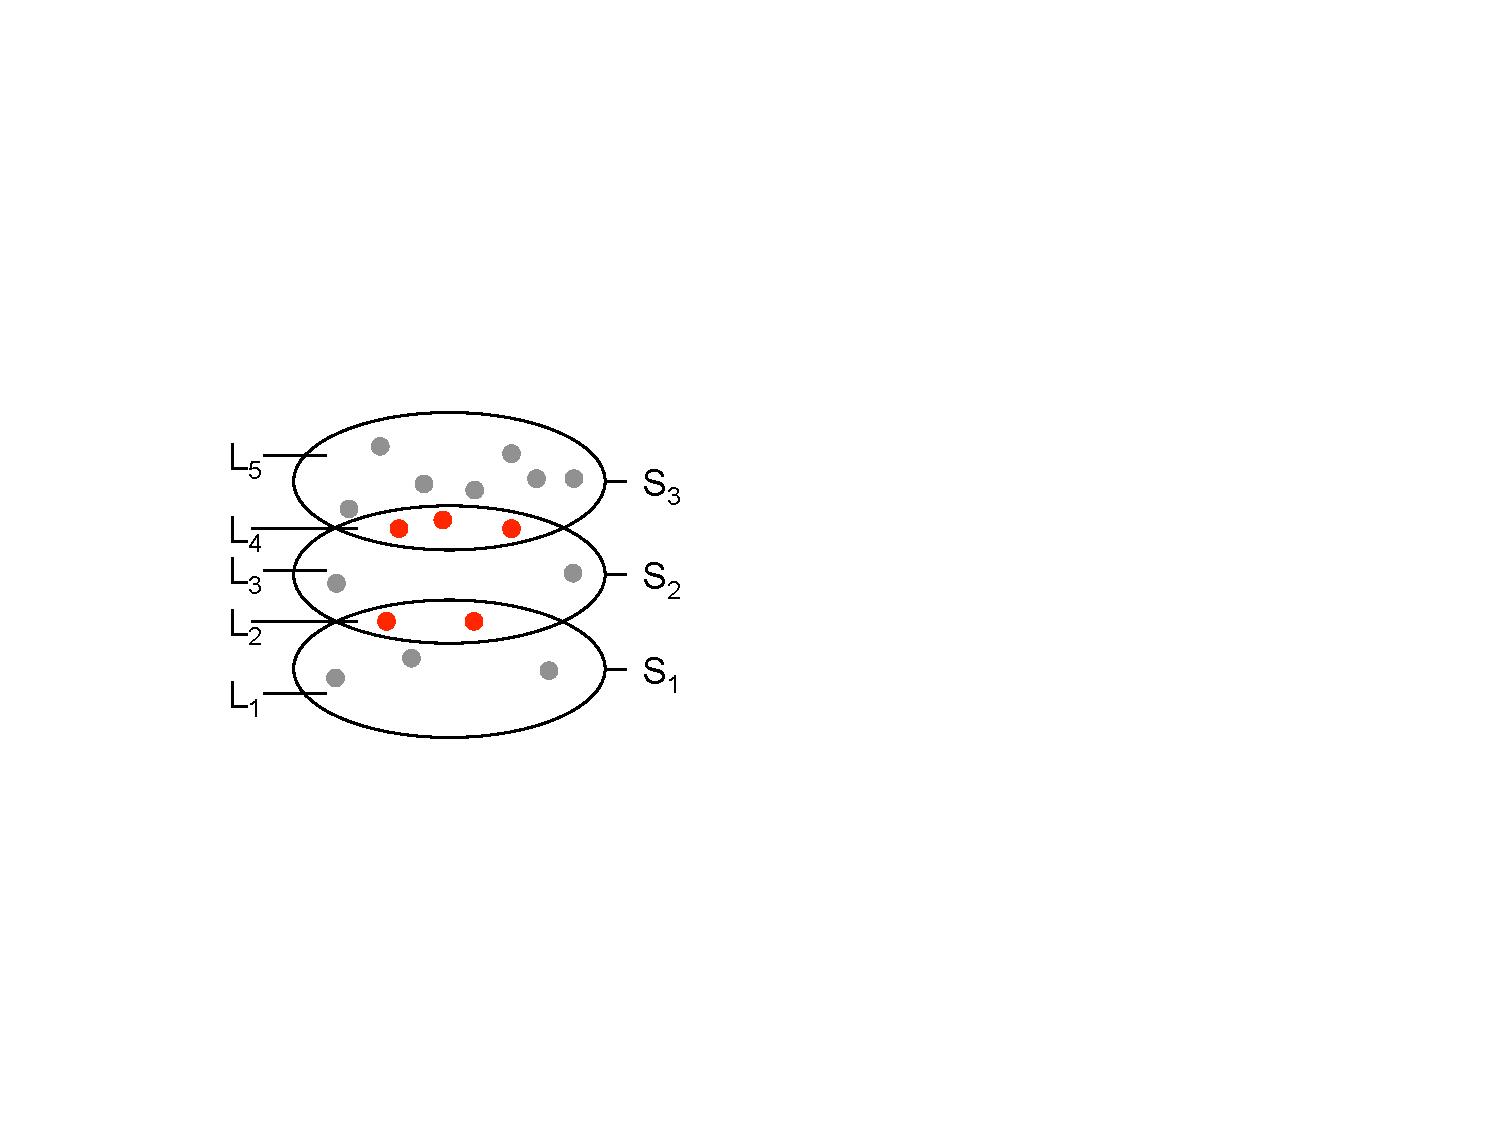
\includegraphics[width=.5\columnwidth]{figure3}
\caption{Layering for three sets $S_1$, $S_2$, and $S_3$. $L_2$ includes events shared by $S_1$ and $S_2$, and $L_4$ includes events shared by $S_2$ and $S_3$. Shared events are shown in red. $S_2$ consists of events in three layers $L_2$, $L_3$, and $L_4$.}
\label{fig:layering}
\end{figure}

Shared events between two non-neighboring sets can reside in one set and connect to the other set using visual links such as curves~\cite{Alper2011} or areas~\cite{Meulemans2013}. Figure~\ref{fig:layering-1} shows an approach to connect shared events (red squares) using straight edges and link them to the orange set to indicate that they also belong to that set. An alternative approach is to duplicate shared events in both sets. In Figure~\ref{fig:layering-2}, red squares are duplicated in both the green and orange sets. Duplication consumes more display space and could make viewers confuse when seeing same events multiple times. However, it ensures all events of the same set being located close together, which makes the visualization compact. Also, a study by Henry Riche and Dwyer~\cite{Riche2010} shows that complex set-intersection shapes reduce readability compared to item duplication. Aiming for a clear visualization, which is crucial for interactive set construction, we decide to duplicate events that belong to non-neighboring sets. Confused duplication and scalability will be addressed later using interaction and layout algorithm respectively.

\begin{figure}[!htb]
	\centering
	\subcaptionbox{Shared events are connected by edges in the green set, and linked to the orange set.\label{fig:layering-1}}[.47\columnwidth]
	{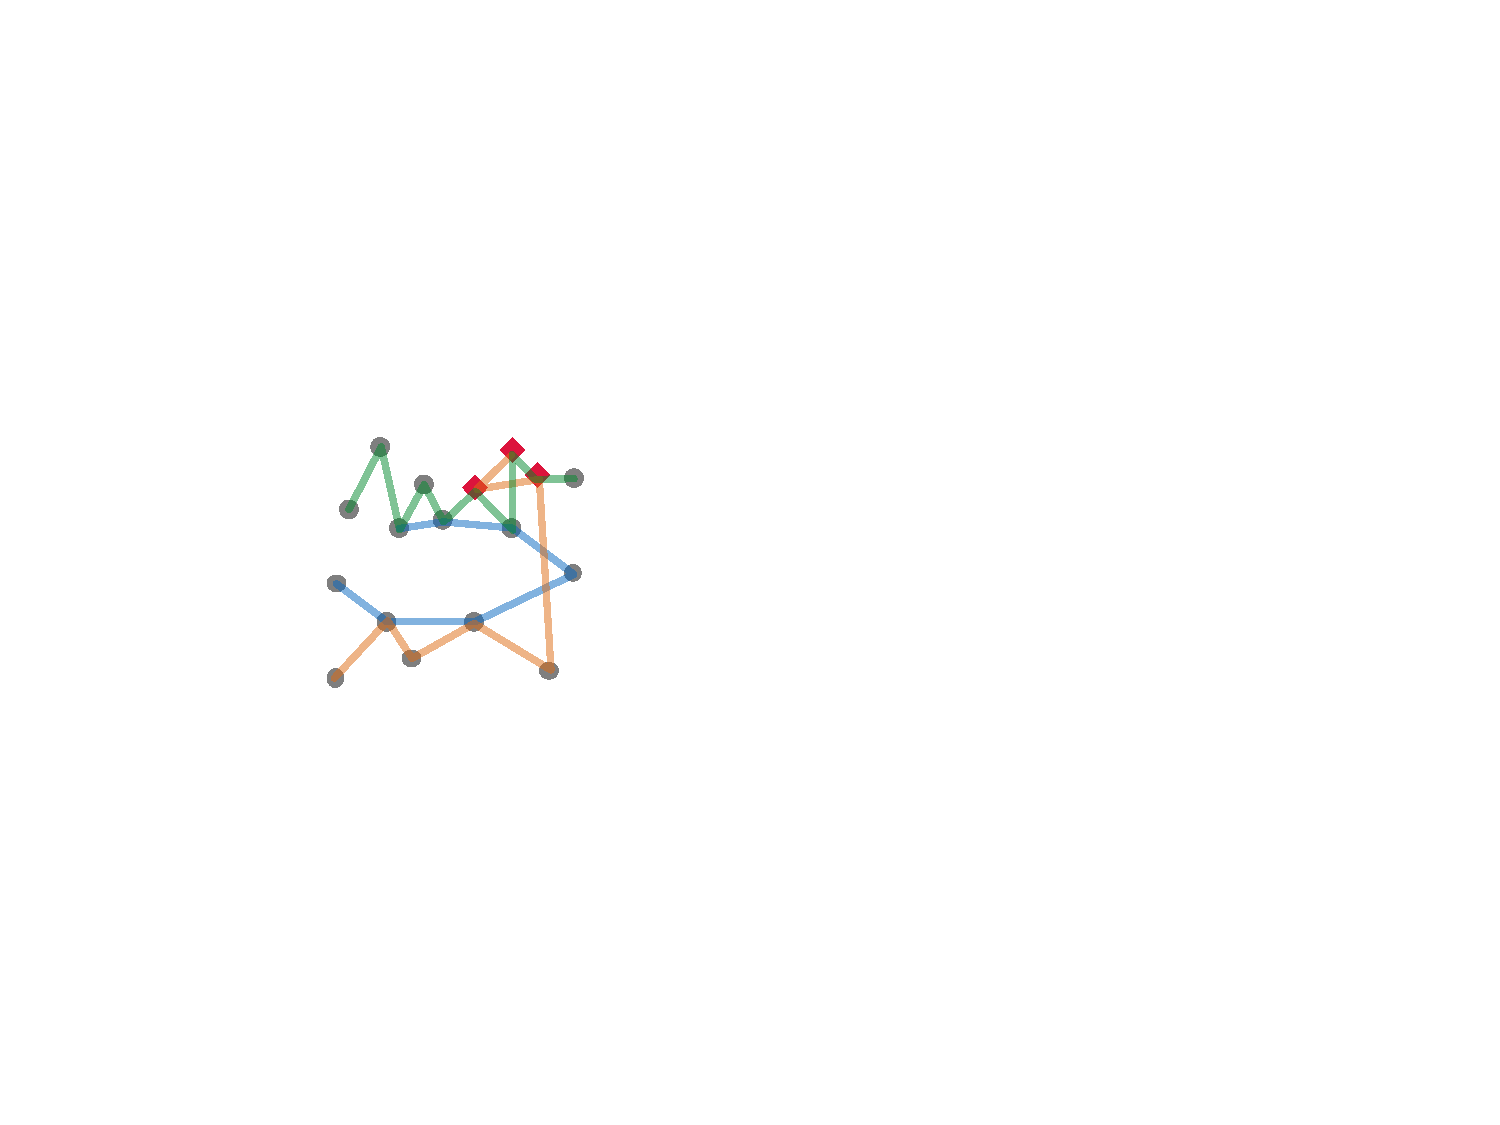
\includegraphics[width=.35\columnwidth]{figure4a}}
	\hfill	
	\subcaptionbox{Shared events are duplicated in both green and orange sets.\label{fig:layering-2}}[.47\columnwidth]
	{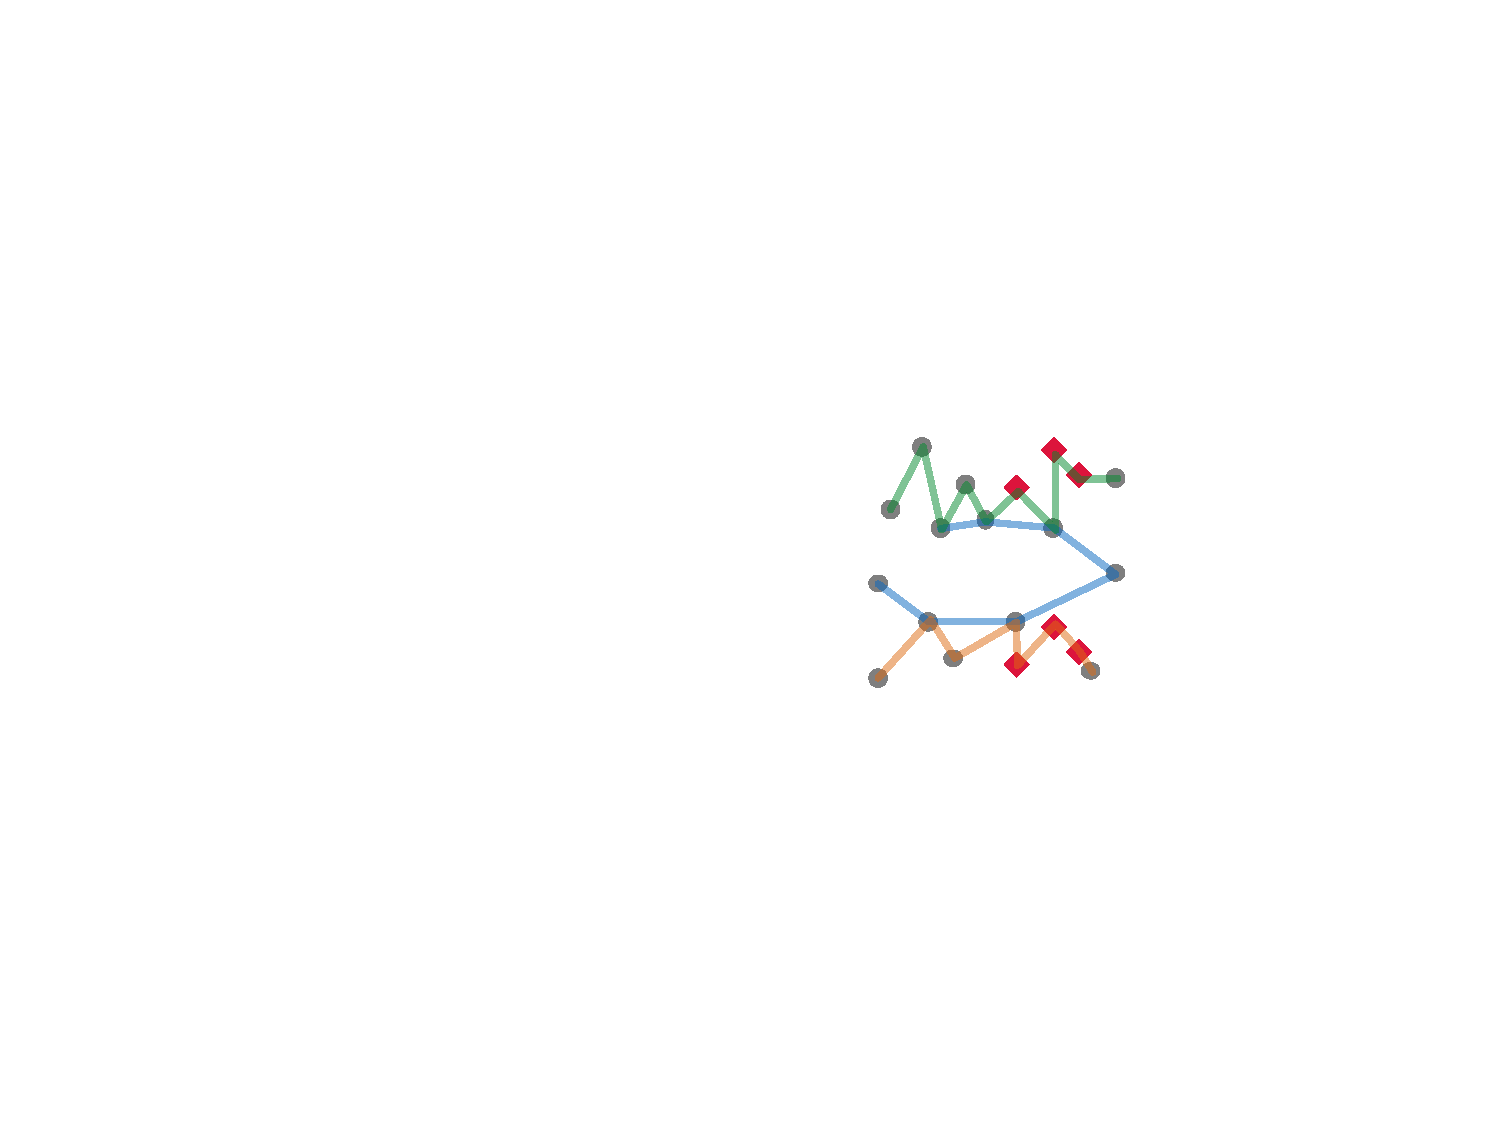
\includegraphics[width=.35\columnwidth]{figure4b}}
	\caption{Shared events (red squares) visualization of two non-neighboring sets.}
	\label{fig:layering-compare}
\end{figure}

In subsequent sections, we discuss the detail of the set visualization algorithm, which consists of two main steps: generating set shapes, and then coloring them.

\subsubsection{Shape Generation}
\label{sub:shapesgeneration}
This algorithm takes as input a list of bounding-boxes of the set's events, and generates a closed-curve containing all these boxes. The sizes and positions of the bounding boxes are decided by the layout algorithm described in the next section. A rectilinear shape can be generated using a scan-line algorithm~\cite{Foley1997}, as shown in Figure~\ref{fig:shape1}. The number of bends along the border is often used to assess the aesthetics and legibility of visualizations~\cite{Tanahashi2012}. Even though the generated shape provides the minimal \textit{data-ink} ratio~\cite{Tufte1986}, a large number of line bends may reduce its legibility. 

\begin{figure}[!htb]
	\centering
	\subcaptionbox{The original rectilinear shape generated by a scan-line algorithm.\label{fig:shape1}} 
	{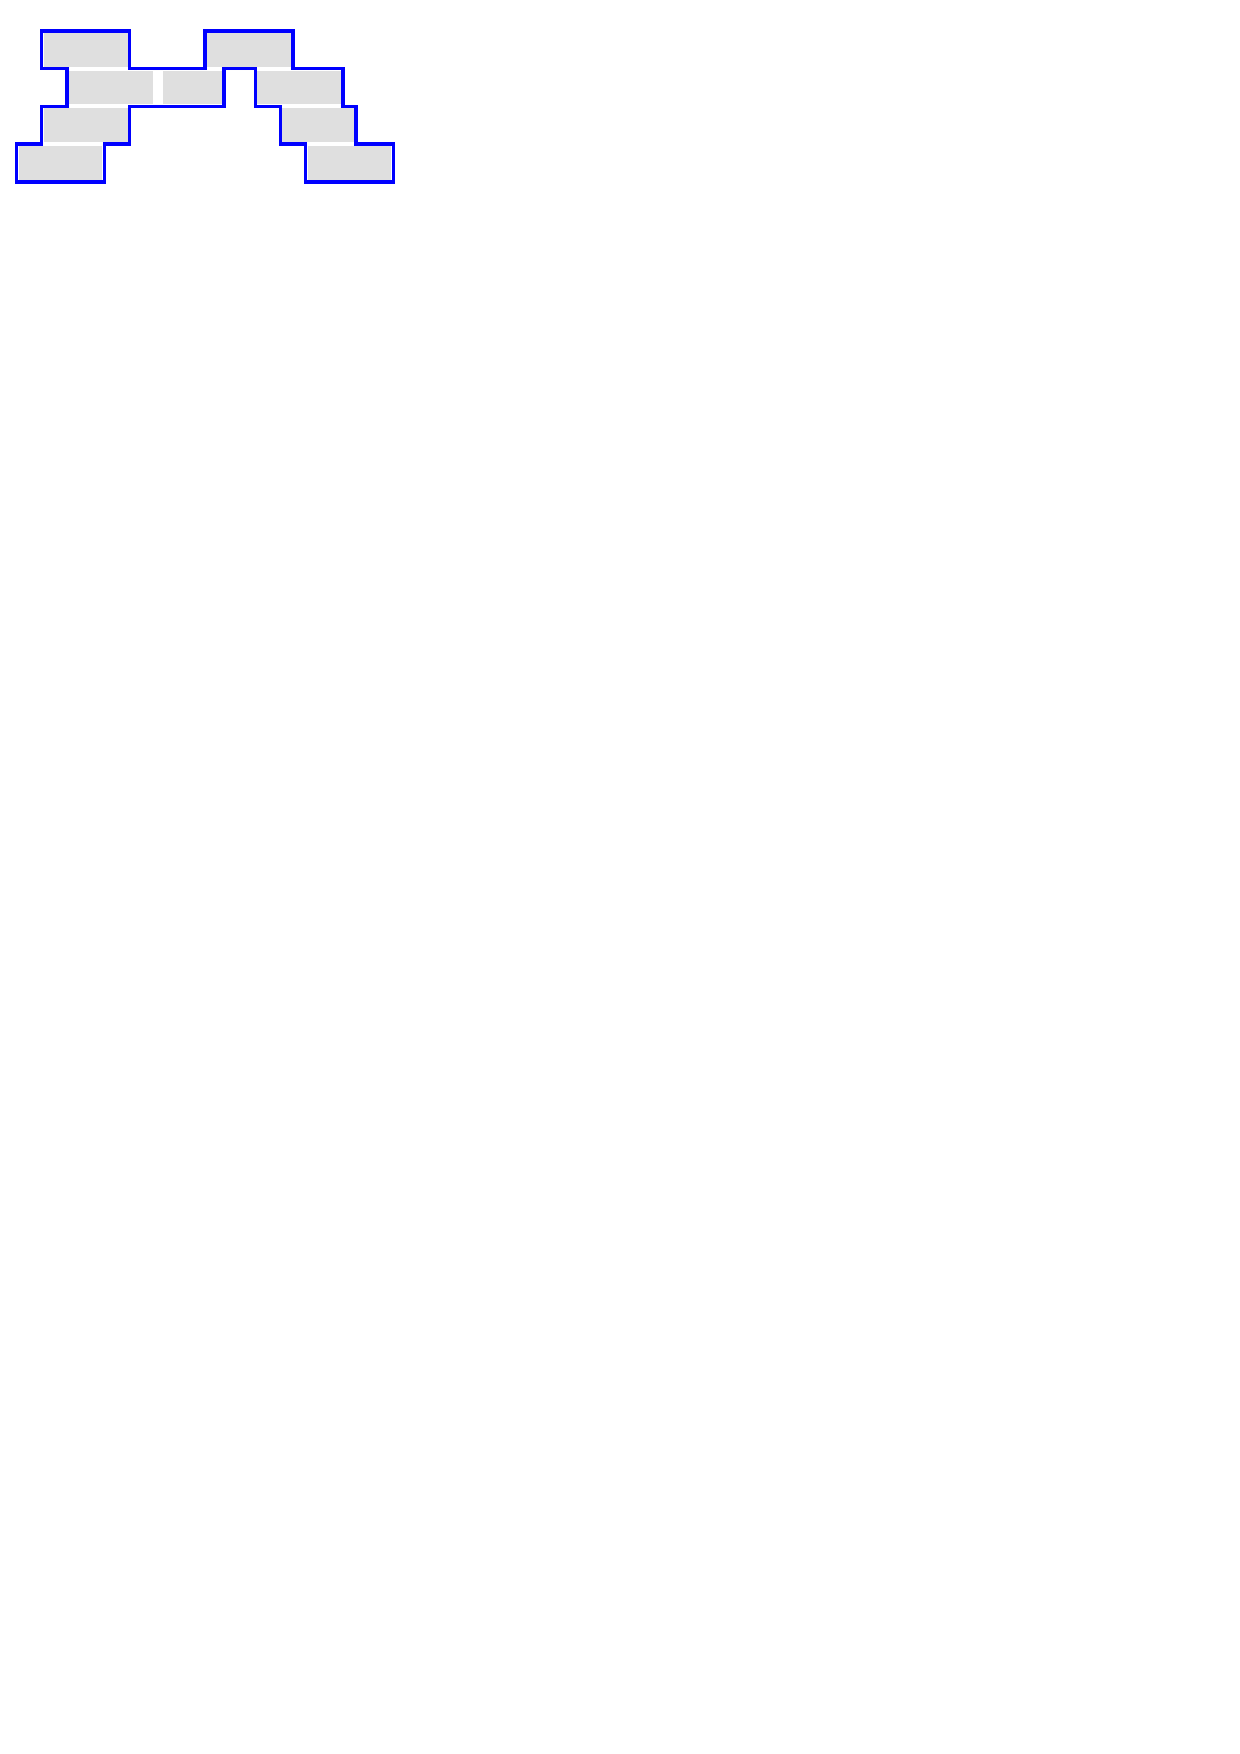
\includegraphics[width=.47\columnwidth]{figure5a}}
	\hfill
	\subcaptionbox{The simplified shape by flattening and removing jags (red eclipse).\label{fig:shape2}}
	{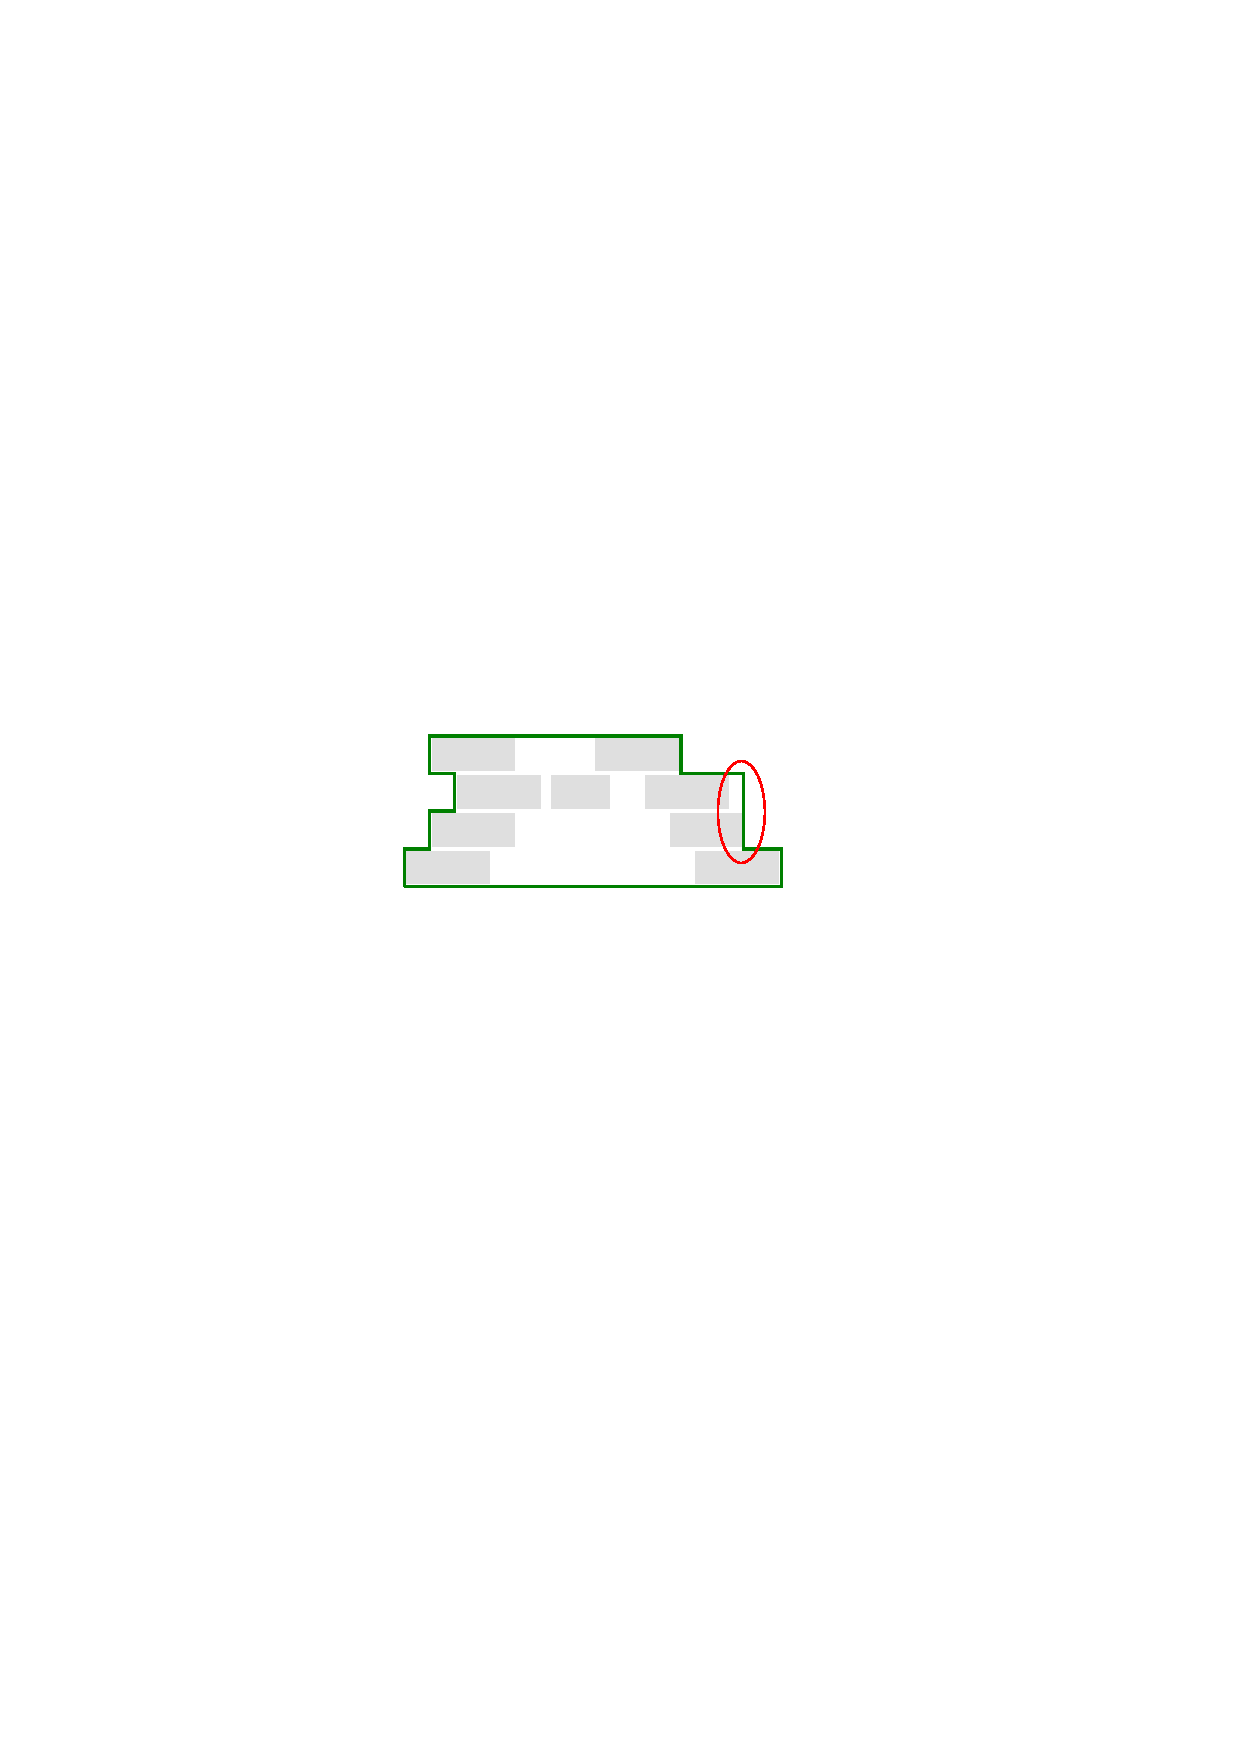
\includegraphics[width=.47\columnwidth]{figure5b}}
	\caption{Rectilinear shape generation.}
	\label{fig:shape}
\end{figure}

To reduce the number of line bends, the top and the bottom sides of the set outline are flattened. The left and right sides  are kept unchanged because they indicate the temporal information of events. On both sides, the outline can be ``jagged'' if two events start or end close to each other. Those close vertical segments are combined to reduce line bends if their horizontal gap is smaller than some threshold. This trades off time accuracy for outline smoothness and can be adjusted by the user. Figure~\ref{fig:shape2} shows the result of this simplification. 

To reduce the degree of line bends, vertical segments are converted to diagonal ones wherever possible, such as  $e_2$ and $e_3$ in Figure~\ref{fig:generation1}. Smoother lines are easier for users to follow~\cite{Kim2010}, thus diagonal segments are further converted to B\'{e}zier curves, and squared corners are replaced by quadrant arcs as in Figure~\ref{fig:generation2}.

\begin{figure}[ht]
	\centering
	\subcaptionbox{Vertical segments $e_2$ and $e_3$ are converted to diagonal ones (dashed lines).\label{fig:generation1}}
		{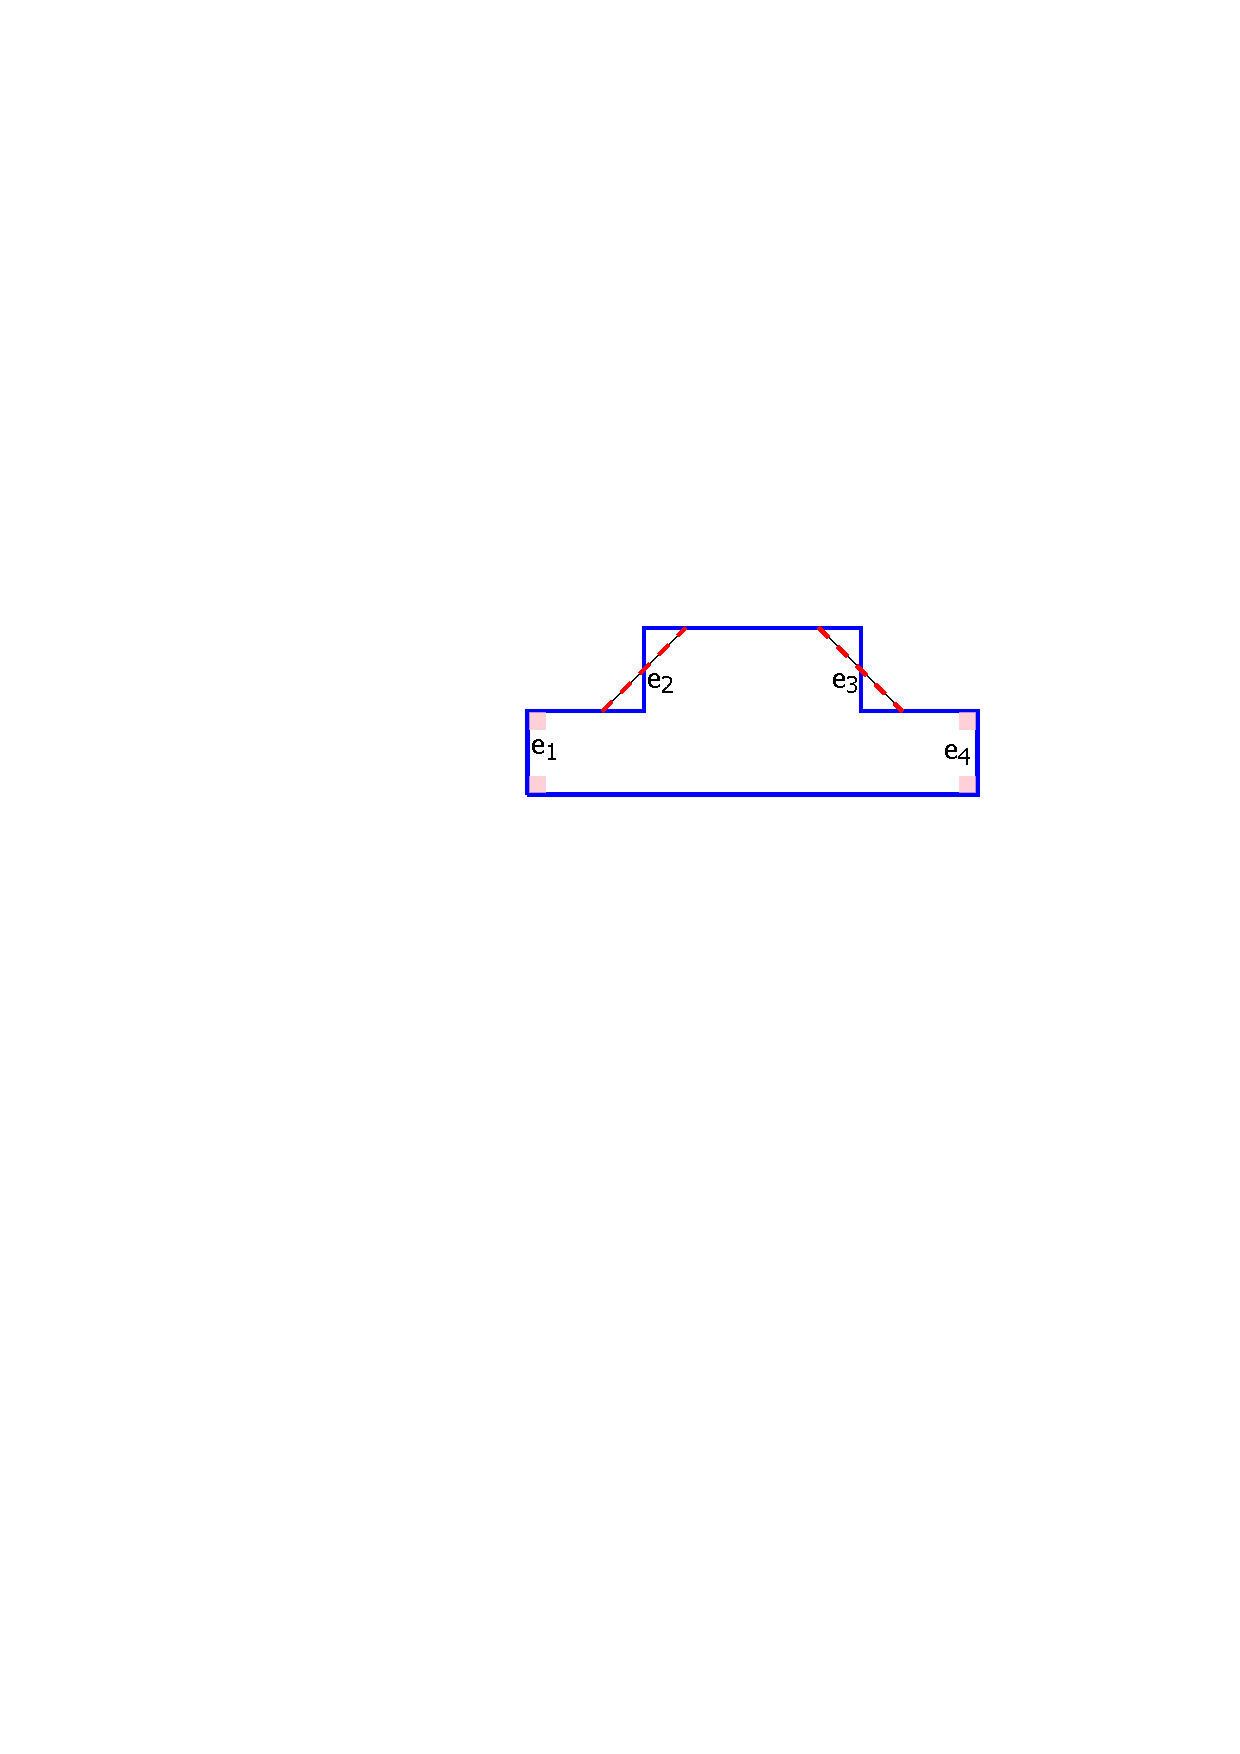
\includegraphics[width=.47\columnwidth]{figure6a}}
	\hfill
	\subcaptionbox{Squared corners are replaced by quadrant arcs. $e_2$ and $e_3$ are smoothened by B\'{e}zier curves.\label{fig:generation2}}
		{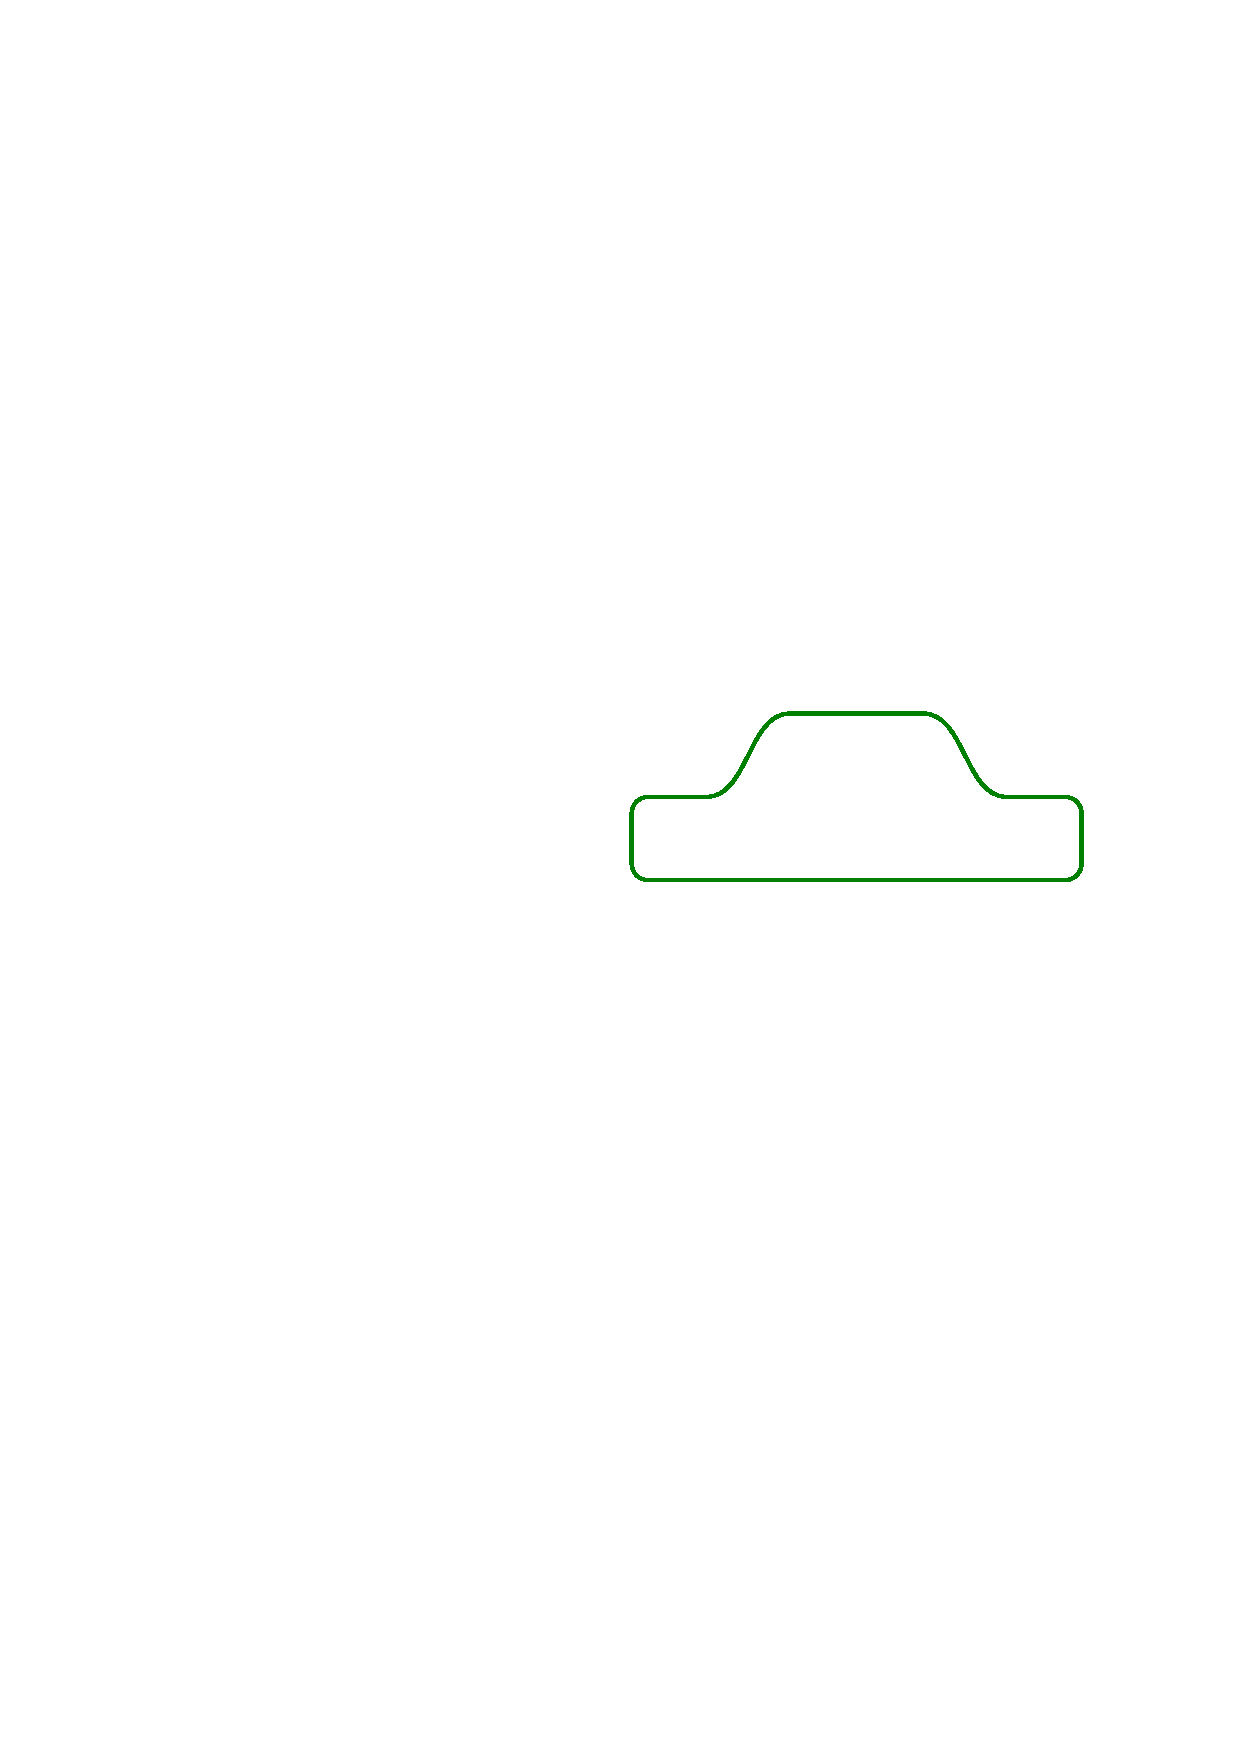
\includegraphics[width=.47\columnwidth]{figure6b}}
	\caption{Shape smoothening by reducing the degree of line bends.}
	\label{fig:generation}
\end{figure}

\subsubsection{Set Coloring}
Each set is filled with a color selected from Qualitative Set 2 of ColorBrewer~\cite{Harrower2003} to make them easily distinguishable. Two color filling options are considered: only the time circle and the entire label. Our design follows uniform connectedness principle requiring visual connection among same-set events. When they are visually connected and only their time circles are filled, intersection between edges and text may reduce the readability of the visualization. Figure~\ref{fig:evaluation2} shows an example of KelpFusion~\cite{Meulemans2013} using this approach. In the second option, filling the entire label may produce a false understanding about the temporal information of events. We choose this option and lessen the effect by coloring the gap between events as in Figure~\ref{fig:evaluation1}. It also helps increase the sense of grouping compared to filling only the time circles.

One common coloring method for set intersections is \emph{color blending} as used in Venn diagrams~\cite{Ware2013}. Color for each set is half-transparent, and alpha blending is applied to produce a new color for the intersection. However, the output color may look irrelevant to the two input colors and may be confused as the color for a new set rather than the intersection part.

To address this issue, we fill the intersection with a linear color gradient changing between the two set colors as in Figure~\ref{fig:gradient1}. While the gradient provides a smooth transition, it becomes difficult to recognize the two ends of the intersection. For example, it is not clear from Figure~\ref{fig:gradient1} that the background of the event ``Rove's 4th grand jury appearance'' (the second row from top to bottom) is pure yellow or it has a mix of green as well. To solve this problem, multiple color transitions are used instead of a single transition. For instance, in Figure~\ref{fig:gradient2}, the color transitions between green and yellow are repeated multiple times so that both colors are clearly shown in every row of the intersection.

\begin{figure}[!htb]
	\centering
	\subcaptionbox{Intersection shown as a single color gradient.\label{fig:gradient1}}
		{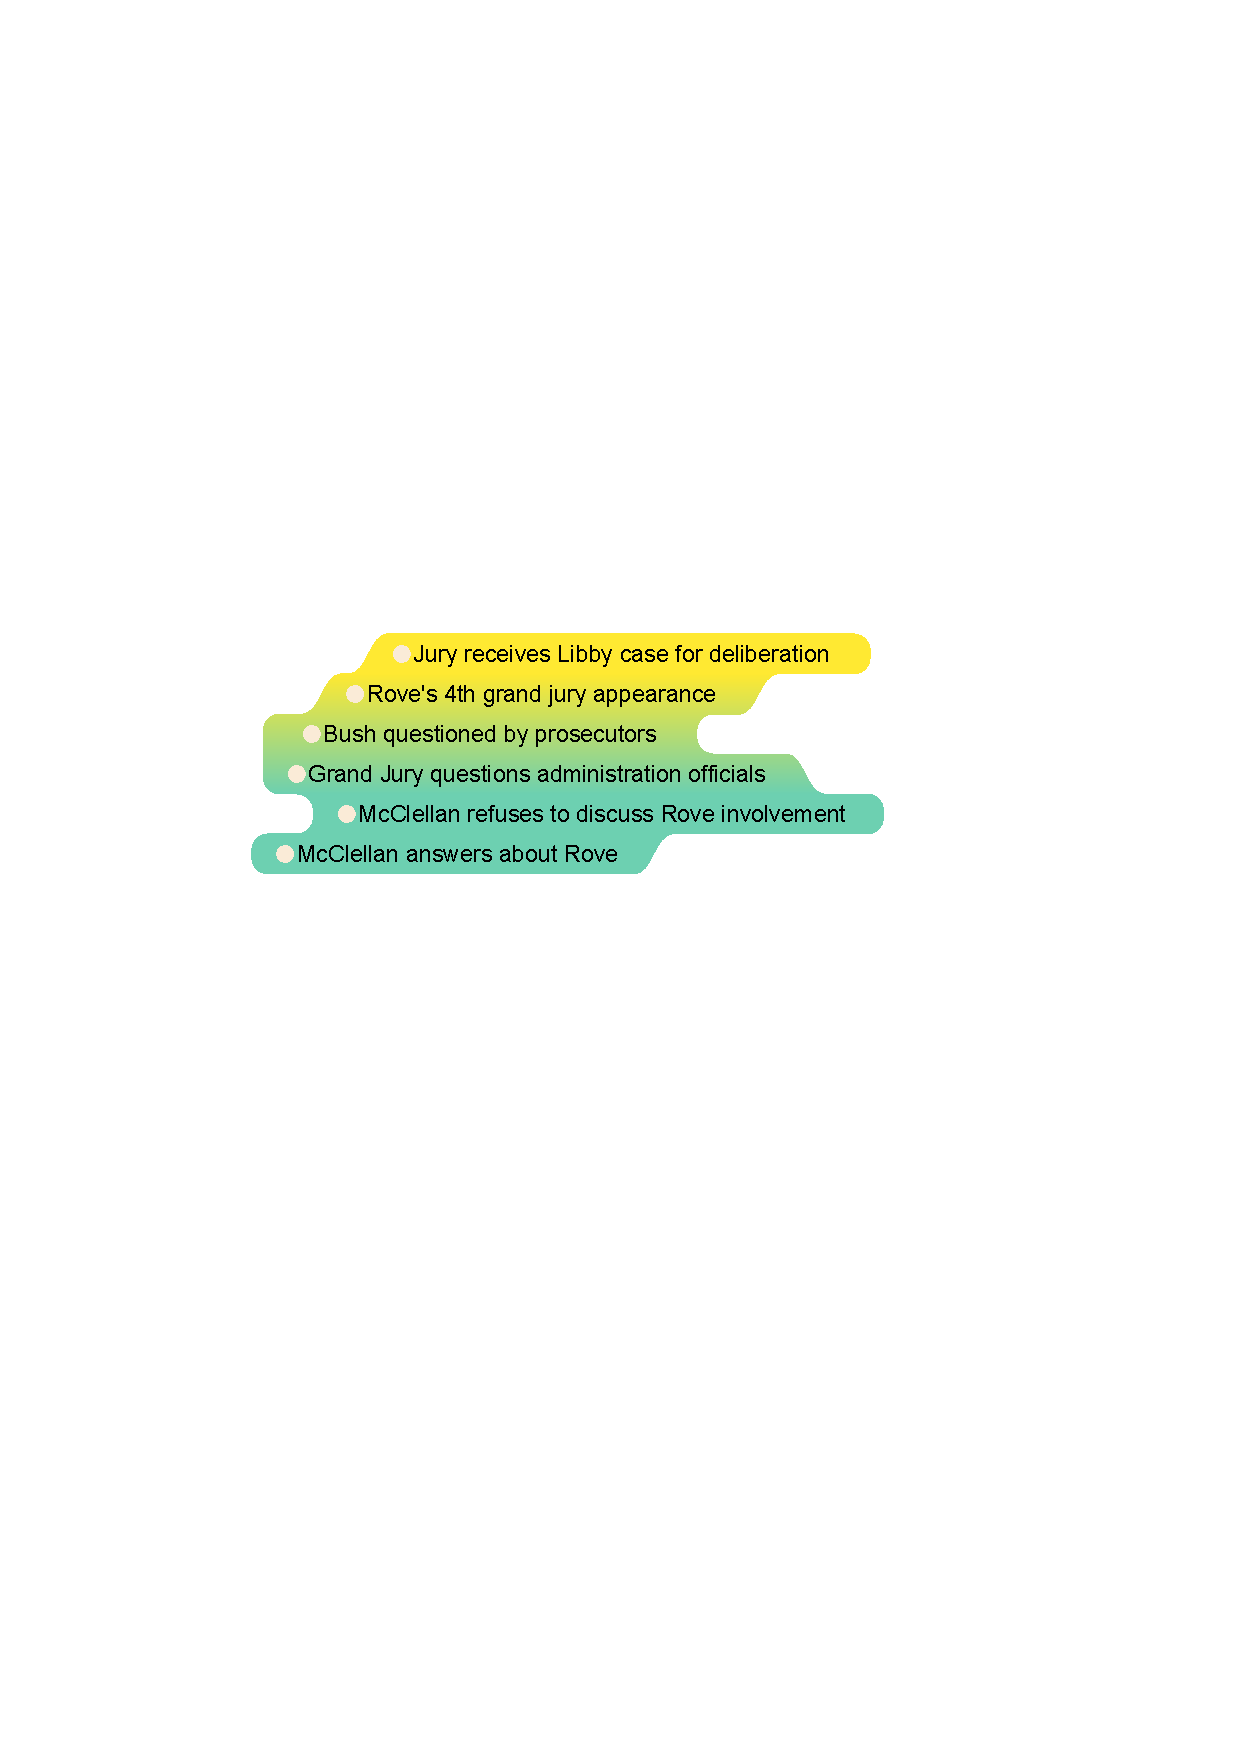
\includegraphics[width=0.47\columnwidth]{figure7a}}
	\hfill
	\subcaptionbox{Intersection shown as multiple color gradients.\label{fig:gradient2}}
		{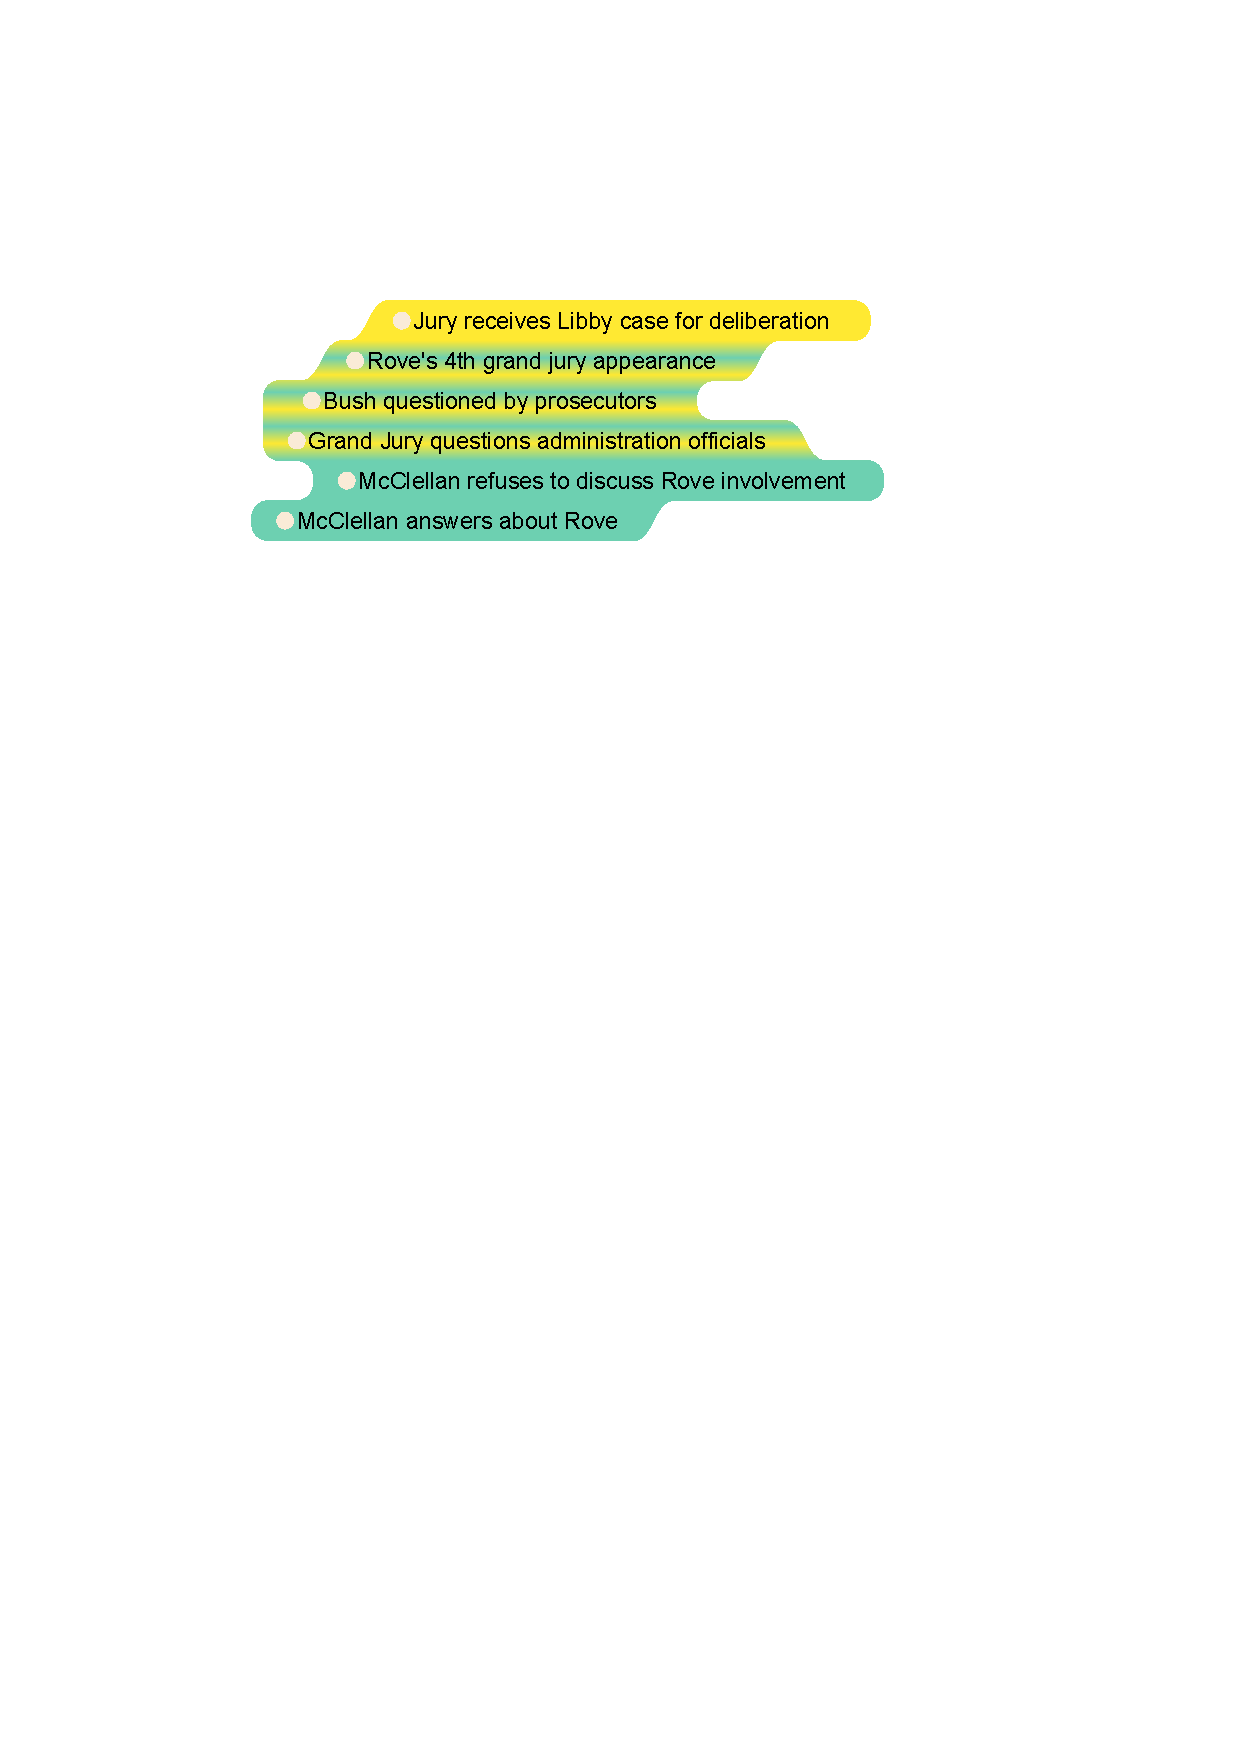
\includegraphics[width=0.47\columnwidth]{figure7b}}
	\caption{Color gradient technique to encode set memberships. The gradient area shows three shared events between two sets.}
	\label{fig:gradient}
\end{figure}

\subsubsection{Multiple-set Events}
With the vertical layering of sets as discussed earlier, three sets cannot be placed adjacently; therefore, it is unable to visualize intersections among three sets or more. This is also a challenging problem with other state-of-the-art methods~\cite{Alsallakh2014}. To address this issue, similar to non-neighboring sets, we replicate events for each set that they belong to so that all events in the same set stay close together producing a compact visualization. To provide full set memberships of events, one method is connecting all replicates of the same event using edges. However, this may produce a cluttered visualization with many edge crossings. Another method is to color code the event according to its set memberships. The first option is to color the event time circle using either multiple circles (Figure~\ref{fig:eventmembership1}) or concentric rings (Figure~\ref{fig:eventmembership2}). The former requires more horizontal space, whereas the latter needs more vertical space. Another option is to color the background of the event label. Color gradient is used for a smooth color transition as in Figure~\ref{fig:eventmembership3}. This visual encoding is consistent with the use of color gradient to show two-set intersections. However, a timeline with many long-label events may produce a too colorful and distracted visualization. Also, limited label height may hamper the detection of color transition. To solve these problems, color is transitioned from left to right, and only run through a first few characters of the event label (Figure~\ref{fig:eventmembership4}). Figure~\ref{fig:citations} shows this technique in a visualization of 200 events.

\begin{figure}[ht]
	\centering
	\subcaptionbox{Each circle represents a set.\label{fig:eventmembership1}}[.22\columnwidth]{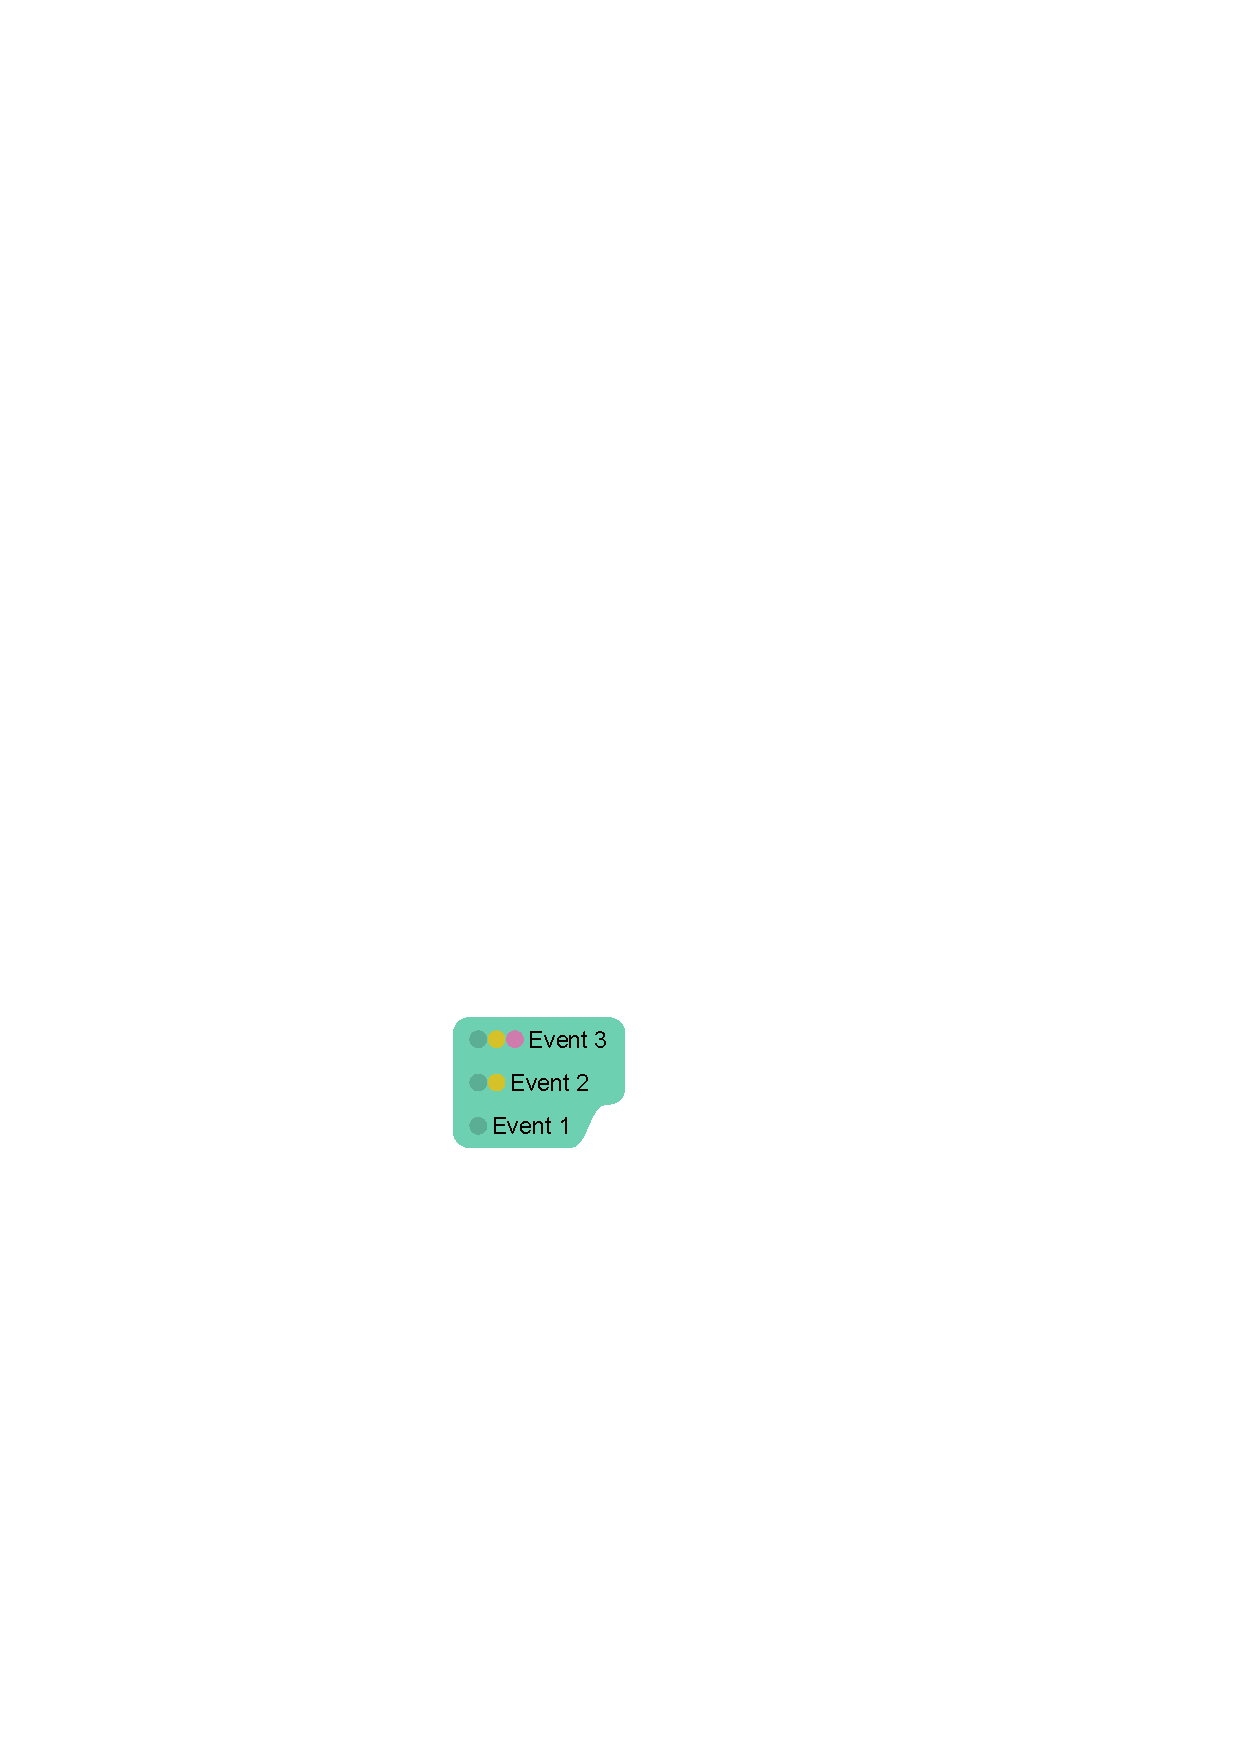
\includegraphics[height=.18\columnwidth]{figure8a}}
	\hfill
	\subcaptionbox{Each ring represents a set.\label{fig:eventmembership2}}[.22\columnwidth]{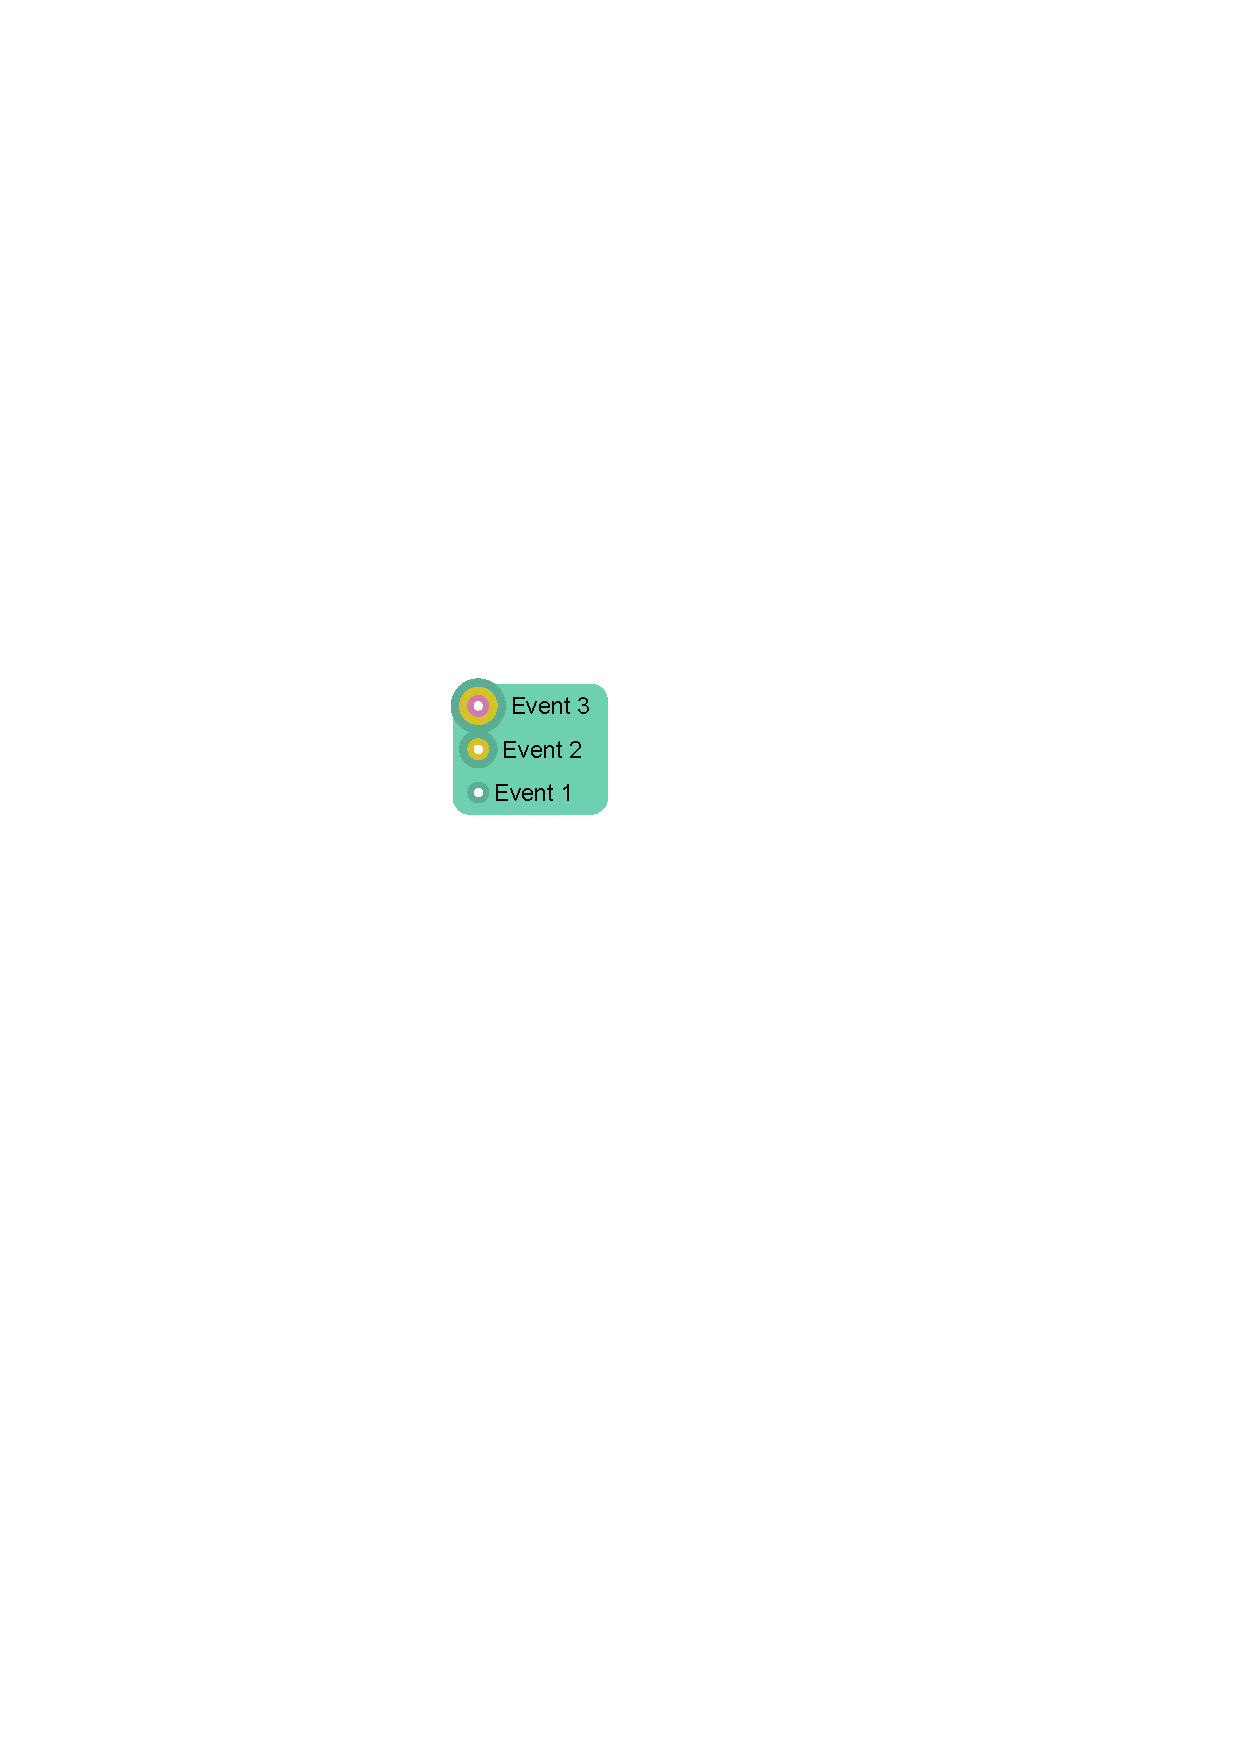
\includegraphics[height=.19\columnwidth]{figure8b}}
	\hfill
	\subcaptionbox{Vertical gradient: each color represents a set.\label{fig:eventmembership3}}[.22\columnwidth]{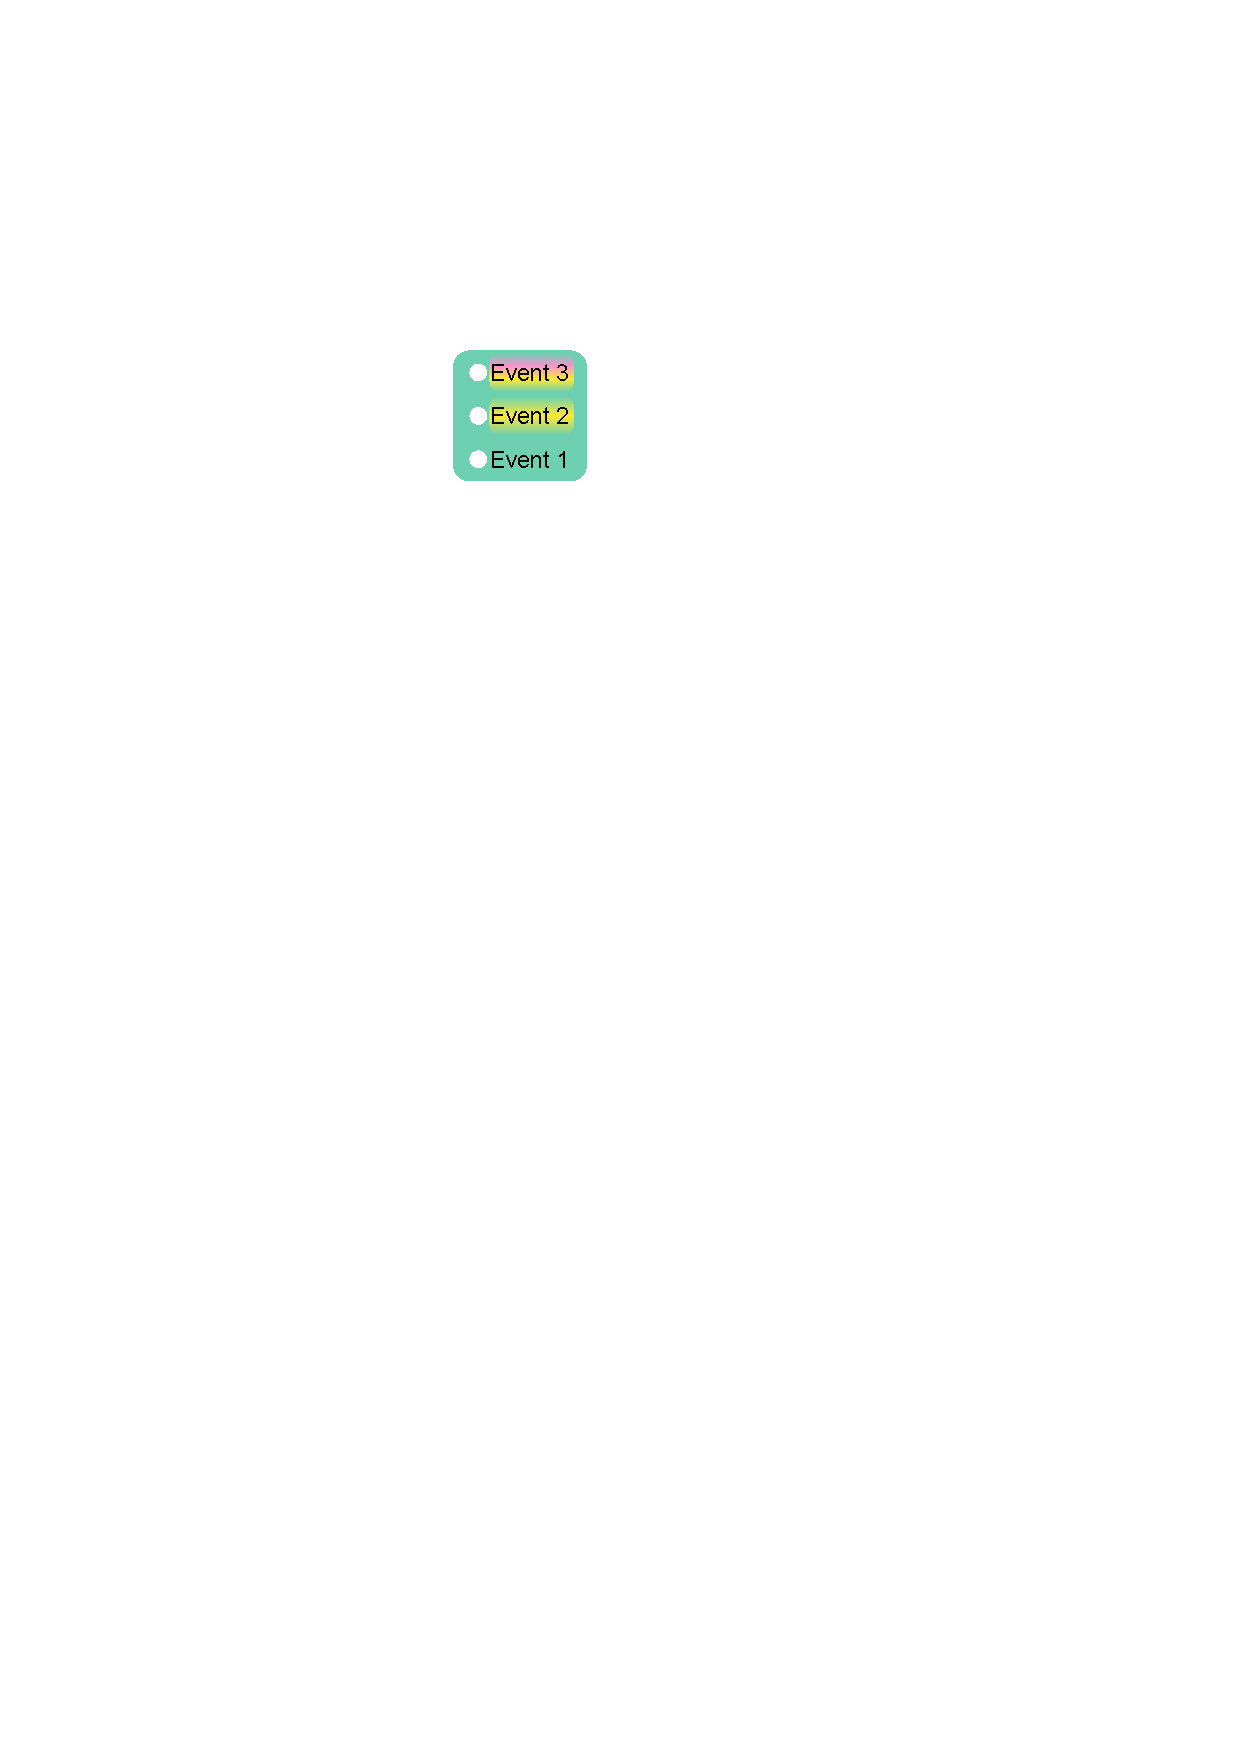
\includegraphics[height=.18\columnwidth]{figure8c}}
	\hfill
	\subcaptionbox{Horizontal gradient: each color represents a set.\label{fig:eventmembership4}}[.22\columnwidth]{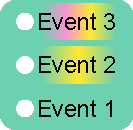
\includegraphics[height=.18\columnwidth]{figure8d}}
	\caption{Multiple-set events visual representation. Event 1 is single-set. Event 2 is double-set. Event 3 is triple-set.}
	\label{fig:eventmembership}
\end{figure}

For interval events, only coloring the background of labels can be used because they do not have time circles, which can be added but at the cost of extra display space. Time bars can be used to show set memberships by dividing into multiple horizontal parts, each color for one set. However, this could be misinterpreted as an event having different set membership in each part of its timespan.



\label{sub:interaction}
Interactive features are implemented to support timeline exploration. Mouse hovering an event reveals its temporal information and the complete label. When none of the multiple-set visualization techniques proposed earlier is used to statically display the full set memberships of an event, it is possible to use interaction to reveal that information. When an event is hovered, all of its replicates are highlighted enabling easy examination of the its full set memberships. This method prevents adding extra ink to the visualization; however, it requires users to discover the set information manually. 

TimeSets provides interactive set filtering and focused time window changing via zooming and panning. Clicking on a set in the legend (bottom-right corner in Figure~\ref{fig:teaser}) toggles its visibility. Time zoom is performed via the mouse-wheel button and pan is controlled by dragging the left mouse button. Users can also interactively modify set ordering by changing the order in the legend through drag-and-drop. A smooth animated transition is provided for all the interactions to help users maintain their mental maps~\cite{Elmqvist2011}.
\section{Layout}
\label{sec:ts-algorithm}
The layout algorithm to produce the positions of sets and events within them consists of four steps. First, the vertical ordering of sets is computed to ensure that two sets that share events are next to each other wherever possible. Then, sets are further divided into layers, and events are assigned to these layers according to their memberships. After that, the position and length of each event are computed, within the given display space. Finally, layers are compacted to remove any gaps between them, before their sizes are adjusted to yield a consistent level of detail across all sets.

\subsection{Sets Ordering}
\label{sec:set-ordering}
This step aims to maximize the number of events shared by neighboring sets, and can map to a graph path problem. Given a list of sets $S=\{s_1, s_2, \dotsc, s_n\}$, an undirected graph $G = (V,E)$ is created with each vertex $v_i$ representing a set $s_i \in S$. Two vertices $v_i$ and $v_j$ are connected if $s_i$ and $s_j$ share an event. The weight of edge $e_{ij}$ is the number of events shared by $s_i$ and $s_j$. Finding a set order with the maximum number of events shared by neighboring sets is equivalent to finding a path with the maximum weight connecting all vertices in $G$. This longest path problem is known to be NP-hard. However, the number of sets we plan to support is constrained by the number of colors that human can easily distinguish when they are shown together, which are only around 12 colors~\cite{Munzner2014}. Therefore, we decide to use a brute-force approach to find the optimal solution.

\subsection{Layer Layout}
% Requirements
This step positions all the events within a layer. Its input includes:
\begin{itemize}
	\item The events belonging to the layer with their \emph{label} and \emph{time} values.
	\item The maximum width and height of the layer.
\end{itemize}

The output includes locations of the input events within the constrained display area, optimized for the following criteria:
\begin{description}
	\item[Completeness] measuring how much event labels are visible. More specifically, we define the \emph{completeness ratio} as:
	$\theta = \frac{\alpha \cdot |E_c| + \beta \cdot |E_t|}{|E|}$, where $|E_c|$ is the number of complete events, $|E_t|$ is the number of trimmed events, and $|E|$ is the number of all events. $\alpha$ and $\beta$ are the coefficients to indicate how strongly complete events and trimmed events contribute to the overall content richness of the layer, respectively. We practically set $\alpha=1$ and $\beta=0.5$.

	\item[Traceability] measuring how easy to follow the events within a layer chronologically. Events happened close in time should have small changes in their row levels to maintain the reading flow. More specifically, we define the \emph{traceability ratio} as:
	$\gamma=\frac{\sum\limits_{i=1}^{|E|}(|l_{i+1} - l_i|)}{|E|-1}$	, where $|E|$ is the number of all events within the layer and $l_i$ is the row level of event $e_i$.
\end{description}

The horizontal position of an event is fixed by its time. The layout therefore decides on which row to position an event; i.e., vertical position, and the level of detail for its label.

\subsubsection{Completeness Layout}
This layout aims to display events with as much content as possible. Starting with an empty layer, events are processed chronologically. An event is located at the possibly lowest row where it does not overlap with any other events. If such a row does not exist (because it reaches the height limit of the display), one of the earlier located events is trimmed to make space for that event. Among these events, the one with the least text being trimmed is selected. However, if the label space of that event is too short for a single word after trim, it will combine with the current event to form a new aggregated event labeled ``2 events''. Aggregated events cannot be trimmed, thus if a new event overlaps with them, it will be added into the existing aggregate. For example, a new event that overlaps with a ``2 events'' aggregated event will be grouped together producing the ``3 events'' aggregate.

The completeness layout maximizes the number of complete events $|E_c|$ and trimmed events $|E_t|$, thus yielding a maximum completeness ratio $\theta$. However, this layout does not optimize traceability because an event is located in the possibly lowest row disregarding the row level of its preceding event.

\subsubsection{Traceability Layout}
To improve traceability, this layout inserts a new event at the same row as its preceding event. If they overlap, the preceding event is trimmed to make space for the currently adding one. We define the \emph{trim ratio} of an event as the ratio of the remaining text length to its original length. An event can only be trimmed if the resulting trim ratio is greater than a minimum threshold $t_{min}$, where $0\leq t_{min} \leq 1$. This value determines how much completeness can be traded for traceability. If the resulting trim ratio is smaller than $t_{min}$, the event moves up or down, up to $r_{max}$ rows on both sides, to find a satisfied row. $r_{max}$ decides how far, in terms of row level difference, an event can be from the preceding event, which essentially trades traceability for completeness. If no suitable row can be found within $\pm r_{max}$ rows, the currently adding event returns to the level of its preceding event and is then trimmed or aggregated with the preceding event as in the completeness layout.

\autoref{fig:traceability} shows an example of these two layouts. Both  run with linear time in terms of the number of events, because during the event insertion, the completeness layout checks up to a constant number -- the layer height -- of times, and the traceability layout checks at most ($2 \times r_{max}+1$) rows.

\begin{figure}[!htb]
\centering
	\subcaptionbox{Completeness algorithm: $\theta=1$, \\$\gamma=5/3$.}{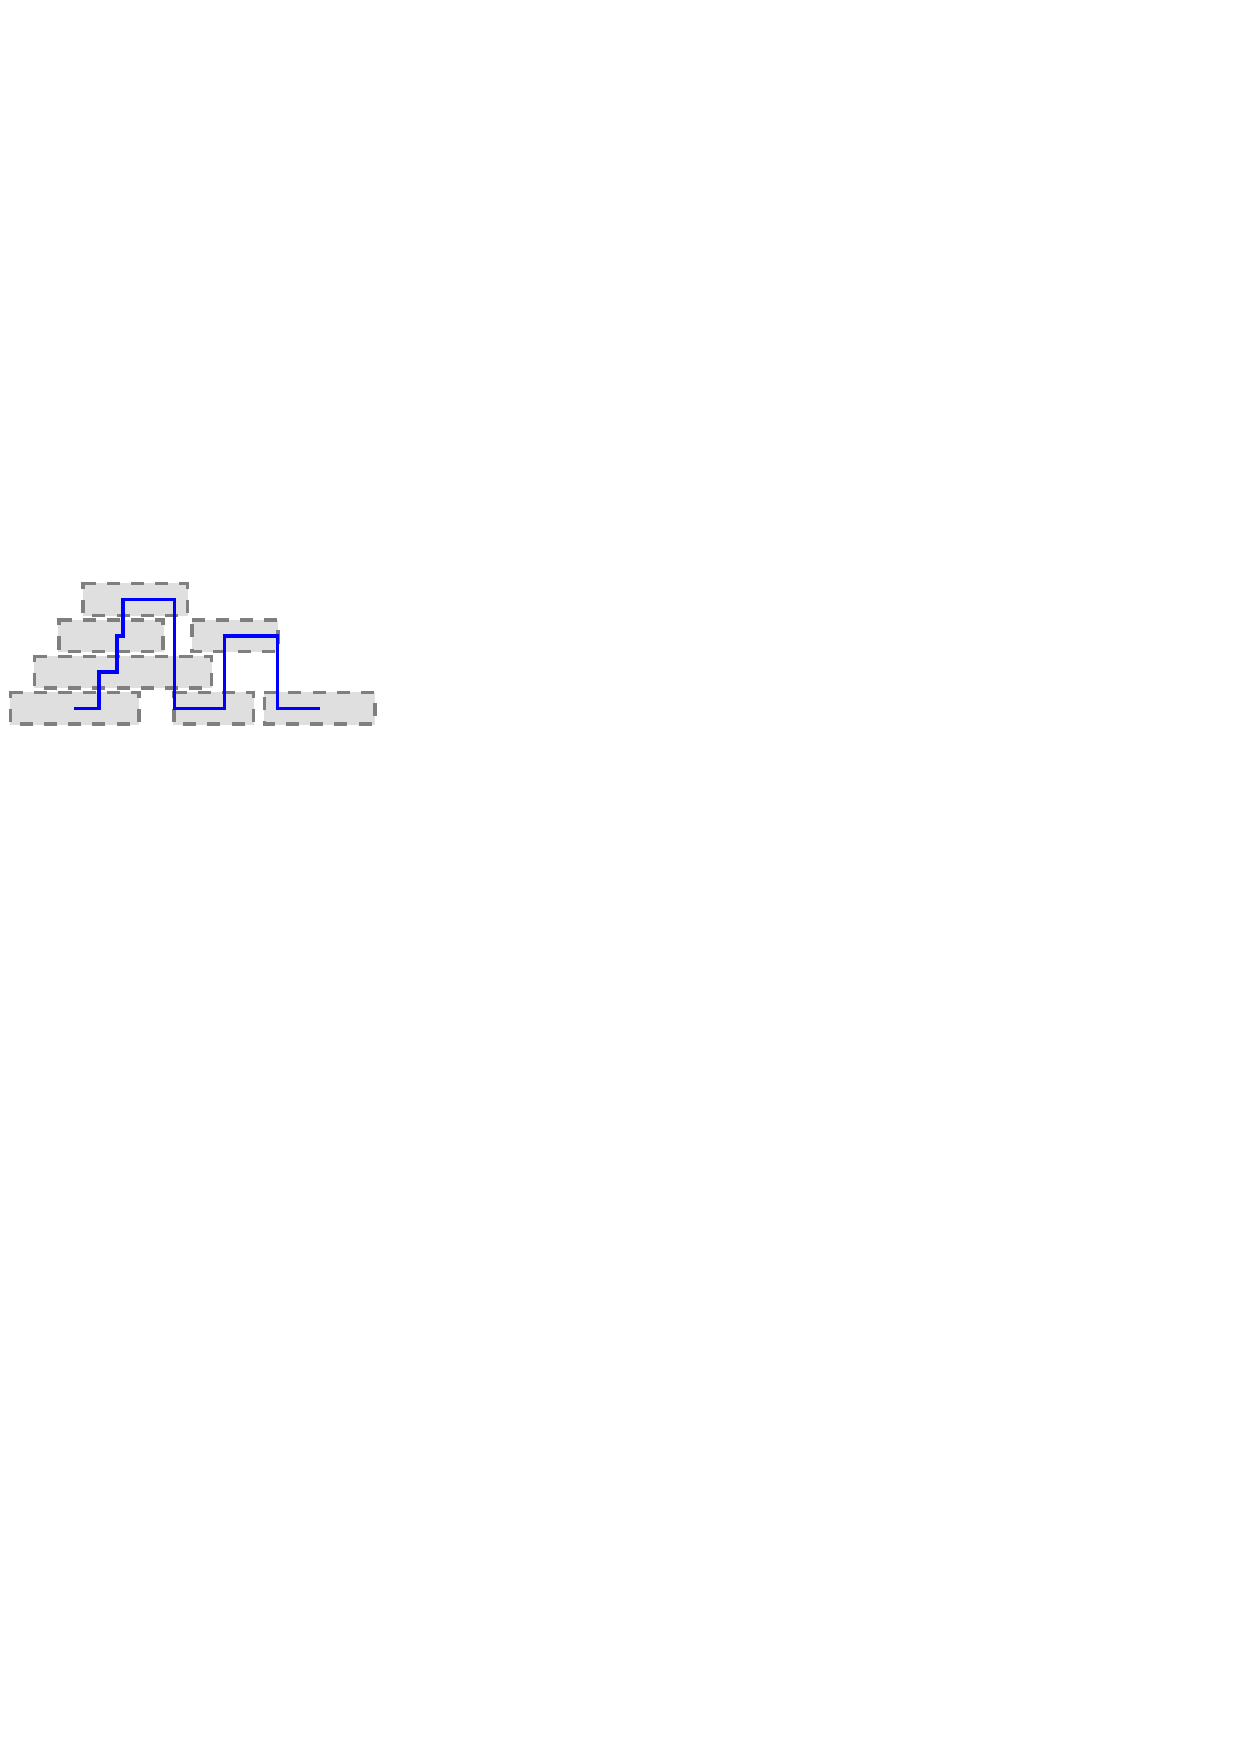
\includegraphics[width=.48\linewidth]{figure9a}}
	\hfill
	\subcaptionbox{Traceability algorithm with $t_{min}=0.5$ and  $r_{max}=1$: $\theta=6/7$, $\gamma=2/3$.}{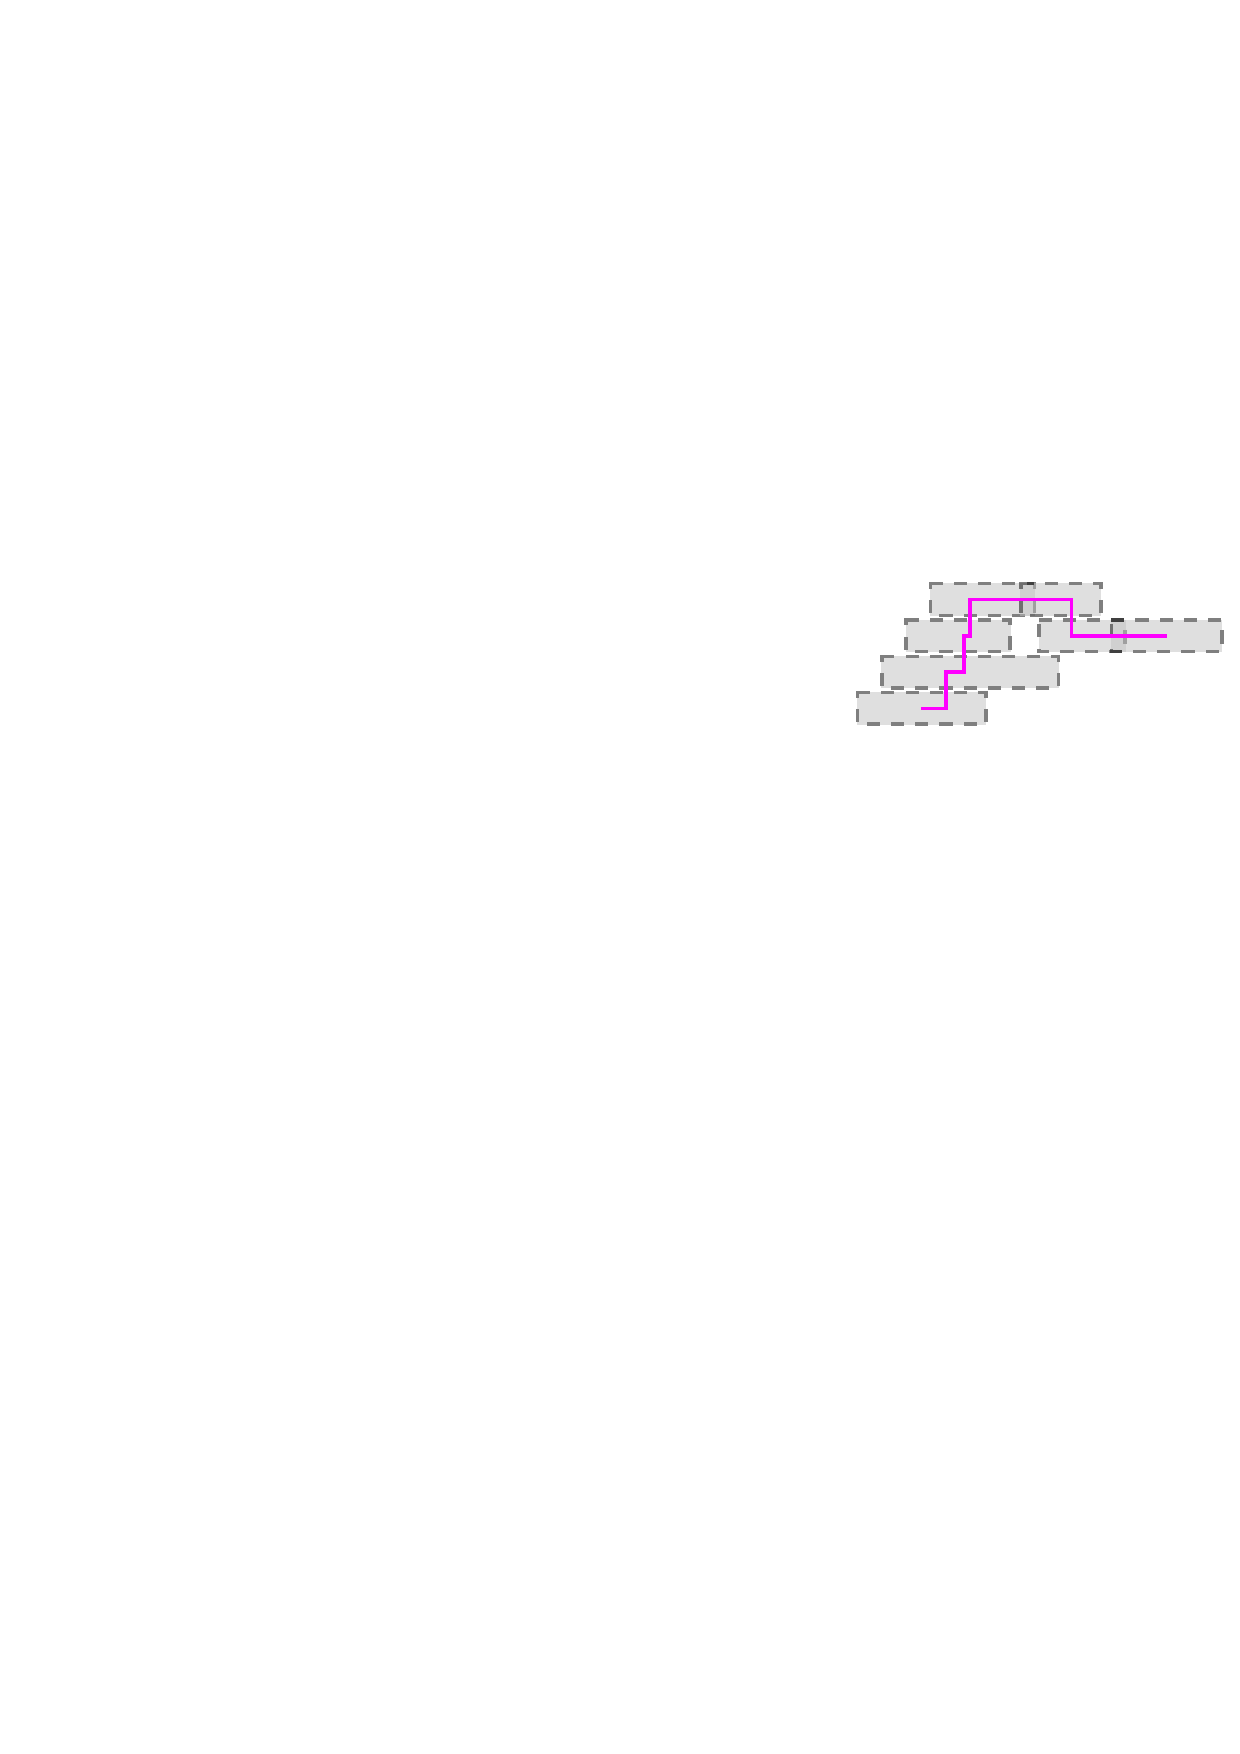
\includegraphics[width=.48\linewidth]{figure9b}}
\caption[Layer layouts]{Layer layouts. Each rectangle represents an event. The line connecting centers of rectangles illustrates the  traceability.}
\label{fig:traceability}
\end{figure}

\subsection{Layers Compacting}
\label{sub:compact}
After the layout of each layer is independently computed, layers are stacked together to produce a compact visualization. The two layer layouts require the layer height input as a maximum number of rows. Initially, that height is assigned proportionally to the number of events within each layer. However, some layers may not use all of their allocated space, resulting gaps between layers that need to be filled. This includes moving two layers closer if there is a gap in between, or moving a layer into a newly created space if its set does not share events with any other sets. The freed space is assigned to the layer with the lowest completeness ratio $\theta$. Then, layouts of all layers are recomputed and compacted again. The process repeats until no more space can be saved. \autoref{fig:compacting} shows an example of compacting.

\begin{figure}[!htb]
	\centering
	\subcaptionbox{Before: consumed height = 6 rows.}{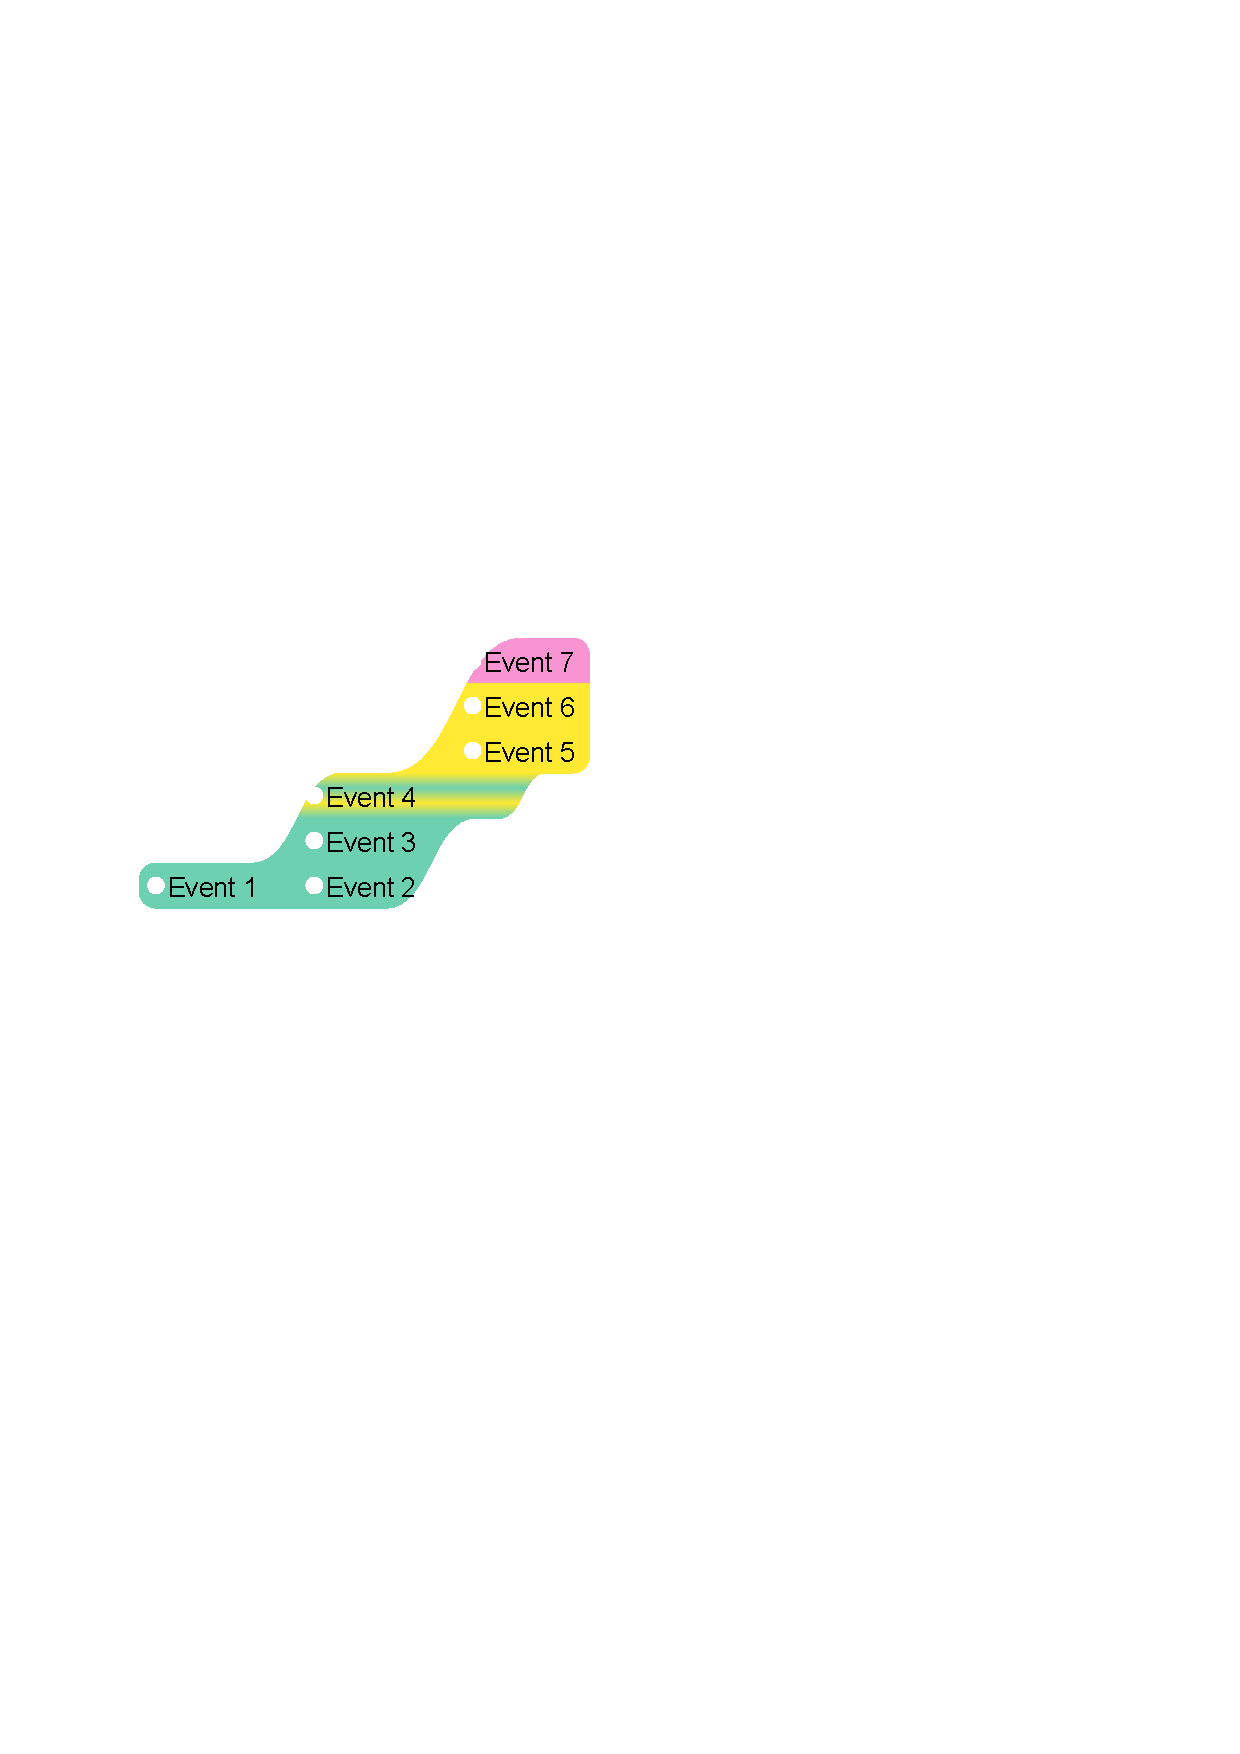
\includegraphics[width=.45\columnwidth]{figure10a}}
	\hfill
	\subcaptionbox{After: consumed height = 3 rows.}{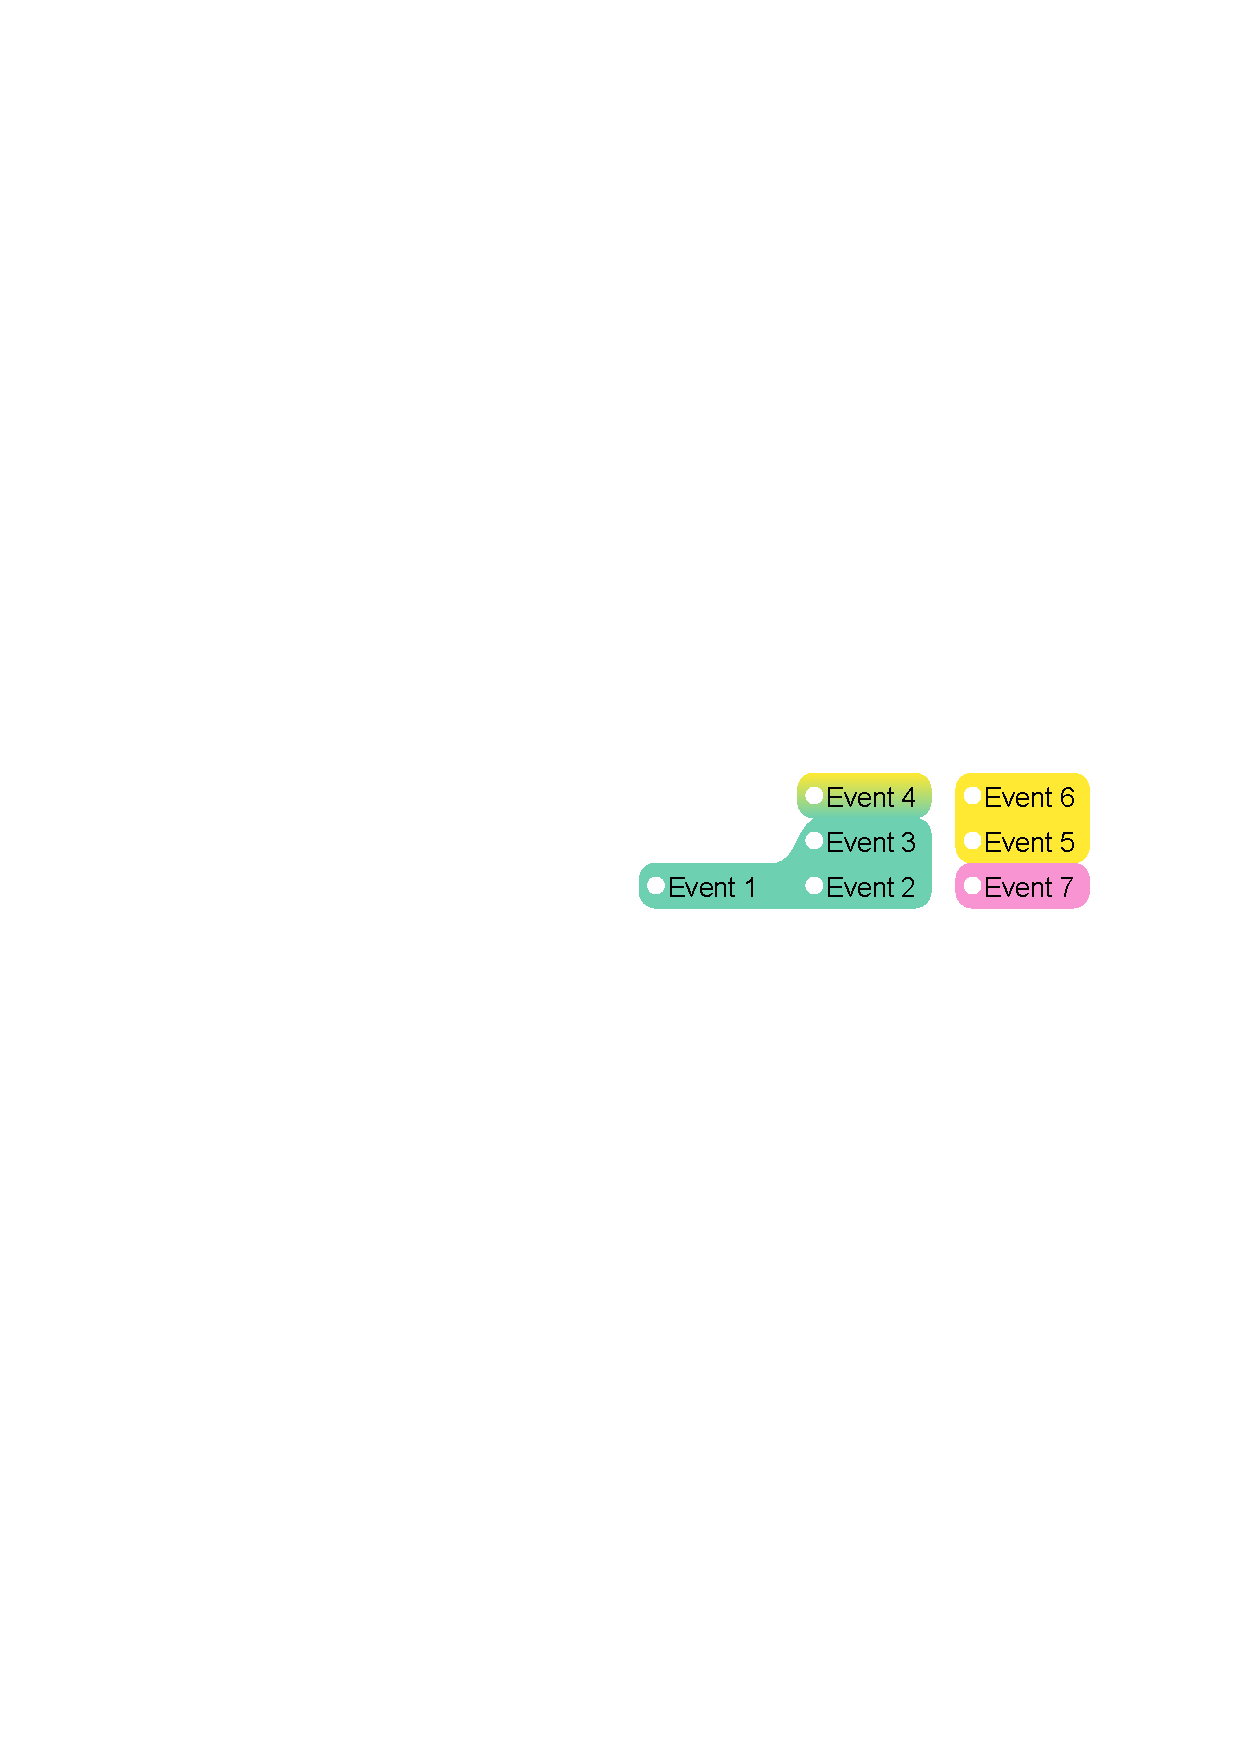
\includegraphics[width=.45\columnwidth]{figure10b}}
	\caption{Layers compacting.}
	\label{fig:compacting}
\end{figure}

\subsection{Layers Balancing}
This last step ensures that all layers have similar levels of detail; i.e., avoiding layers with many complete events and other layers with many aggregated events. This is achieved by minimizing the variance of completeness ratios of all layers,
$\frac{\sum\limits_{i=1}^{n}(\theta_i - \bar{\theta})^2} {n}$, where $n$ is the number of layers and $\bar{\theta}$ is the mean of all completeness ratios. A brute force approach tests all possible combinations of layer height $h_i$ such that $\sum\limits_{i=1}^{n}h_i=H$ for a minimum variance, where $H$ is the height of the display area. However, the number of combinations is an exponential of $n$. Instead, we apply a heuristic that relies on a simple observation that the completeness ratio increases with layer height. Therefore, the algorithm reduces the completeness ratio variance by iteratively transferring a row from the layer with the largest ratio to the layer with the smallest one, until the variance no longer decreases. \autoref{fig:balancing} shows an example of balancing.

\begin{figure}[!htb]
	\centering
	\subcaptionbox{Before: $\theta_{green}=0.25$, $\theta_{yellow}=1$.}{\label{fig:balancing1}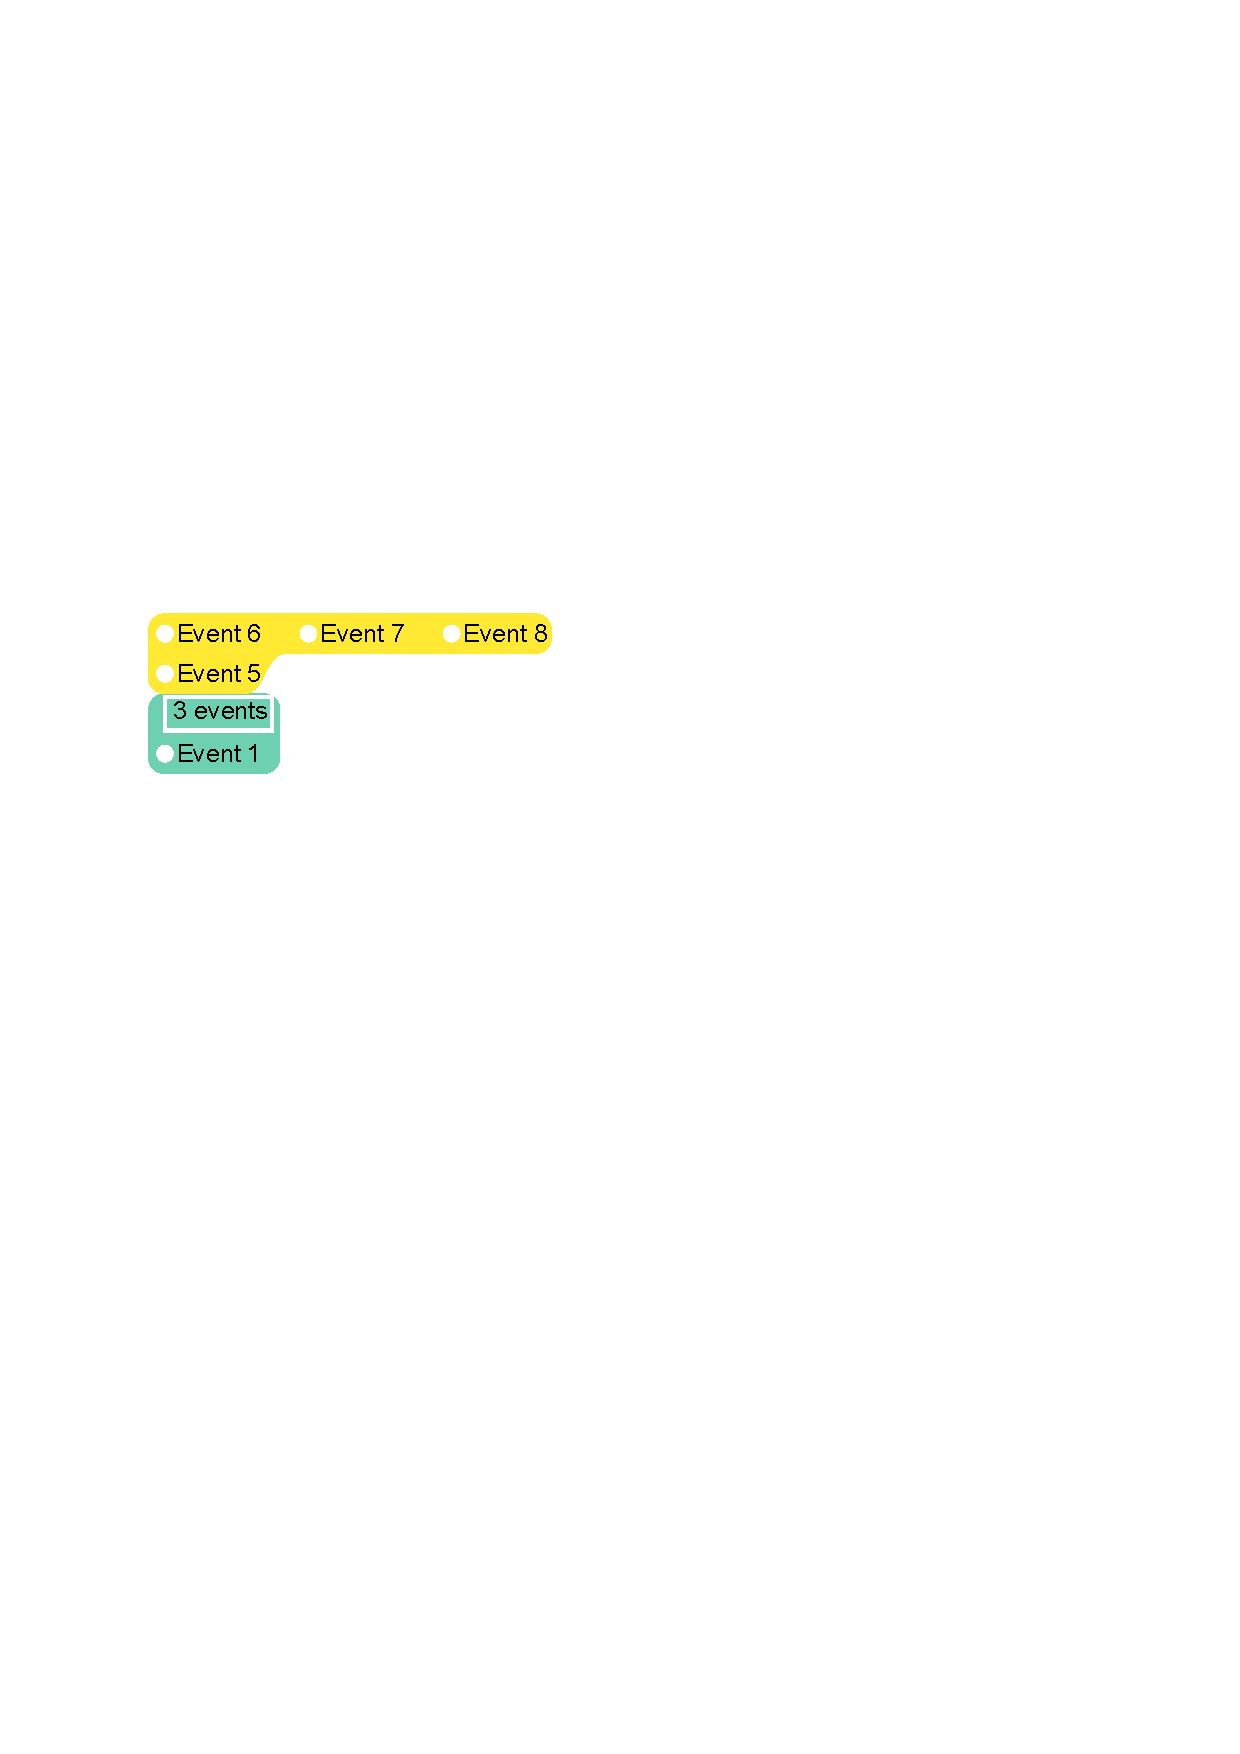
\includegraphics[width=.44\columnwidth]{figure11a}}
	\hfill
	\subcaptionbox{After: $\theta_{green}=\theta_{yellow}=0.5$.}{\label{fig:balancing2}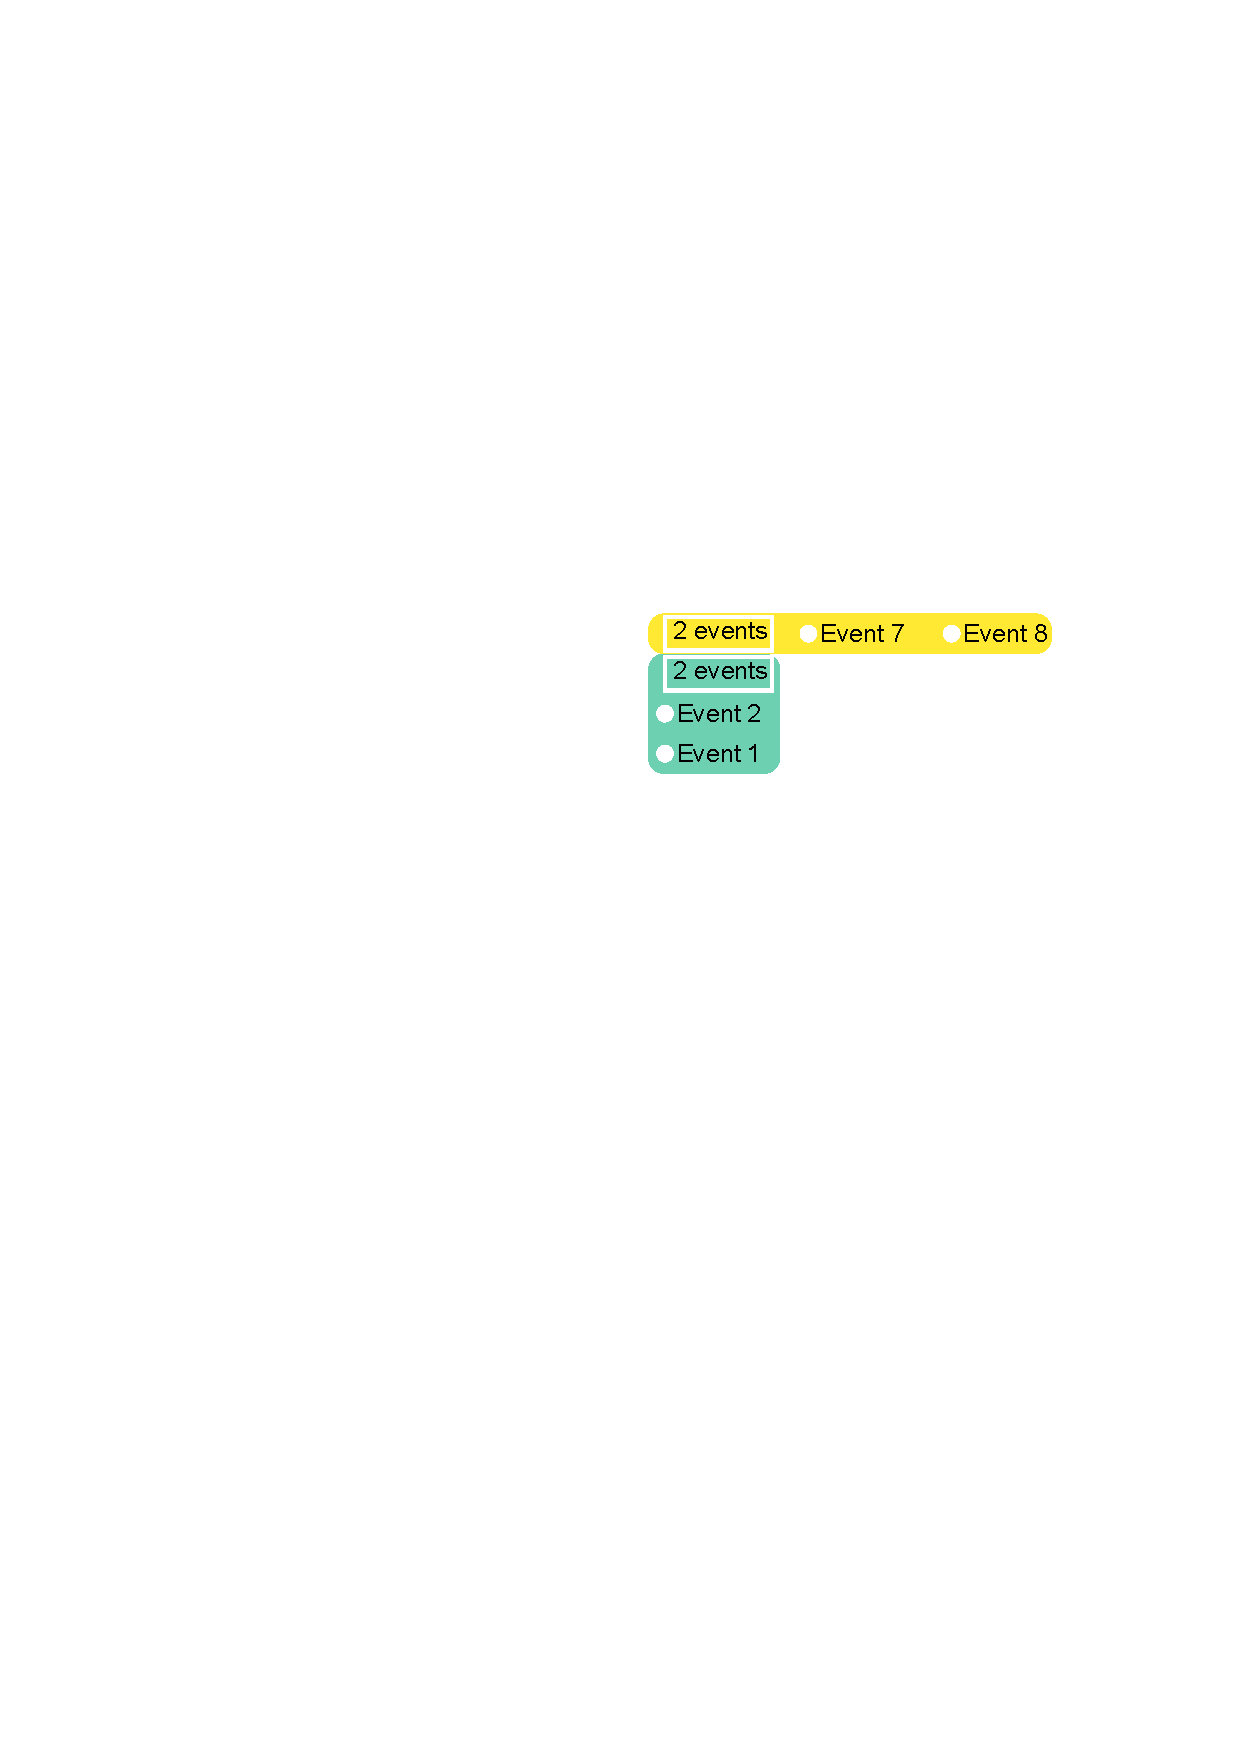
\includegraphics[width=.44\columnwidth]{figure11b}}
	\caption{Layers balancing.}
	\label{fig:balancing}
\end{figure}

\subsection{Scalability}
\label{sub:ts-scalability}
This section discusses the scalability of TimeSets: its capability, limitations and possible improvements. Aggregation enables TimeSets to visualize a large number of events. However, the visual representation of aggregated events is imperfect. For instance, two aggregates ``2 events'' and ``100 events'' are displayed exactly the same, except for the total number, whereas their sizes are largely different. We consider four options to address this issue as shown in \autoref{fig:ts-aggreate}.

\begin{figure}[!htb]
	\centering
	\subcaptionbox{No encoding.\label{fig:aggregate-0}}{
		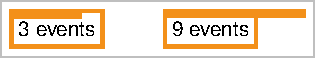
\includegraphics[width=.47\columnwidth]{figure12a}}
	\\
	\subcaptionbox{Each dot is an event at when it happens.\label{fig:aggregate-1}}{
		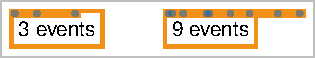
\includegraphics[width=.47\columnwidth]{figure12b}}
	\hfill
	\subcaptionbox{Scale with the width of the bounding rectangle.\label{fig:aggregate-2}}{
		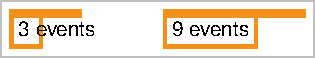
\includegraphics[width=.47\columnwidth]{figure12c}}
	\\
	\subcaptionbox{Color code the background of the bounding rectangle.\label{fig:aggregate-3}}{
		
\includegraphics[width=.47\columnwidth]{figure12d}}
	\hfill
	\subcaptionbox{Scale with the font size of the label.\label{fig:aggregate-4}}{
		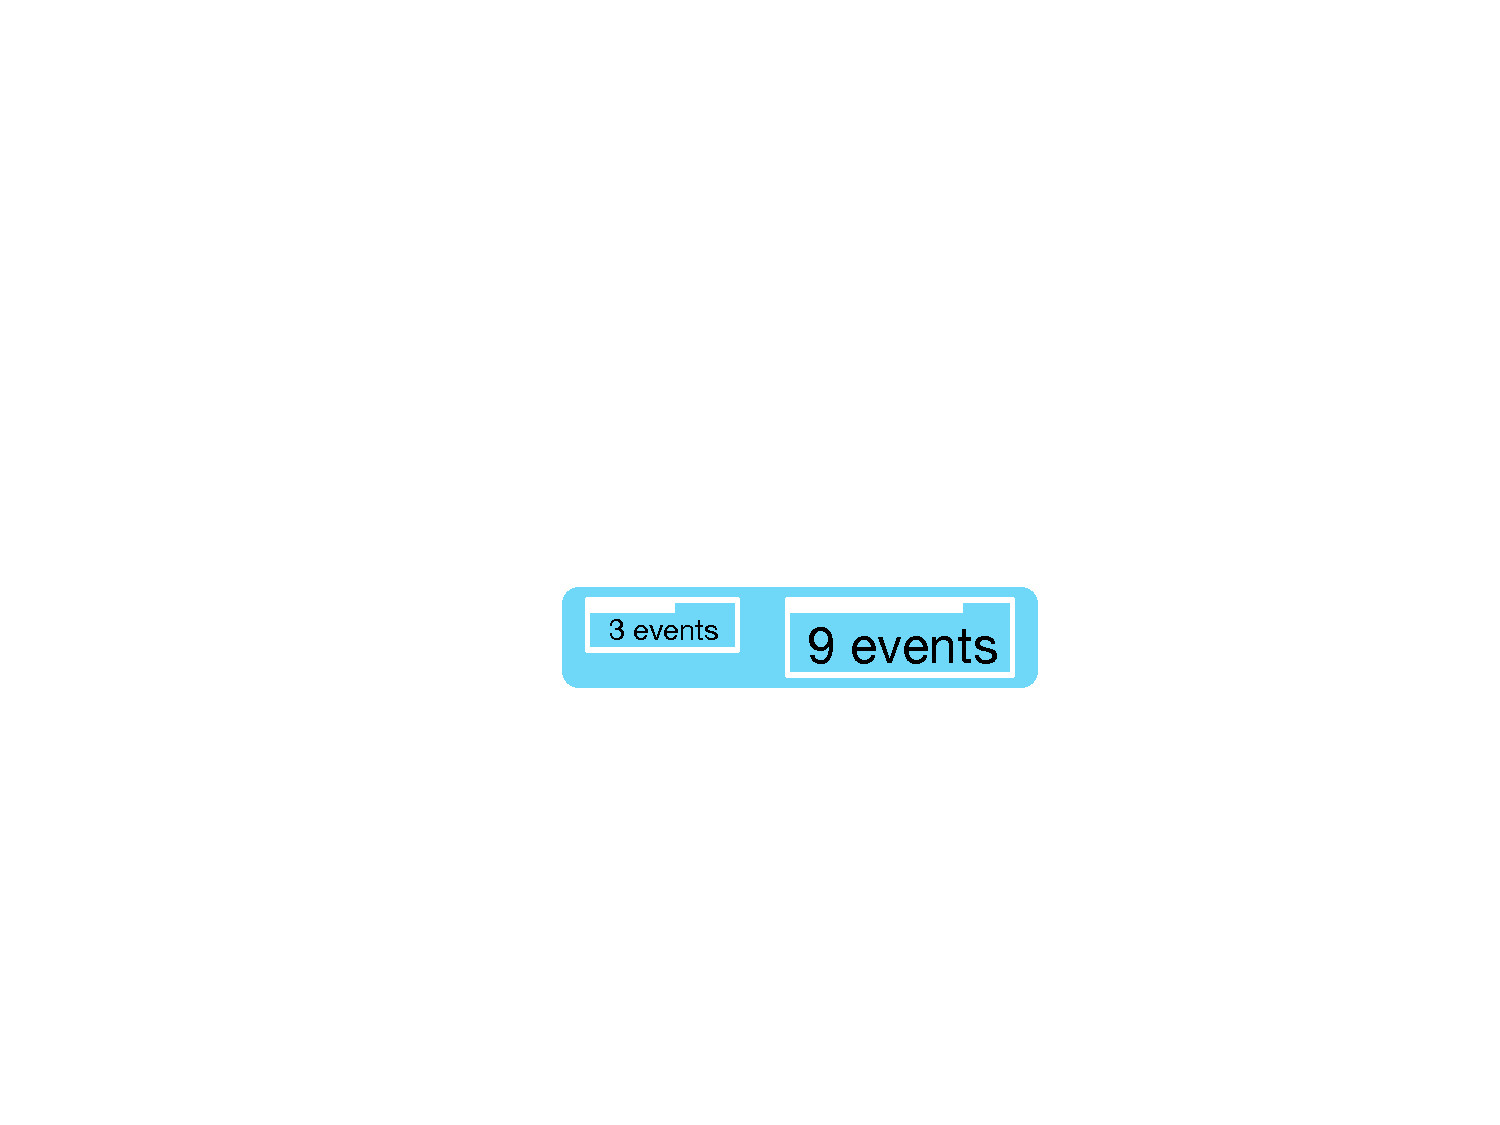
\includegraphics[width=.47\columnwidth]{figure12e}}
	\caption[Proposed visual representations of aggregates]{Proposed visual representations of aggregates emphasizing the number of its events.}
	\label{fig:ts-aggreate}
\end{figure}

The first option is to plot each individual event as a dot at when it happens (\autoref{fig:aggregate-1}). Besides providing a rough estimate of total count, this option also shows a temporal distribution of events. When events happen closely enough, their dots become overlapped, which makes it difficult to see the actual pattern. 

Second, the width of the aggregate rectangle can be scaled to indicate the number of events (\autoref{fig:aggregate-2}). The full width of an aggregate rectangle is typically small as the length of its text ``$N$ events''. Therefore, the difference of aggregate widths could be subtle and difficult to observe from an overview. 

Another option is to color code the background of the aggregate rectangle using luminance or intensity according to the number of events (\autoref{fig:aggregate-3}). However, when many aggregated events are displayed, their backgrounds could interfere with the set colors and distract users. 

The last option we propose is to scale the font size of the label based on the number of events (\autoref{fig:aggregate-4}). Currently, each event is completely located in one single row with uniform height. Scaling the heights of aggregated events will affect the layout algorithm.

The existing layout is suitable for a small timeline with a few hundreds of events or a detailed view where individual events are of high importance. \autoref{fig:citations} shows TimeSets with a medium-sized publication dataset: 200 articles spanning 15 years. TimeSets relies on color to distinguish sets, therefore the number of sets it can support is constrained by the number of colors that human can differentiate at the same time, which is about 12~\cite{Munzner2014}.
\section{Evaluation}

\subsection{Method}
% Overview of our method
We considered timeline visualizations that apply the two most powerful Gestalt principles of grouping to include in the evaluation. For \textit{proximity} principle, as discussed in the related work, LifeLines~\cite{Plaisant1996a} cannot show multi-set events, and storyline visualizations~\cite{Liu2013} only work for interval multi-set events. For \textit{uniform connectedness} principle, methods that connect all events belonging to the same set together without using a designated layout to reduce edge crossings such as tmViewer~\cite{Kumar1998} produce a cluttered visualization. To the best of our knowledge, there is no existing visualization that is designed to show multi-set relations and temporal information of events together. Therefore, rather than evaluating both the layout and the set visualization technique of TimeSets, we decided to focus only on the second one. We compared TimeSets with a set visualization technique that can apply on top of an existing timeline. We chose KelpFusion because among similar techniques, it has been shown to have the best performance in readability tasks in both accuracy and completion time~\cite{Meulemans2013}. We acknowledged that KelpFusion was not specifically designed to work with timelines. However, KelpFusion can work with any given layouts, and it is the best choice for this evaluation. We conducted a controlled experiment to compare TimeSets and KelpFusion. It followed a within-subject design; and accuracy, time and user preference were collected.
 
\subsubsection{Datasets}
We used generated data for the experiment to remove the possibility that participants might be distracted by their existing knowledge of scenarios. Only time-point events are used because KelpFusion needs a set of points as its input. The complexity of dataset was controlled by two parameters: the number of sets and the average number of events per set. Overall, half of the events were part of more than one set; this is the same ratio as in the CIA Leak case dataset. The details of the four levels of complexity used in the experiment are shown in Table~\ref{table:dataset}.

\begin{table}[ht]
\centering
\caption{Data Set Statistics}
\label{table:dataset}
\begin{tabular}{cccc}
	\toprule
	Complexity & \# sets & \# events & \# intersections \\ 
	\midrule
	Level 1 & 3 & 30 & 15 \\ 
	Level 2 & 3 & 45 & 23 \\ 
	Level 3 & 5 & 50 & 25 \\ 
	Level 4 & 5 & 75 & 38 \\ 
	\bottomrule
\end{tabular} 
\end{table}

We introduce three approaches to visualize intersections between more than two sets; however, evaluating all of them would triple the number of trials and make the experiment too long. We plan a separate experiment to study which method is the most effective as our future work. In this experiment, we only tested two-sets intersections and simple white circles are used for events' time indicators. 

Images of this dataset using the KelpFusion method were generously provided by the method's author. To avoid bias, our method also used static images instead of interactive visualizations. Colors for both methods were Qualitative Set 2 of ColorBrewer~\cite{Harrower2003}. KelpFusion does not have its own layout; therefore, our layout algorithm was used for both settings. Only one algorithm is used to prevent adding another factor to the experiment, which doubles the number of trials for participants. The traceability algorithm was chosen because reading comprehension is not required for the tasks. Figure~\ref{fig:evaluation} shows example images used in the experiment. 

\begin{figure}[ht]
	\centering
	\subcaptionbox{TimeSets.}{\label{fig:evaluation1}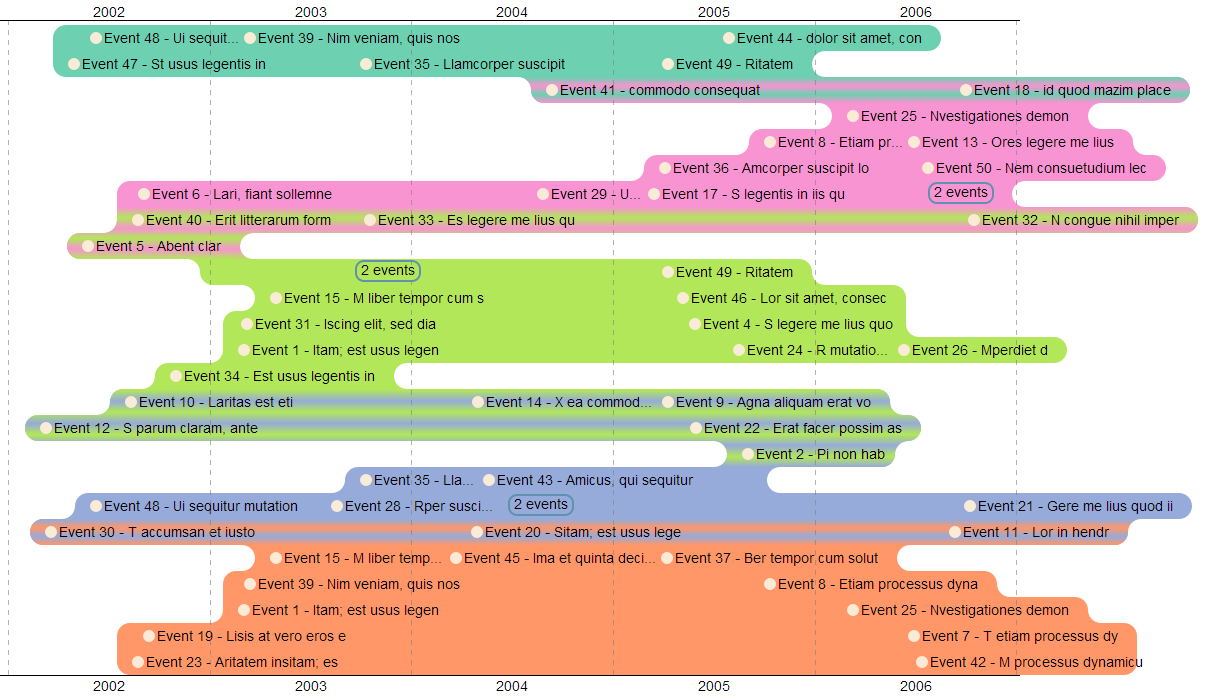
\includegraphics[width=\linewidth]{figure14a}}\\
	\subcaptionbox{KelpFusion.}{\label{fig:evaluation2}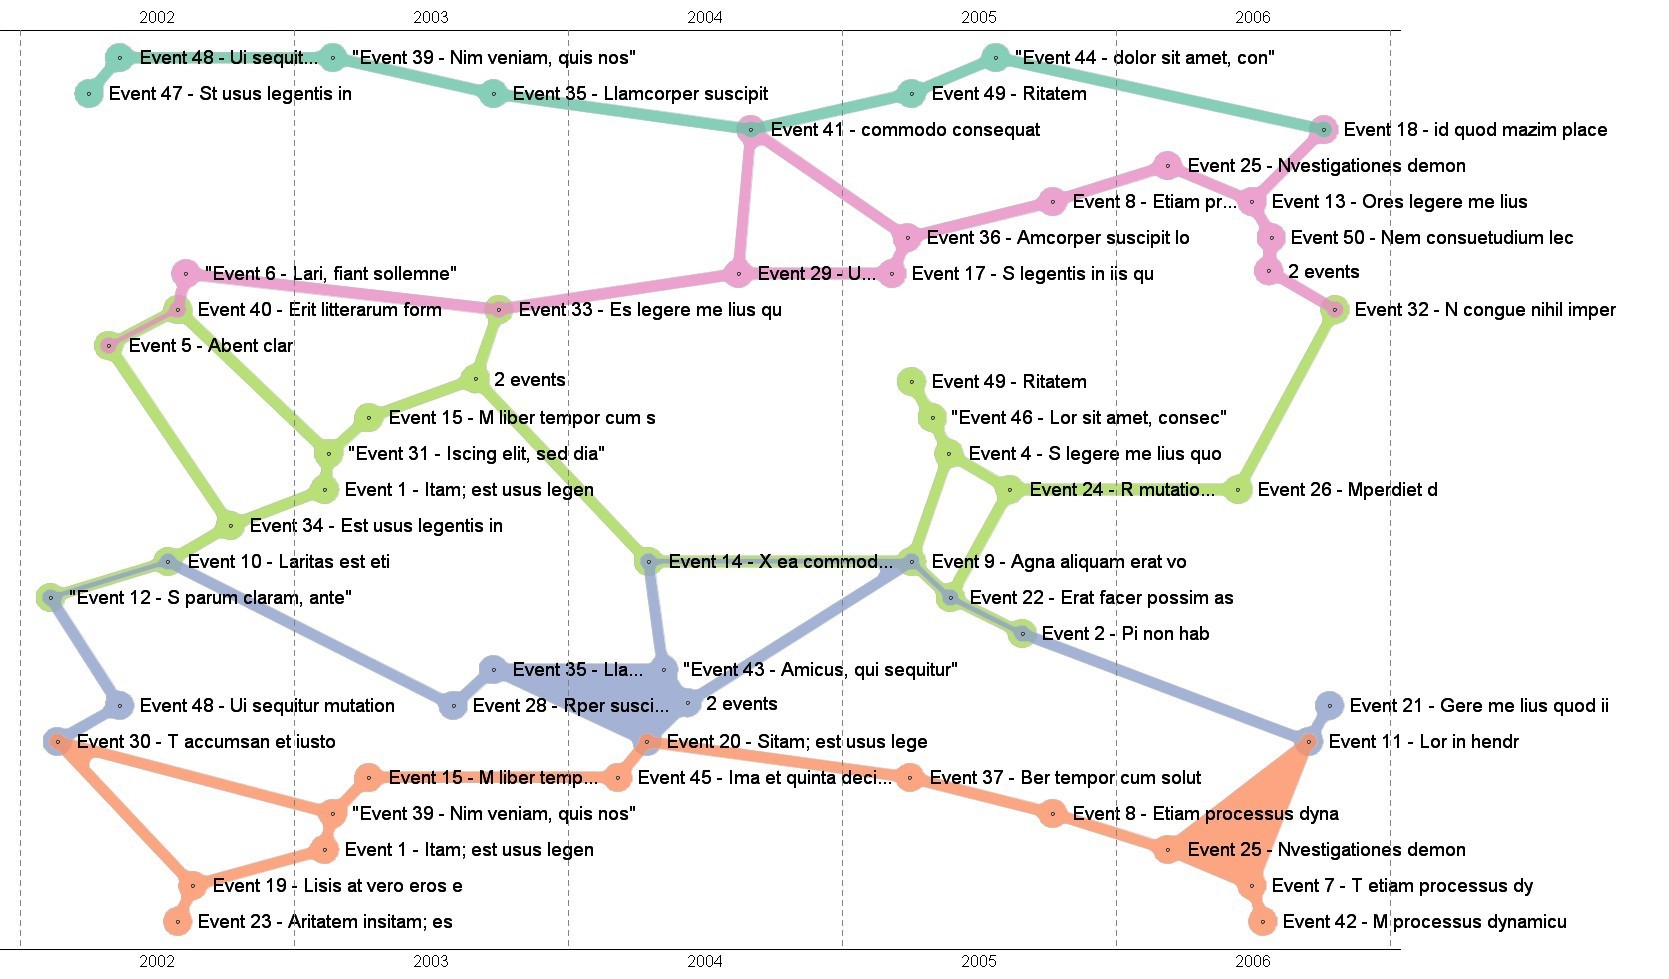
\includegraphics[width=\linewidth]{figure14b}}
	\caption{Example images used in the experiment.}
	\label{fig:evaluation}
\end{figure}

\subsubsection{Tasks} We followed the task design in the KelpFusion technique evaluation~\cite{Meulemans2013}, including estimation and precise comparison of set sizes, and counting the number of elements in a set. Two time-related tasks were added to evaluate the temporal aspect of the  visualization. Therefore, there are five tasks in total. We considered three categories of set readability tasks, relating to: the \textit{set} itself, the \textit{intersection} of two sets, and the \textit{difference} between two sets. However, it was impractical to include all 5 $\times$ 3 task types in the experiment. Therefore, we decided to use two tasks for the set only, two tasks for the intersection, and one task for the difference. Tasks together with examples are listed in Table~\ref{table:tasks}. Each participant would complete a total of 40 questions.

\begin{table}[ht]
\centering
\caption{Tasks used in our experiment}
\label{table:tasks}
\begin{tabular}{rl}
	\toprule
	Task & Example \\ 
	\midrule
	SetOverview & Roughly estimate which set has more events:  A or B \\&(please do \textbf{NOT} count the number of events)? \\		
 	IntersectionCompare & Which set pair shares more events: A\&B or C\&D\\&  (please count the number of events)? \\ 
 	DifferenceCount & How many events are there that belong to the set A \\&but not its neighboring sets? \\ 
 	SetBiggestYear & In which year does set A have the most events? \\ 
 	IntersectionPattern & During 2002--2004, what is the change pattern in the \\& number of  events shared by set A\&B?\\
	\bottomrule
\end{tabular} 
\end{table}


We use general questions to help preserve the external validity of the experiment. It is straightforward to convert them into context-sensitive questions. For example, the last task in the context of \textit{news media} can be written as ``what is the trend of news articles related to both science and fashion during the last 3 years?''. We chose to use multiple-choice answers to reduce the completion time, thus to allow the within-subject comparison to finish in a reasonable time. This reduces the possible effect of boredom or fatigue as confounding factors. It also removes the requirement to consider the typing speed of subjects when evaluating time taken to complete tasks.

\subsubsection{Participants and Apparatus} Thirty students (23 males, 7 females) voluntarily participated in the experiment. They came from various backgrounds including computing, law, and psychology. One participant was under 19, 16 participants were aged between 19--25, 12 were aged between 26--39, and one was aged between 40--60. All participants reported that they can distinguish all colors used in the experiment. Participants completed the experiment using a 23-inch monitor with a resolution of 1920 $\times$ 1080.

\subsubsection{Procedure} The study lasted approximately 45 minutes and consisted of two sessions (one for each visualization technique), followed by a questionnaire. At the beginning of each session, the visualization technique was explained, and participants were shown how to answer each question type using that method. This was followed by five practice questions to familiarize participants with the tasks and the experiment interface. Solutions and explanations were given for these practice questions to help them understand better.

We used two question sets with comparable difficulty and counterbalanced the order of the visualization techniques as well as the order of question sets to reduce learning effects. We fixed the order of task types and the order of difficulty in each type from simple to complex. For each task, the question and all the answer options were displayed without the visualization. Once participants finished reading, they clicked a button to reveal the figure, when the timing started. This is to reduce the affect of individual differences in reading and comprehension speed on the measured time. 

\subsection{Hypotheses}
\label{sec:hypotheses}

\begin{description}
	\item [H1.] TimeSets will have higher accuracy and shorter completion time for all tasks compared to KelpFusion. The colored set background in TimeSets can have a stronger sense of grouping than the line connection in KelpFusion, which may make the set-related tasks easier. Also, shared events are visually grouped in TimeSets, separating from the non-shared ones. This may help its performance in tasks related to shared events.
	
	\item [H2.] TimeSets will require less time for the SetOverview task than KelpFusion, but will be less accurate. The color background in TimeSets makes it easier to recognize a group. However, the set size is not a precise indicator of event number because it is also affected by the label lengths and the gap between events.
	
	\item [H3.] TimeSets will outperform KelpFusion in time and accuracy on both IntersectionCompare and IntersectionPattern tasks. In TimeSets, shared events are visually grouped in its own layer, whereas in KelpFusion, they are mixed with non-shared events, which may affect its performance for tasks involves share events.
	
	\item [H4.] TimeSets will outperform KelpFusion in the DifferenceCount task. Similar to the last hypothesis, in TimeSets, events not belonging to neighboring sets have their own layer with a unique background color, whereas in KelpFusion such events are mixed with the shared events. This can make this task easier with TimeSets.
	
	\item [H5.] KelpFusion will outperform TimeSets in the SetBiggestYear task. When looking at elements in each year, connected lines in KelpFusion make it easier to count, compared to TimeSets.
\end{description}

For user preference, we hypothesized that
\begin{description}
	\item [H6.] Participants will be more confident with TimeSets because it provides better visual support, especially in intersection and difference tasks.
	
	\item [H7.] TimeSets will be more aesthetically pleasing than KelpFusion with smooth curves and smooth color changes compared to straight lines and plain colors.
	
	\item [H8.] TimeSets will be less cluttered than KelpFusion because it uses simple shapes, while KelpFusion uses a combination of lines and areas.
	
	\item [H9.] TimeSets will provide a stronger sense of grouping than KelpFusion because it colors the entire background of the set.
\end{description}

\subsection{Results}
We used a repeated-measure analysis of variance (RM-ANOVA) to analyze the task accuracy and completion time. Accuracy is measured as the percentage of correct answers. The logarithm of completion time is used to normalize its skewed distribution.

\subsubsection{Accuracy}
Figure~\ref{fig:accuracy} shows the mean accuracy. The RM-ANOVA test revealed a significant main effect of visualization technique ($F(1,29)=4.99, p<.05$), showing that accuracy was significantly higher with TimeSets. There was also a significant main effect of task type ($F(4,116)=8.89, p<.00001$). No significant effect of the visualization $\times$ task interaction was found ($F(4,116)=1.85, p=.12$). Paired t-tests were conducted to investigate the performance difference for each task. A significant effect was found in three tasks: IntersectionCompare ($p<.05$), DifferenceCount ($p<.01$), and IntersectionPattern ($p<.05$), indicating TimeSets was significantly more accurate than KelpFusion in them. Only task DifferenceCount still had a significant effect with corrected p-value for multiple tests using Bonferroni correction.

\subsubsection{Time}
Figure~\ref{fig:time} shows the mean completion time. The RM-ANOVA test revealed no significant main effect of visualization technique ($F(1,29)=.05, p=.82$), indicating that the completion time for TimeSets ($M=23.87,SD=9.18$) and KelpFusion ($M=23.72,SD=11.38$) were not significantly different. There was a significant main effect of task type ($F(4,116)=23.80, p<10^{-12}$). The visualization $\times$ task interaction was also significant ($F(4,116)=3.23,p<.05$), indicating that difference in completion time due to visualization technique was significantly different across tasks. To further investigate this, a paired t-test for each task was conducted. Significant effects were found in DifferenceCount ($p<.01$), indicating TimeSets is significantly faster in this task, and SetBiggestYear ($p<.01$), indicating KelpFusion is significantly faster in this task. Both tasks still had a significant effect with corrected p-value for multiple tests using Bonferroni correction.

\begin{figure}[ht]
	\centering
	 {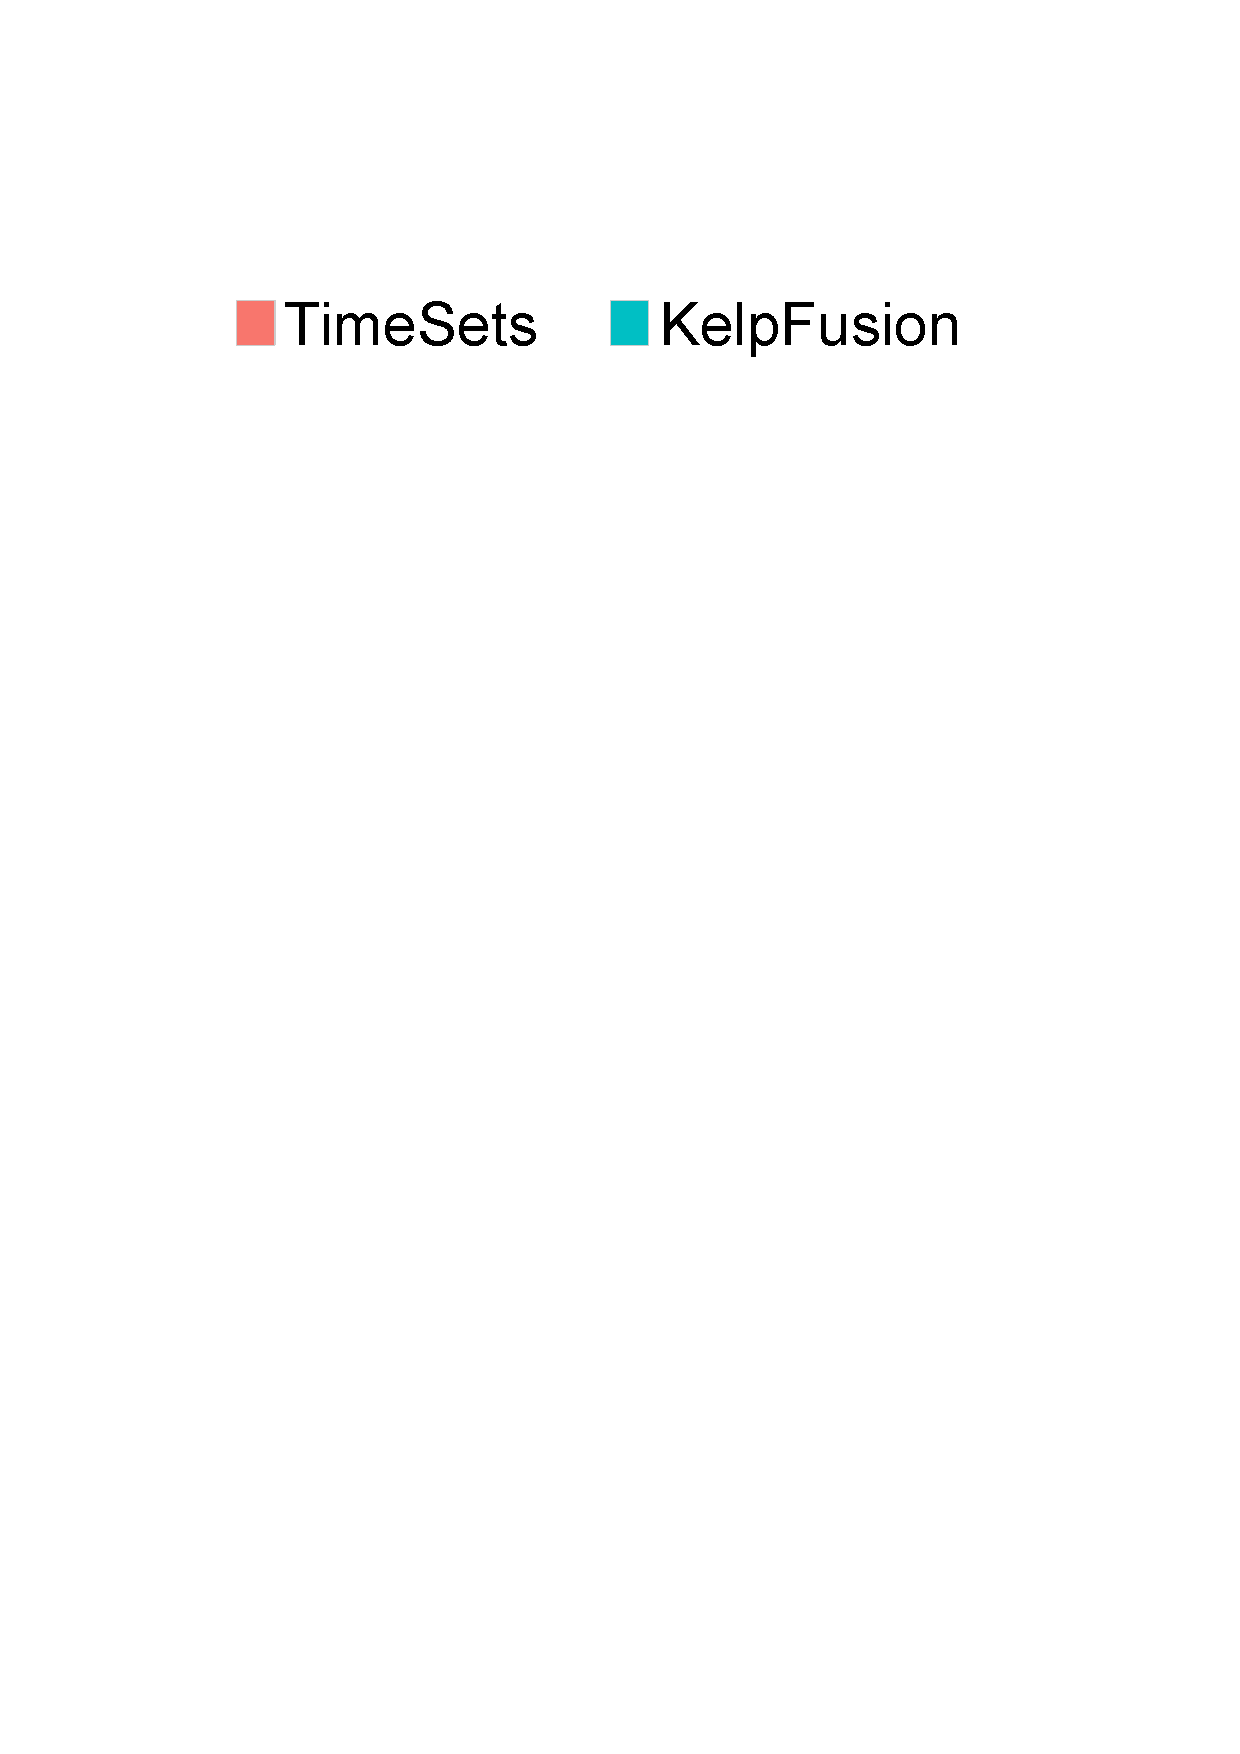
\includegraphics[width=.4\linewidth]{figure15a}} \\
	\subcaptionbox{Mean accuracy (in percentage).}{\label{fig:accuracy}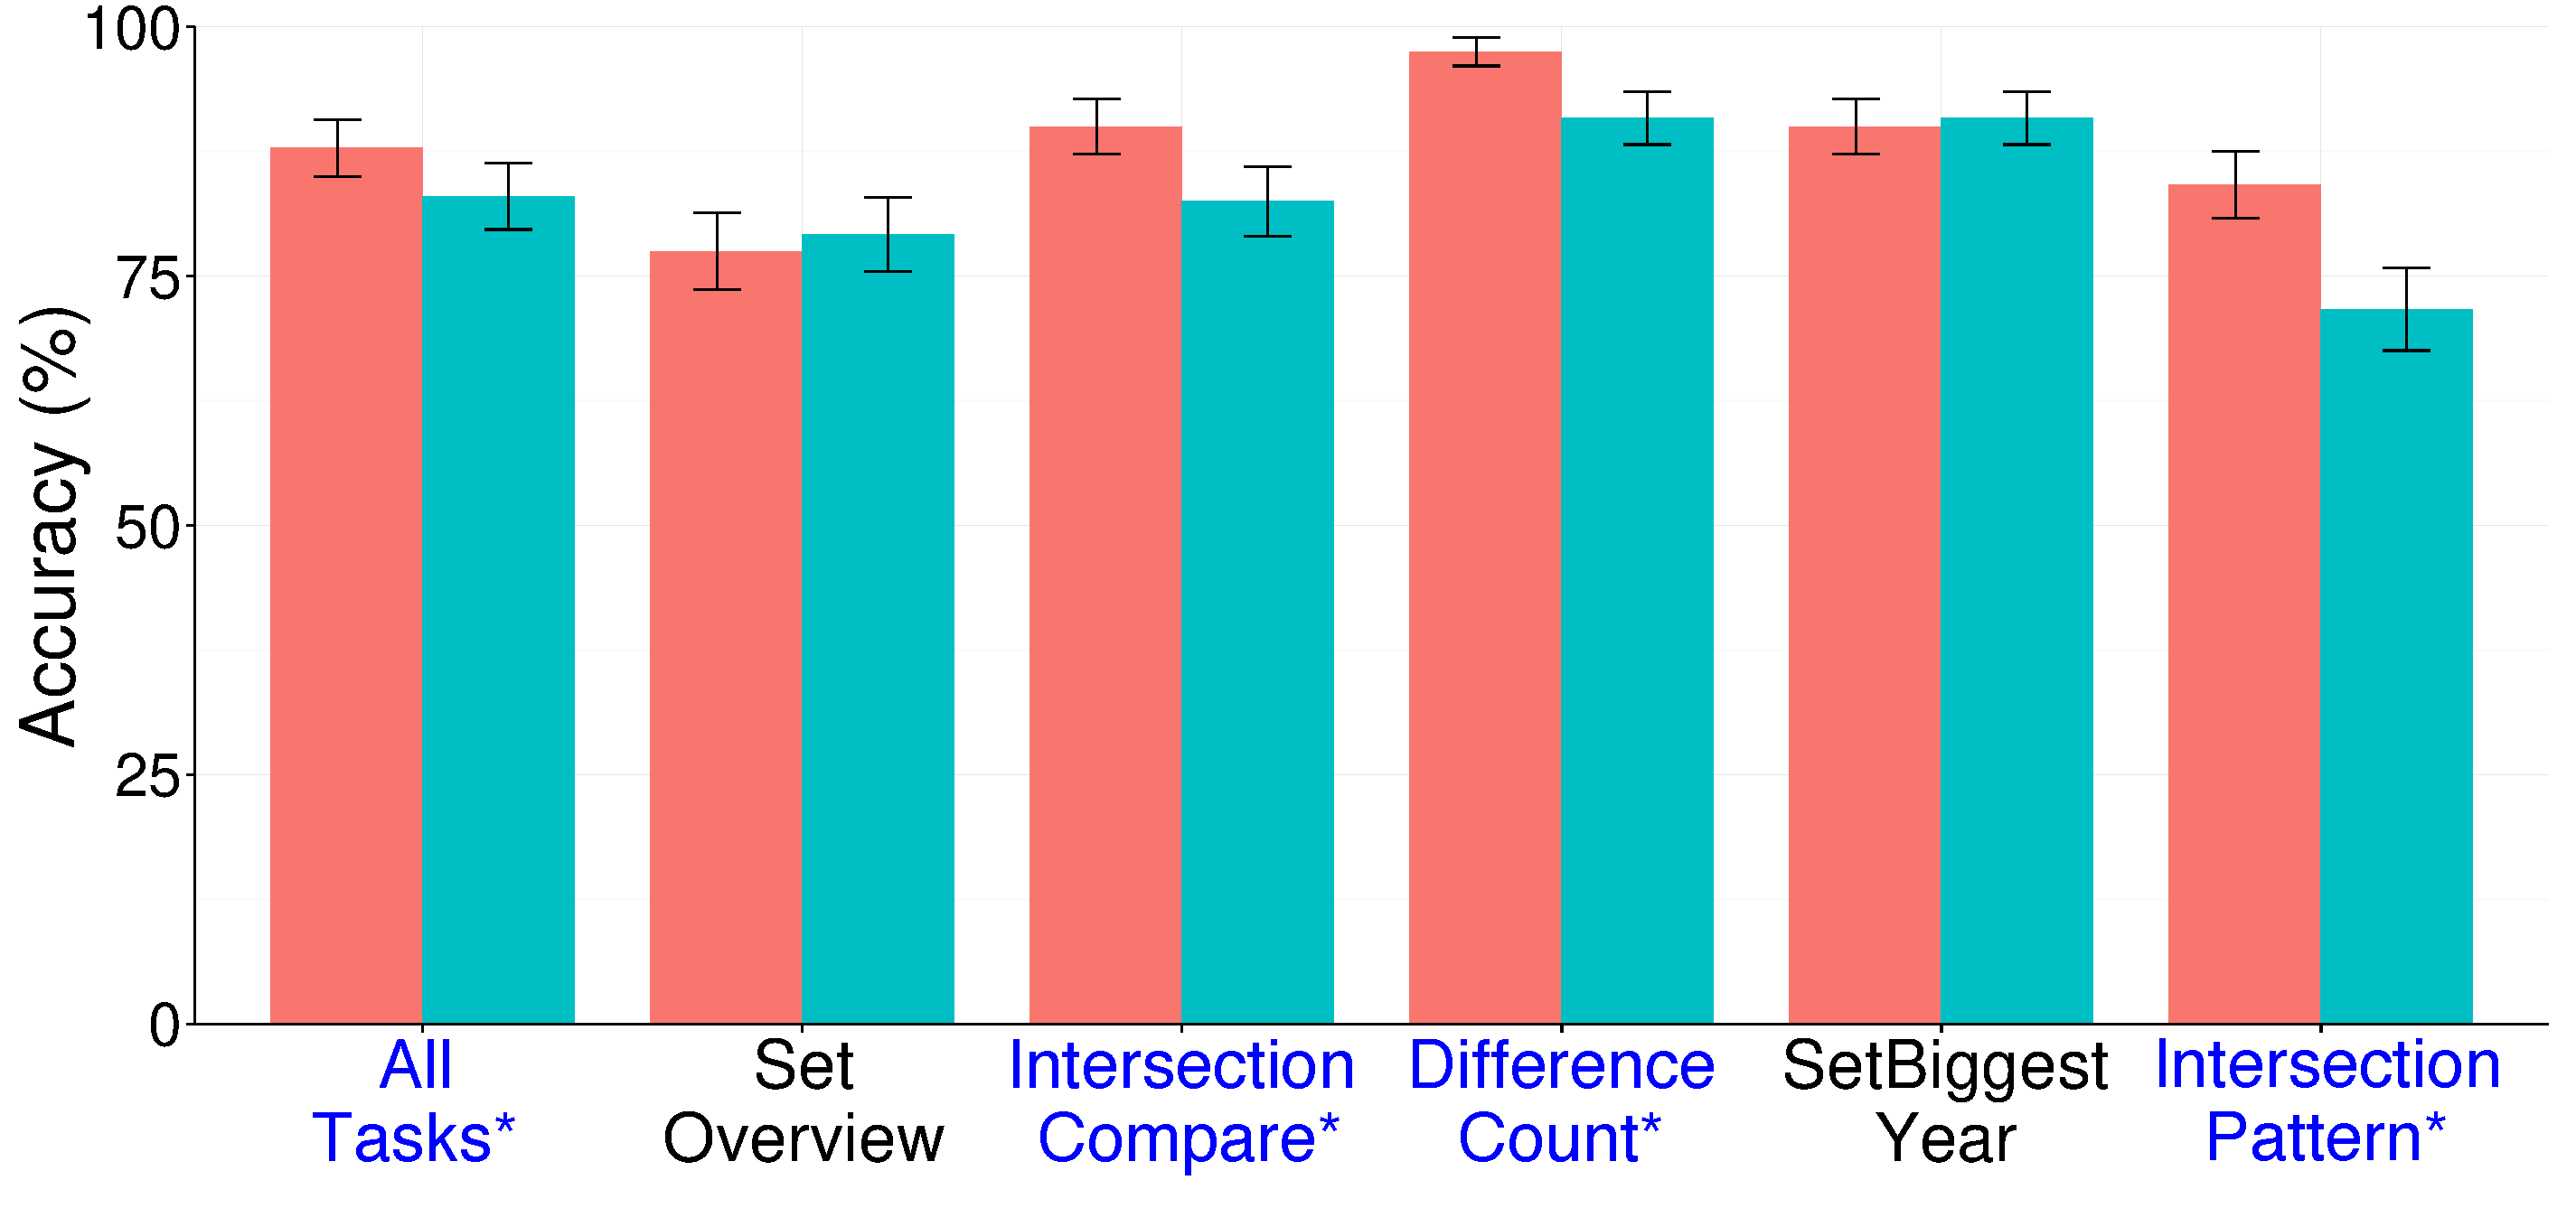
\includegraphics[width=.7\linewidth]{figure15b}}\\
	\subcaptionbox{Mean completion time (in seconds).}{\label{fig:time}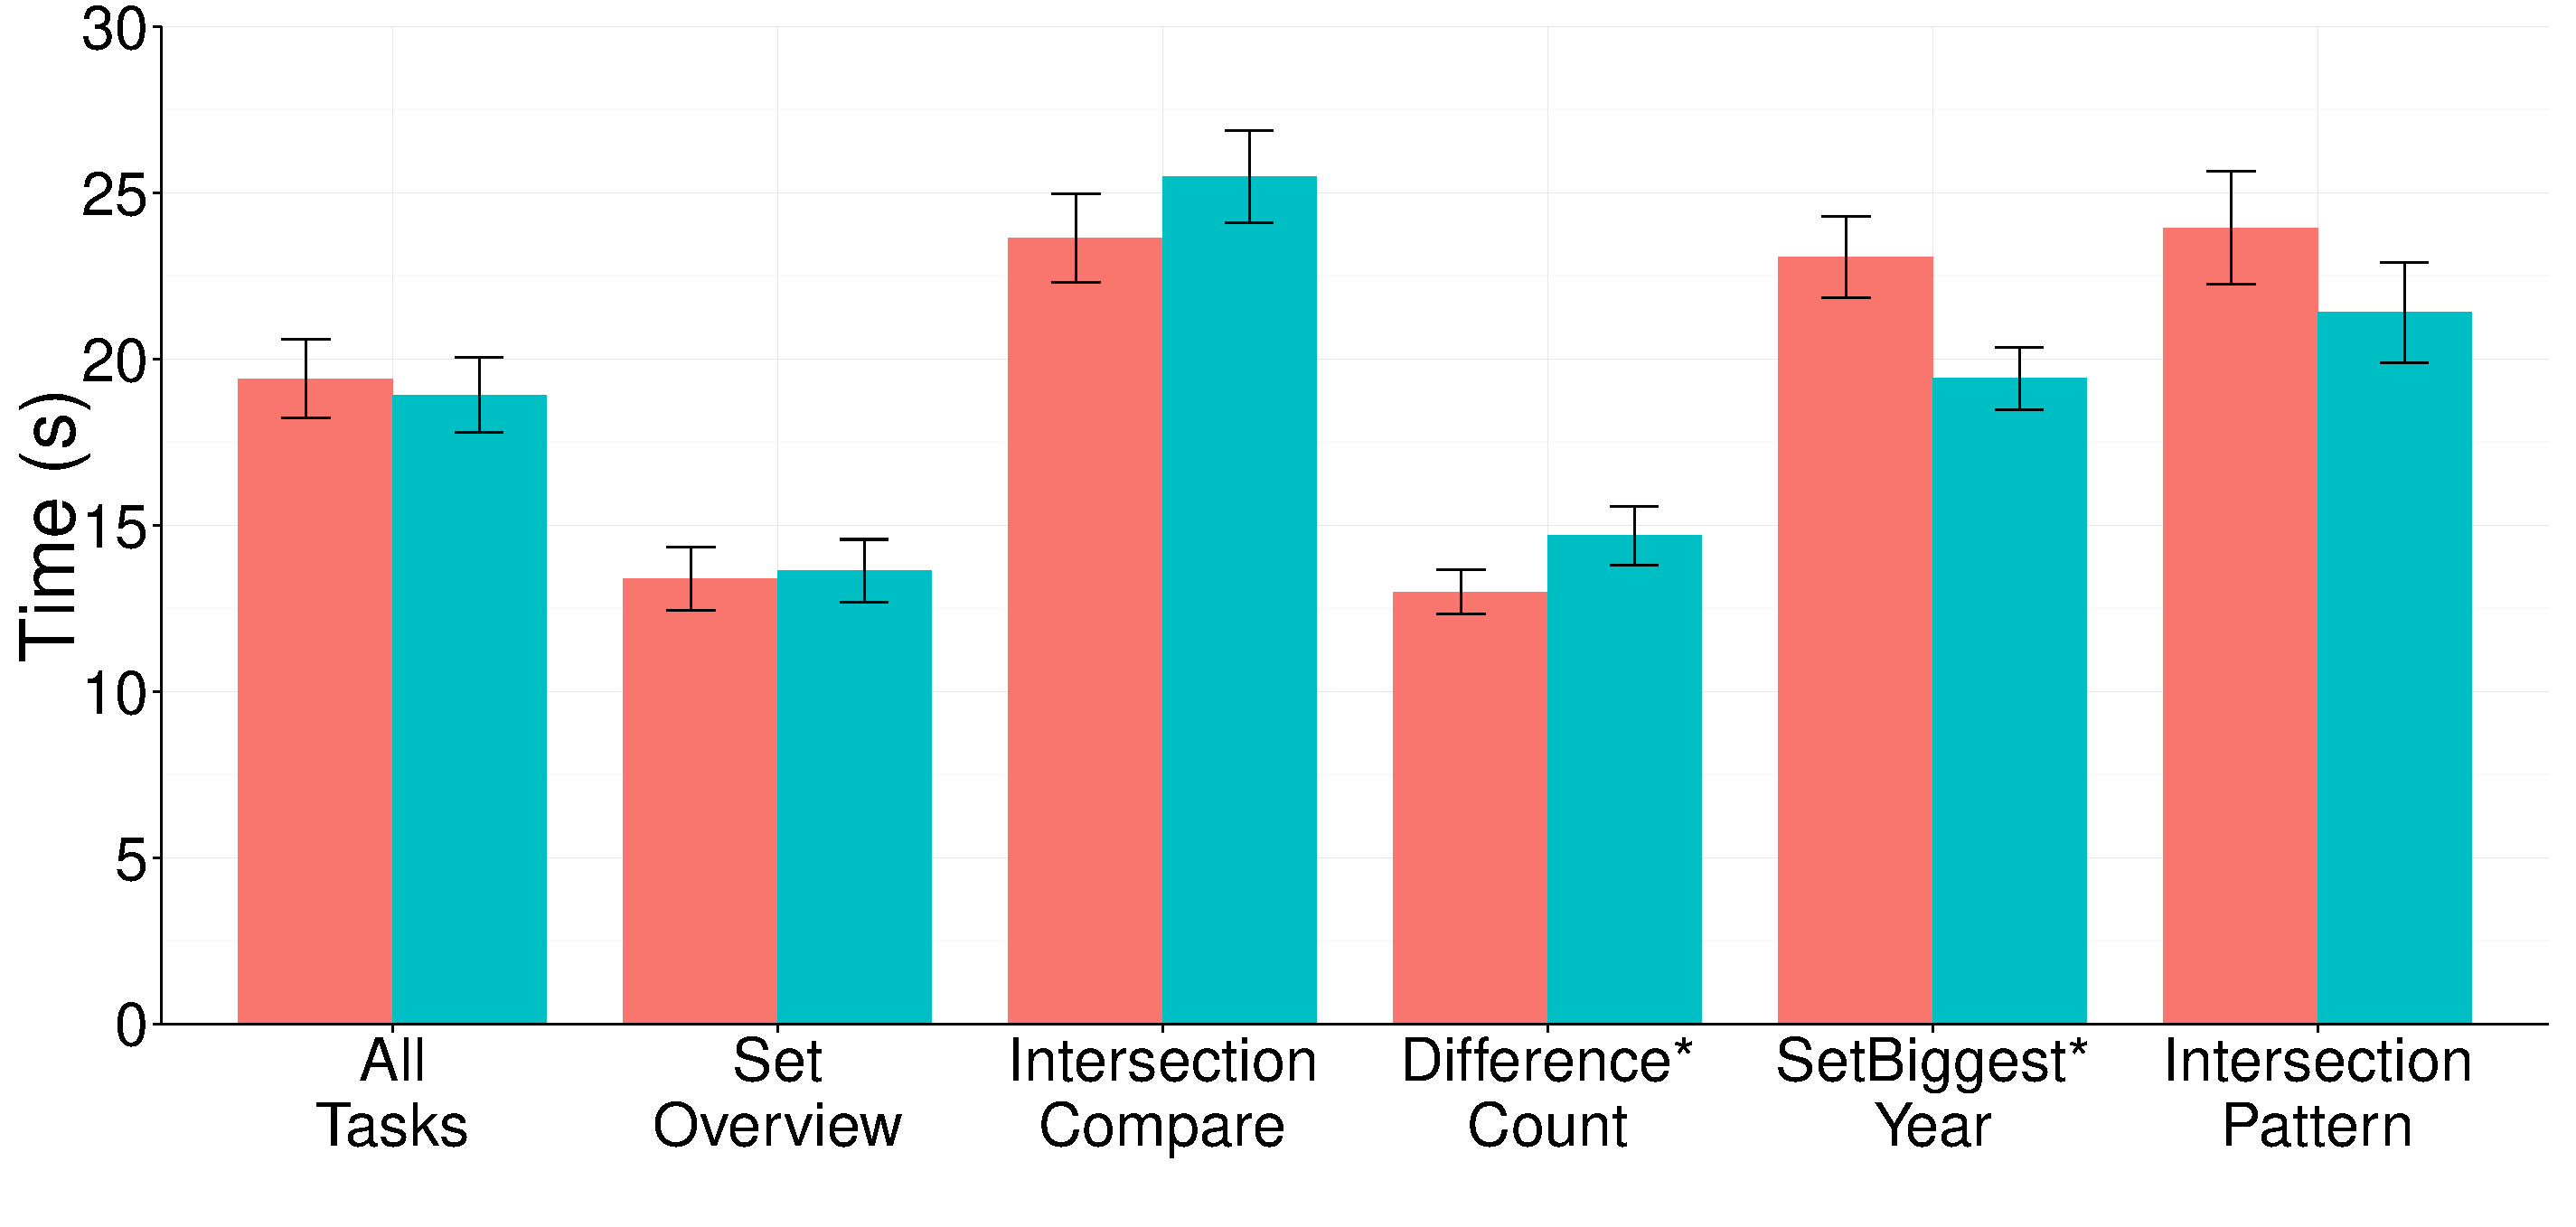
\includegraphics[width=.7\linewidth]{figure15c}}
	\caption{Mean accuracy and completion time of each tasks. Error bars show standard error. Significant effects are denoted by *.}
\end{figure}

\subsubsection{User Preference}
Participants were asked to rate both methods using a Likert scale 1 (worst) to 5 (best) after they completed all the tasks. Four questions were asked for each visualization technique: 
\begin{itemize}
	\item How confident were they in answering the questions? 
	\item How aesthetically pleasing were the visualizations? 
	\item How cluttered were the visualizations?
	\item How strong was the sense of grouping?
\end{itemize}
Figure~\ref{fig:ratings} shows the summary of user ratings. Fisher's exact tests found significant effects in all questions: Confidence ($p<.01$), Aesthetically Pleasing ($p<.01$), Not Cluttered ($p<.01$), and Sense of Grouping ($p<.0001$); indicating users preferred TimeSets to KelpFusion in those aspects.

\begin{figure}[ht]
	\centering
	\subcaptionbox{How confident were they in answering the questions?} {\label{fig:pref-confidence}
		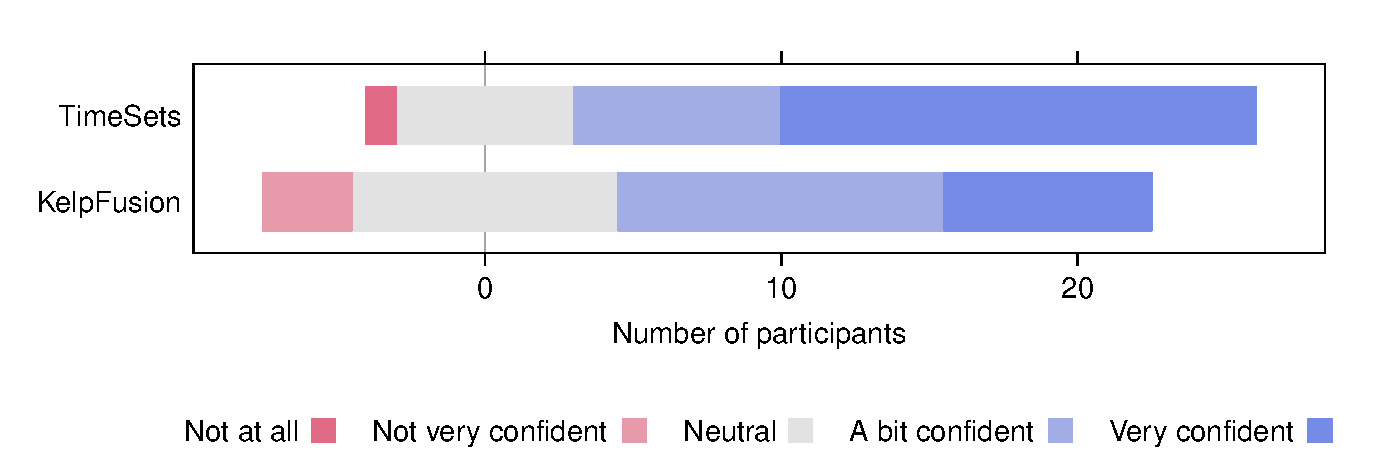
\includegraphics[width=.7\columnwidth]{figure16a}}
	\subcaptionbox{How aesthetically pleasing were the visualizations?}{\label{fig:pref-nice}
		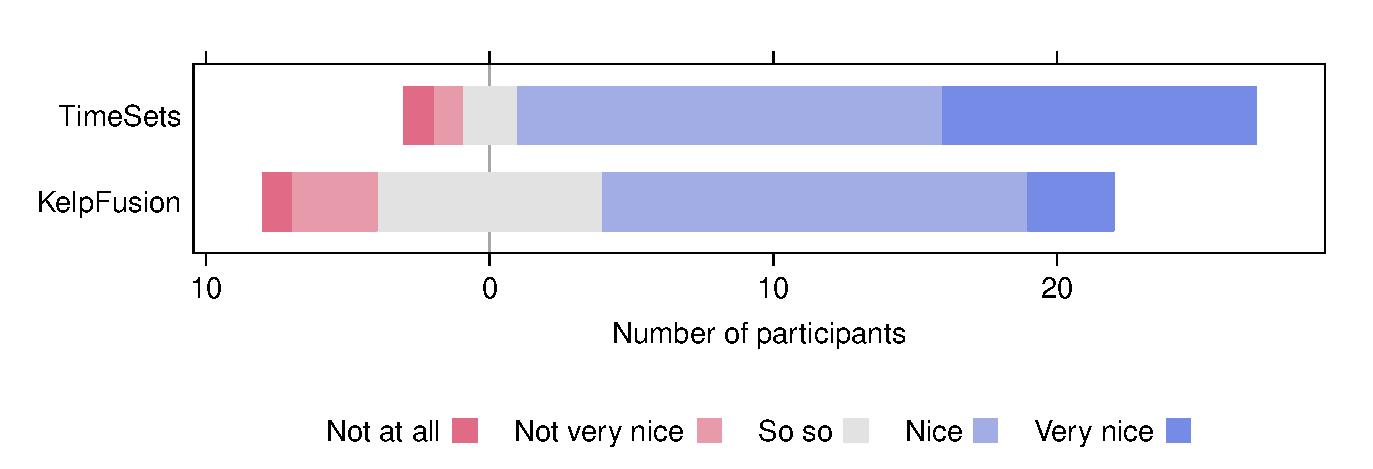
\includegraphics[width=.7\columnwidth]{figure16b}}
	\subcaptionbox{How cluttered were the visualizations?}{\label{fig:pref-read}
		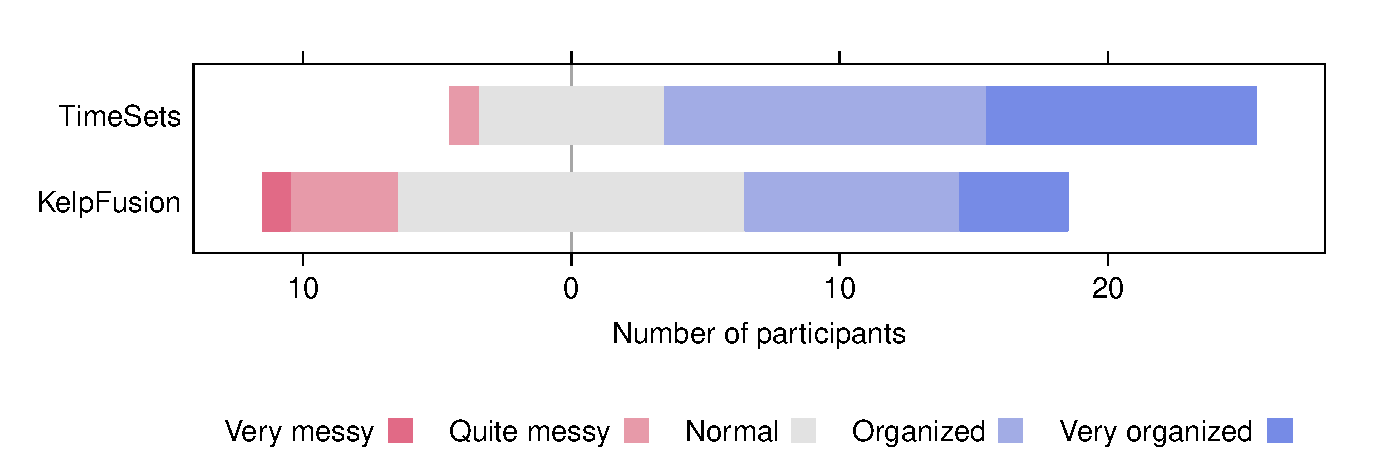
\includegraphics[width=.7\columnwidth]{figure16c}}
	\subcaptionbox{How strong was the sense of grouping?}{\label{fig:pref-group}
		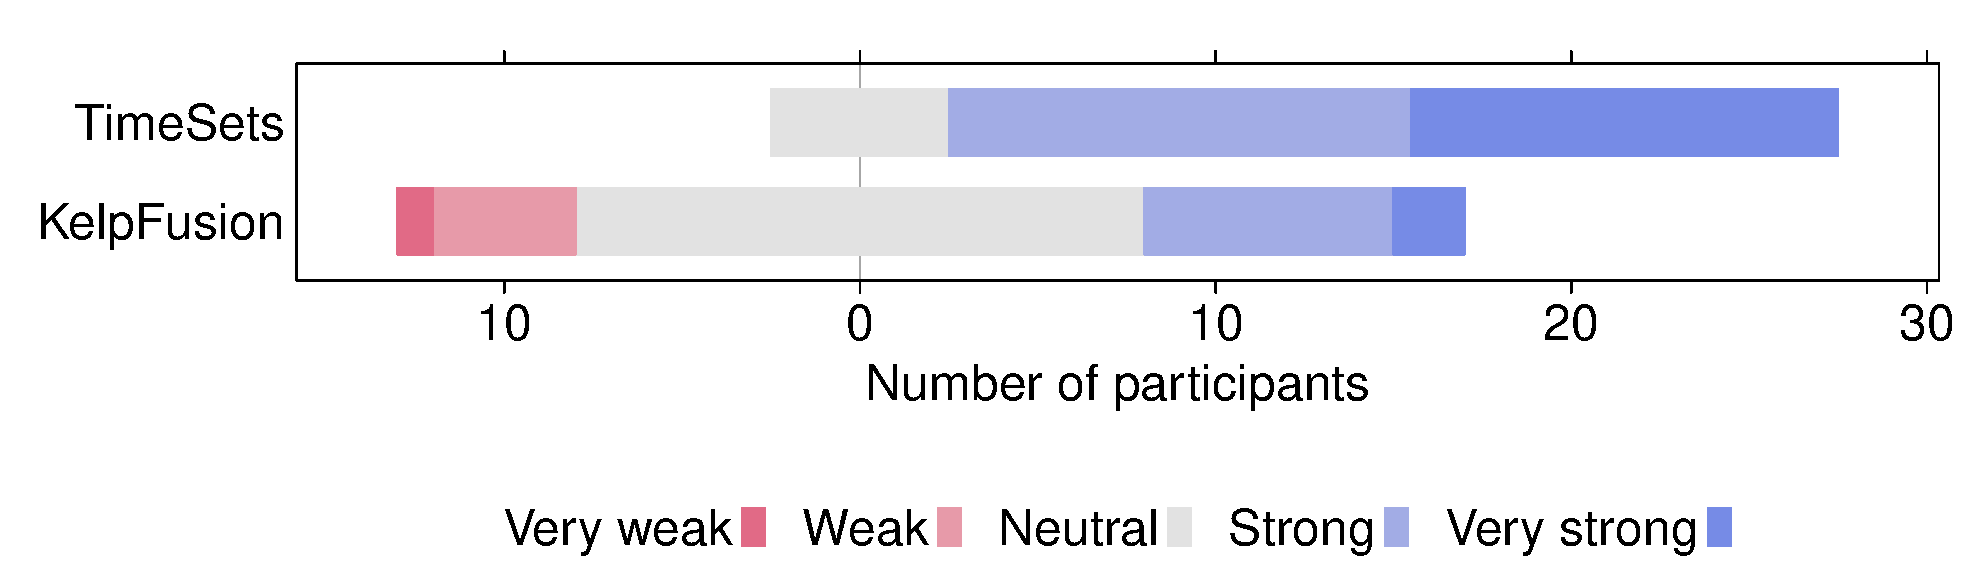
\includegraphics[width=.7\columnwidth]{figure16d}}
	\caption{Subjective user ratings of each technique for each question. Bar width represents the number of participants selected the corresponding option.}
	\label{fig:ratings}
\end{figure}

\subsection{Discussion}
The results show that in overall, TimeSets is more accurate than KelpFusion, but there is no significant difference in completion time. This partly agrees with hypothesis \textbf{H1}.

There was no significant effect of visualization technique on accuracy or completion time for the SetOverview task, which disagrees with hypothesis \textbf{H2}. The average accuracy of both methods is low, relatively to the other tasks in the experiment. Possible causes for TimeSets are discussed earlier in the hypothesis statement, and the edge length in KelpFusion, which is a prominent visual feature, is possibly not a good size indicator, either.

The results also show that for intersection tasks, TimeSets has higher accuracy than KelpFusion; however, their completion time performances are not significantly different. This partly confirms hypothesis \textbf{H3}. Shared events in TimeSets are highlighted by color gradient, and participants are less likely to miscount them, resulting in higher accuracy. In KelpFusion, shared events are horizontally aligned, because it shares the same layout as TimeSets. We observed that some participants tried to trace shared events this way, which is prone to missing events, thus similar speed but lower accuracy.

Hypothesis \textbf{H4}, about the DifferenceCount task, is supported by the results. Events that belong to a single set are clearly shown in TimeSets as a region with a single color background. This helps improve performance in both accuracy and completion time.

The results show that KelpFusion has faster completion time than TimeSets for the SetBiggestYear task, but there is no significant difference in accuracy. This partly agrees with hypothesis \textbf{H5}. The vertical lines used to denote year boundaries in this task may have helped, by splitting the visual area into columns. To solve the task, participants count the number of events in each column and pick the highest one. A KelpFusion visualization is quite similar to a network, and edges connecting events within each column can make counting easier. This may explain why participants counted faster with KelpFusion, but had the same accuracy as with TimeSets.

To visualize sets, Bubble Sets~\cite{Collins2009a} uses a similar metaphor as TimeSets -- filling the area of same-set events with a unique color. However, KelpFusion outperforms Bubble Sets~\cite{Meulemans2013}, while TimeSets outperforms KelpFusion in solving similar tasks. One possible explanation is that the irregular shapes generated using iso-contours in Bubble Sets make set memberships difficult to perceive. Also, the layout in TimeSets groups same-set events together, which allows participants to easier count or estimate. Another reason could be that the color gradient in TimeSets may be more effective than color blending in Bubble Sets for visualizing shared events.

The participants preferred TimeSets in all four questions: confidence, aesthetics, readability, and sense of grouping. This supports hypotheses \textbf{H6}, \textbf{H7}, \textbf{H8}, and \textbf{H9}. Half of the participants (15 out of 30) were more confident with TimeSets. Some of them commented that its set background made it easier to count events, especially for the intersections. Only four participants thought that they were more confident with KelpFusion (the other eleven thought they were at the same level of confidence). One said ``I can follow the links when counting, so I'm less likely to miss any''. Interestingly, three of these four participants actually had better accuracy with TimeSets. Half of the participants (15 out of 30) thought that TimeSets was more aesthetically pleasing than KelpFusion. Some of them said that they liked the curved boundaries and the smooth changing of colors. Only three participants favored KelpFusion. One of them commented that with TimeSets, his eyes were tired after looking at large areas with bright colors for a long time. More than half of the participants (17 out of 30) rated TimeSets as less cluttered than KelpFusion. One said ``TimeSets is more organized. I know event labels aren't important, but they seem easier to read.''. Three quarters of the participants (22 out of 30) agreed that TimeSets provided a stronger sense of grouping than KelpFusion. Many of them commented that KelpFusion figures looked more like a network than a group.
\section{Case Study 1: Publication Data}

TimeSets can be applied to domains requiring the understanding of temporal events including history, movies, publications, etc. Figure~\ref{fig:teaser} shows a timeline of the CIA leak case~\cite{CIA2007} covering both time-point and interval events happening from 2002 to 2007. In this section, we choose another domain, academic publications, to demonstrate TimeSets. A subset of 200 publications with the most citations is extracted from the IEEE InfoVis articles~\cite{Stasko2013}. Each publication is assigned one or many \textit{concepts} such as \textit{network} or \textit{evaluation}. We use concept as the set attribute to group publications. Figure~\ref{fig:citations} shows the visualization of this dataset. No aggregation is needed when producing the layout, only complete and trimmed labels are displayed in the visualization.

\begin{figure*}[ht]
\centering
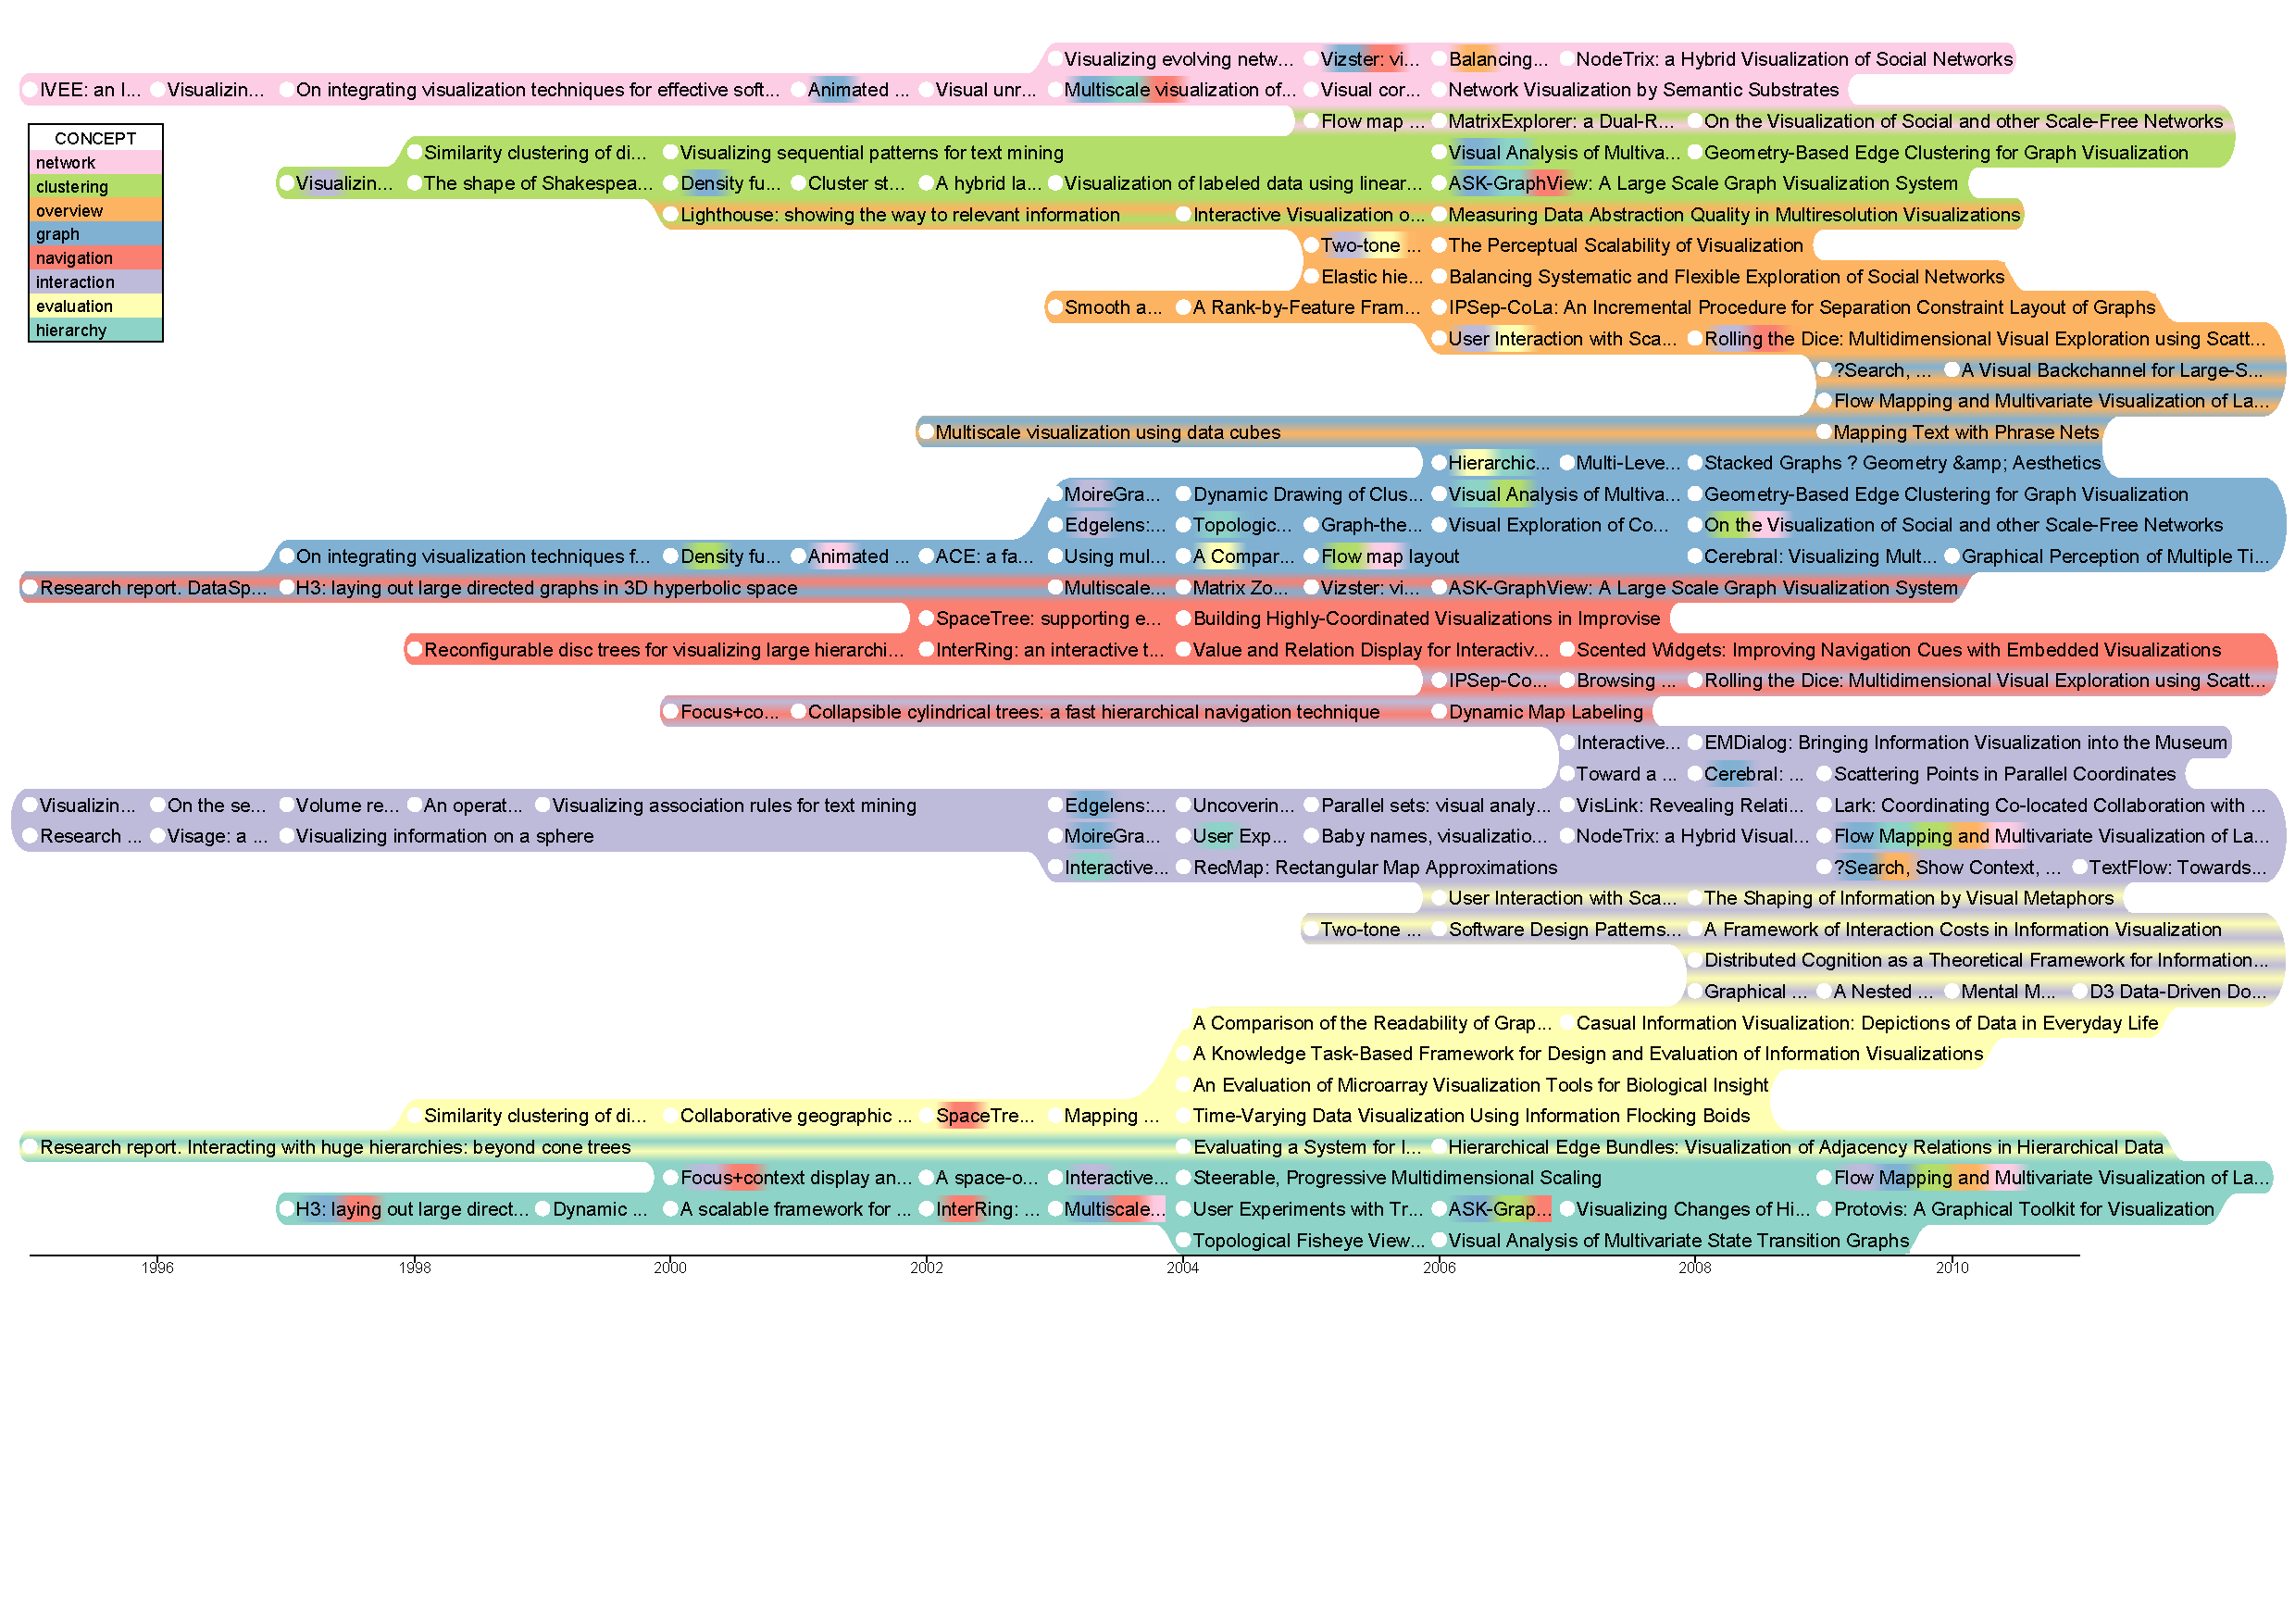
\includegraphics[width=\linewidth]{figure13}
\caption{TimeSets visualization of 200 publications with the most citations in the IEEE InfoVis conference from 1995 to 2013. Concepts are used to group publications and only eight concepts appearing most in those publications are shown (see the legend in the top left corner).}
\label{fig:citations}
\end{figure*}

TimeSets can show distribution of categorical data over time as in ThemeRiver~\cite{Havre2002}. A quick glance at the visualization brings us a surprise. There is much void space on the left as opposed to a very dense area on the right indicating that there are many more highly cited papers published in the last ten years of the dataset than in the first ten years. This trend also holds for individual concepts. Each colored band starts with a single row and increases its height towards the end of the timeline. This observation is in contrast with the common thought: papers published in a longer time would have more citations. One possible explanation is that the IEEE InfoVis conference accepts more papers over time -- in the dataset, there are 18 articles in 1995 while 37 articles in 2013. Another reason could be that publications in the last ten years are really of high quality.

TimeSets cannot show all intersections among sets; however,  its layout maximizes the number of shared elements between two neighboring sets. As a result, the visible intersections usually have the most elements among all intersection. In the visualization, the most notable gradient area is the intersection between yellow and purple sets implying that there are many excellent papers focusing on both \textit{evaluation} and \textit{interaction}. Another observation at the top of the visualization with three concepts: \textit{network}, \textit{clustering} and \textit{overview} with clustering is in between the other two. This is expected because clustering techniques are important in visualizing large networks or getting the overview of a large dataset.

In this figure, TimeSets uses the color gradient method to show full memberships of multi-set elements. For instance, inside the pink band (\textit{network} papers), there are quite a few small blue gradients (\textit{graph} papers). This is sensible because the closeness between these two concepts and they may often appear together in a paper. Another interesting observation is at the bottom band -- \textit{hierarchy}. The last paper ``Flow Mapping and Multivariate Visualization...'' includes five concepts: \textit{hierarchy} (blue background) and \textit{interaction}, \textit{graph}, \textit{overview} and \textit{network} (small gradients).
\section{Case Study 1: Intelligence Analysis}
\label{sub:ts-vast}
This case study explores how TimeSets supports intelligence analysis, the domain for which it is specifically designed. We integrated TimeSets into the visual analytics system SAVI~\cite{Xu2014} and used it to participate in the IEEE VAST Challenge 2014~\footnote{\url{http://www.vacommunity.org/VAST+Challenge+2014}}. Participants were given a synthetic dataset and asked to identify suspicious activities within that dataset. The particular mini challenge that SAVI involved was about a fictitious company where several employees had been missing. Participants had to collect and analyze streaming tweets in order to identify five \emph{interesting events} before presenting hypotheses and evidence about the disappearance of those employees. With the help of TimeSets, we won an award in Mini Challenge 3. Next, we describe the SAVI interface and how TimeSets contributes to make sense of temporal relationships in the data.

SAVI consists of five linked views (\autoref{fig:ts-savi}). To provide an overview of the dataset, a continuous histogram (\autoref{fig:ts-savi}A) shows the frequency of tweets over time (from 5pm to 9:30pm for this dataset). The histogram can provide initial cues for further investigation such as frequency peaks indicating that interesting events were happening around that time. Selecting the first peak (between 6:30pm to 7pm) makes the corresponding tweets to be displayed in the TimeSets view (\autoref{fig:ts-savi}C), allowing us to quickly read through those tweets and discover that there was a fire at the ``Dancing Dolphin Apartment''.

\begin{figure}
	\centering
	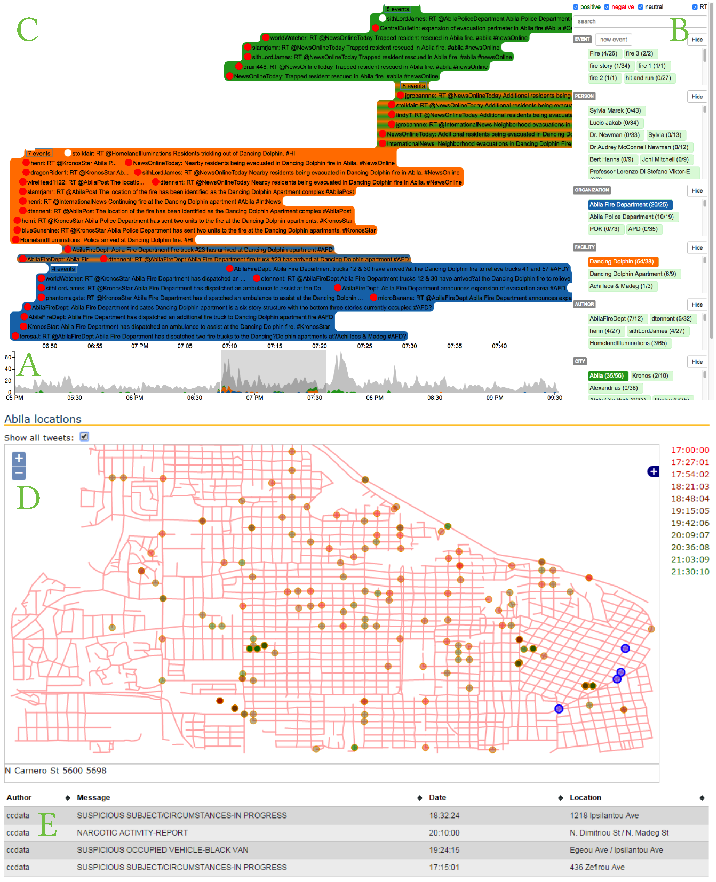
\includegraphics[width=\linewidth]{savi}
	\caption[SAVI interface]{SAVI interface. \textbf{A}: Histogram showing the distribution of tweets. \textbf{B}: Extracted named entities organized by type. \textbf{C}: TimeSets displaying selected tweets. \textbf{D}: Map showing tweets with available geolocation. \textbf{E}: Details of tweets selected in the map.}
	\label{fig:ts-savi}
\end{figure}

\autoref{fig:ts-savi}B displays named entities identified from the tweets and organized by entity type. Initially, entities from the entire dataset are shown, but they are updated according to the selected tweets. This view provides an overview of the main keywords mentioned in those tweets. Both the histogram and the entity collection act as filters. Within the previously selected time range, choosing the three most frequent entities (``Dancing Dolphin'', ``Abila Fire Department'' and ``Abila'') limits the tweets in TimeSets to only those containing at least one of the three keywords. TimeSets uses the entities as \emph{sets}, allowing us to quickly examine the story related to both individual and group of entities over time.

The map view (\autoref{fig:ts-savi}D) shows selected tweets with available geolocation information. Each tweet is displayed as a dot at its location and color-coded by its timestamp. These dots can be selected to reveal their detailed information as shown in \autoref{fig:ts-savi}E. TimeSets and other linked views enable us to explore temporal and spatial events.

Besides supporting data exploration, TimeSets can also help present discovered stories, which are interesting events or narratives in this case (\autoref{fig:ts-interesting-event}). An event is described as a sequence of related tweets organized in a chronological order. During the analysis, we create potential events and add tweets into one or multiple of them. As a result, TimeSets allows us to present an event together with its key elements. Also, visualizing many events simultaneously could reveal tweets that belong to multiple of them, which suggests further exploration to understand their relationship.

\begin{figure}
	\centering
	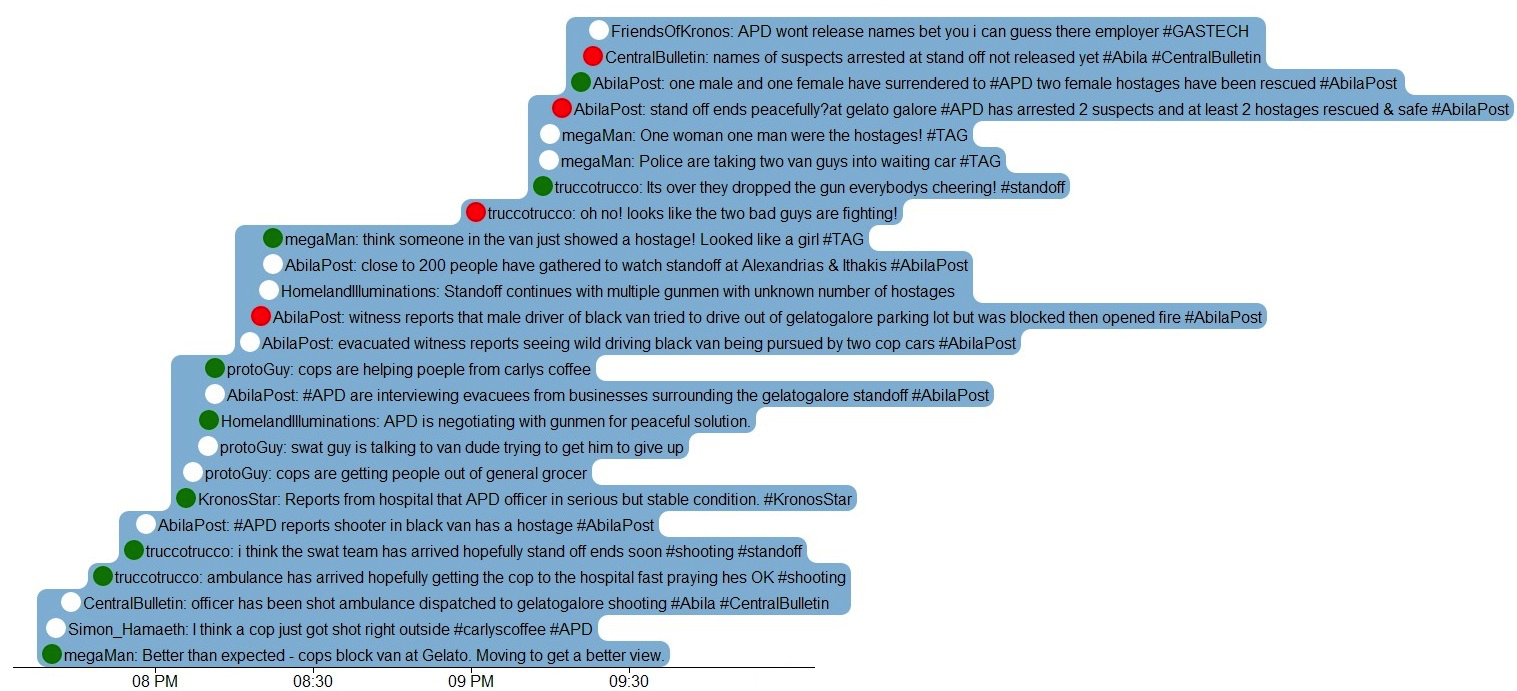
\includegraphics[width=\linewidth]{interesting-event}
	\caption{TimeSets for constructing and presenting an interesting event.}
	\label{fig:ts-interesting-event}
\end{figure}

In this case study, we show that TimeSets can be used effectively in supporting intelligence analysis through an application for a VAST Challenge entry. It was integrated into a visual analytics system (SAVI) for spatial-temporal analysis. TimeSets was applied to make sense of tweets in both temporal order and topical categories. It was also used to construct and present interesting stories. In other words, TimeSets showed its flexibility and usefulness of  mapping \emph{set} to different attributes for different purposes.
\section{Chapter Summary}
This chapter introduces TimeSets to enable users to explore complex temporal relationships by effectively representing both temporal and categorical provenance data. It groups temporal events vertically with colored backgrounds according to their set memberships, and uses colored gradient backgrounds for shared ones. Narrative construction was identified as an important user requirement in intelligence analysis, elicited in the previous chapter. Compared to SchemaLine, TimeSets enables analysts to explore and construct more complex, possibly related narratives. It also achieves a higher scalability through visual representations of events at different levels of detail.

TimeSets was designed to support sensemaking in intelligence analysis; however, it shows a much wider application. We demonstrated that it can be used to make sense of publication data and to visualize a number of different types of \emph{events} besides user annotations such as articles, news and tweets. For lower level tasks such as readability, TimeSets was shown to be significantly more accurate than KelpFusison, and the participants preferred TimeSets for aesthetics.

The major limitation of TimeSets is that it only shows intersections between vertically neighboring sets, which only accounts for a small portion of all possible combinations of intersections. The set ordering algorithm to maximize the number of shared events and interaction to reorder sets partially helped address this issue. Future research can focus on increasing the number of visible intersections, prioritizing more important intersections based on some metrics, and providing an overview of all intersections to suggest further exploration. Currently, duplicated events can only be discovered when mouse hovering. A better visual hint without making the visualization too much cluttered could be useful. We propose different techniques to encode multi-set memberships and to represent aggregated events. However, formal evaluations should be conducted to examine which options are the most effective.

SchemaLine and TimeSets allow users to externalize their sensemaking processes, construct and refine complex temporal frames to consolidate their thoughts. After being able to understand how things happened in a particular order, it is essential to understand their rationale. The next chapter will investigate how to design visualizations of analytic provenance data to enable users to explore such reasoning relationship.



%The contribution: TimeSets
%\begin{itemize}
%	\item Clearly shows the events within a set over time and their relationships with other sets.
%	\item Dynamically adjusts the level of details of each event to suit the amount of information and display estate.
%	\item Uses color gradient backgrounds for events belonging to multiple sets and curved set outlines to emphasize its grouping.
%\end{itemize}
%
%\section{Visual Design}
%
%\subsection{Event}
%Figure~\ref{fig:event-representation} shows examples these different visual representation of events.
%
%\begin{figure}[!htb]
%	\centering
%	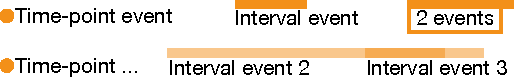
\includegraphics{figure2}\caption{Visual representations of events. Top row, left to right: a complete time-point event, a trimmed time-point event, and a aggregate of 10 events. Bottom row, left to right: an interval event, and two overlapping interval events.}
%	\label{fig:event-representation}
%\end{figure}
%
%\subsection{Set}
%\subsubsection{Design Overview}
%We use two most effective Gestalt's principles of grouping in our design: \emph{proximity} and \emph{uniform connectedness}. Events belonging to the same set are located close together, and the background of an entire set is colored to make its events visually connected.
%
%Spatial grouping is achieved through vertical positioning because the horizontal position of each event is already fixed by its temporal information. Figure~\ref{fig:layering} shows an example of a layering for three sets.
%
%\begin{figure}[!htb]
%	\centering
%	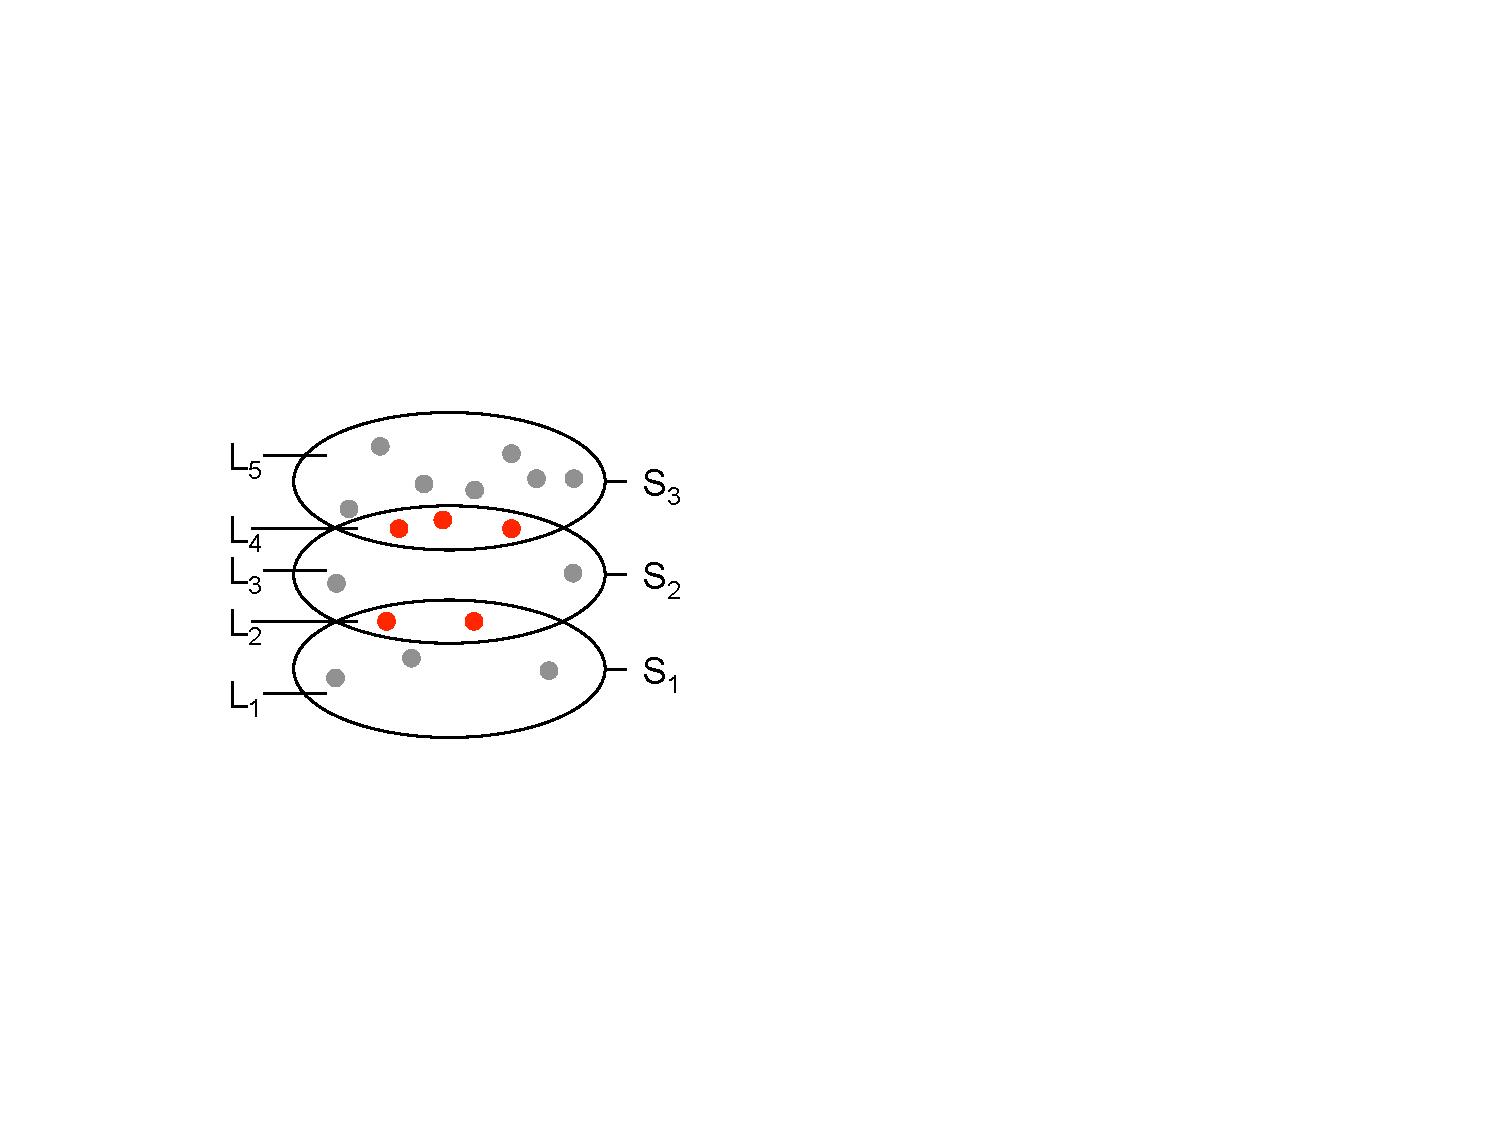
\includegraphics[width=.5\columnwidth]{figure3}
%	\caption{Layering for three sets $S_1$, $S_2$, and $S_3$. $L_2$ includes events shared by $S_1$ and $S_2$, and $L_4$ includes events shared by $S_2$ and $S_3$. Shared events are shown in red. $S_2$ consists of events in three layers $L_2$, $L_3$, and $L_4$.}
%	\label{fig:layering}
%\end{figure}
%
%Discuss design choices for visualizing shared events between two non-neighboring sets (Figure~\ref{fig:layering-compare})
%
%\begin{figure}[!htb]
%	\centering
%	\subcaptionbox{Shared events are only located in the green set, and connected to the orange set.\label{fig:layering-1}}[.47\columnwidth]
%	{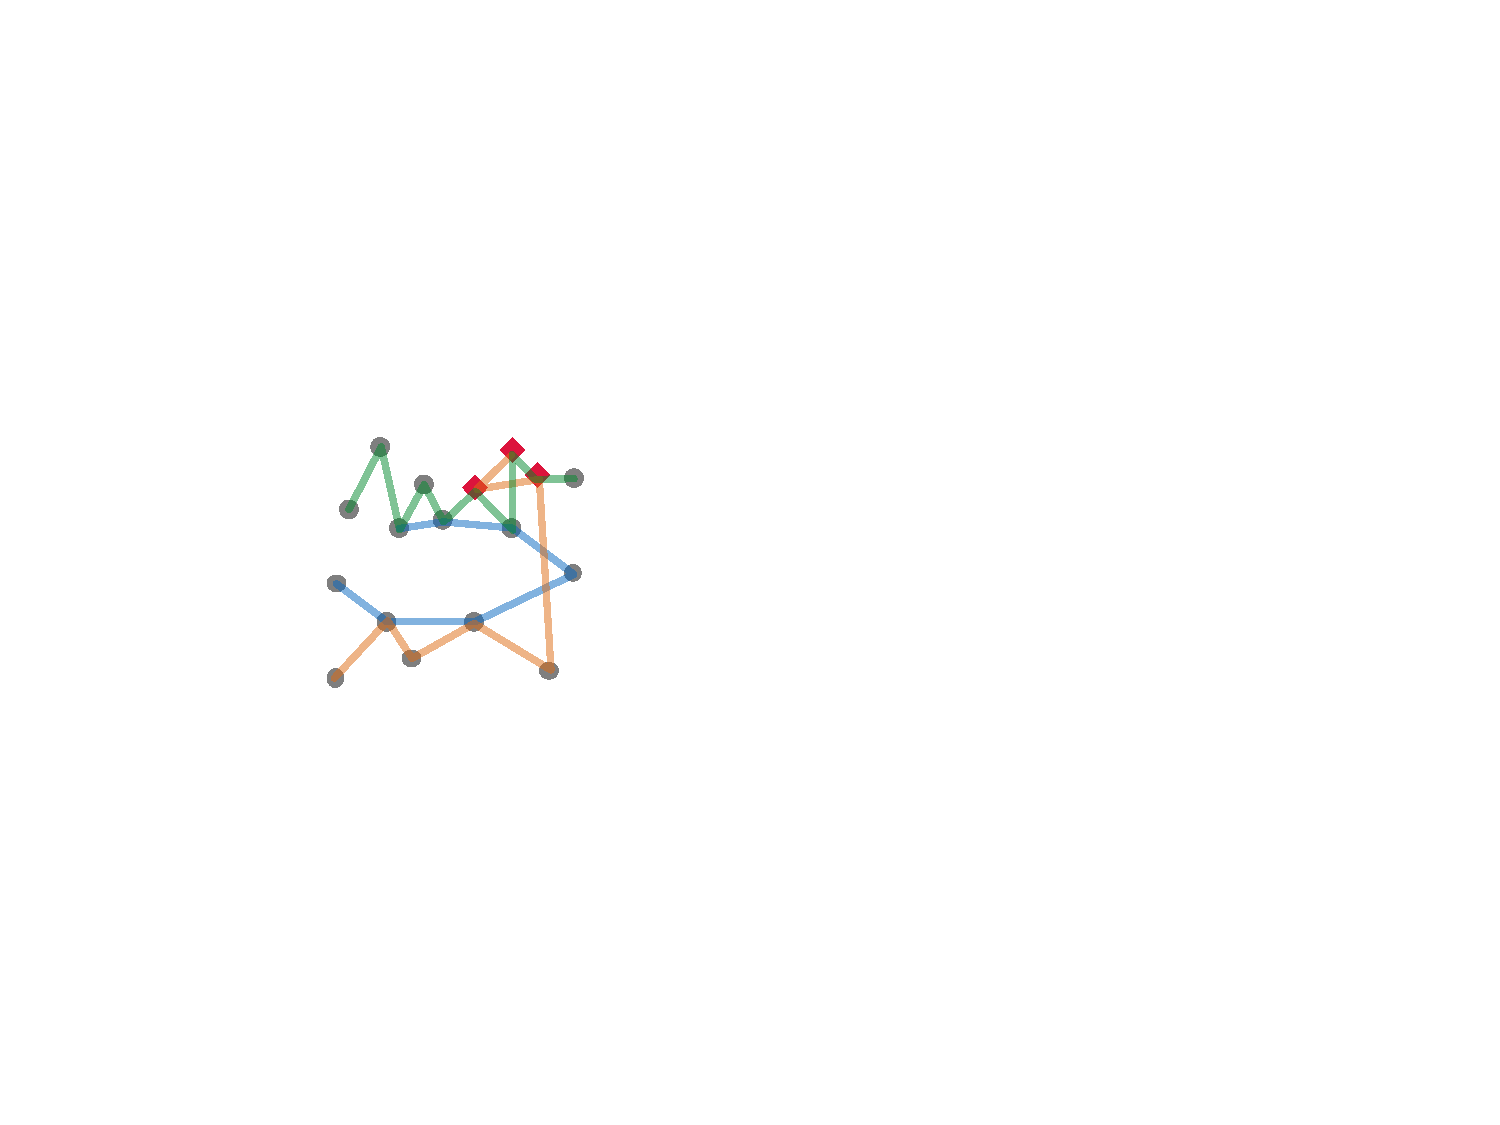
\includegraphics[width=.35\columnwidth]{figure4a}}
%	\hfill	
%	\subcaptionbox{Shared events are duplicated in both green and orange sets.\label{fig:layering-2}}[.478\columnwidth]
%	{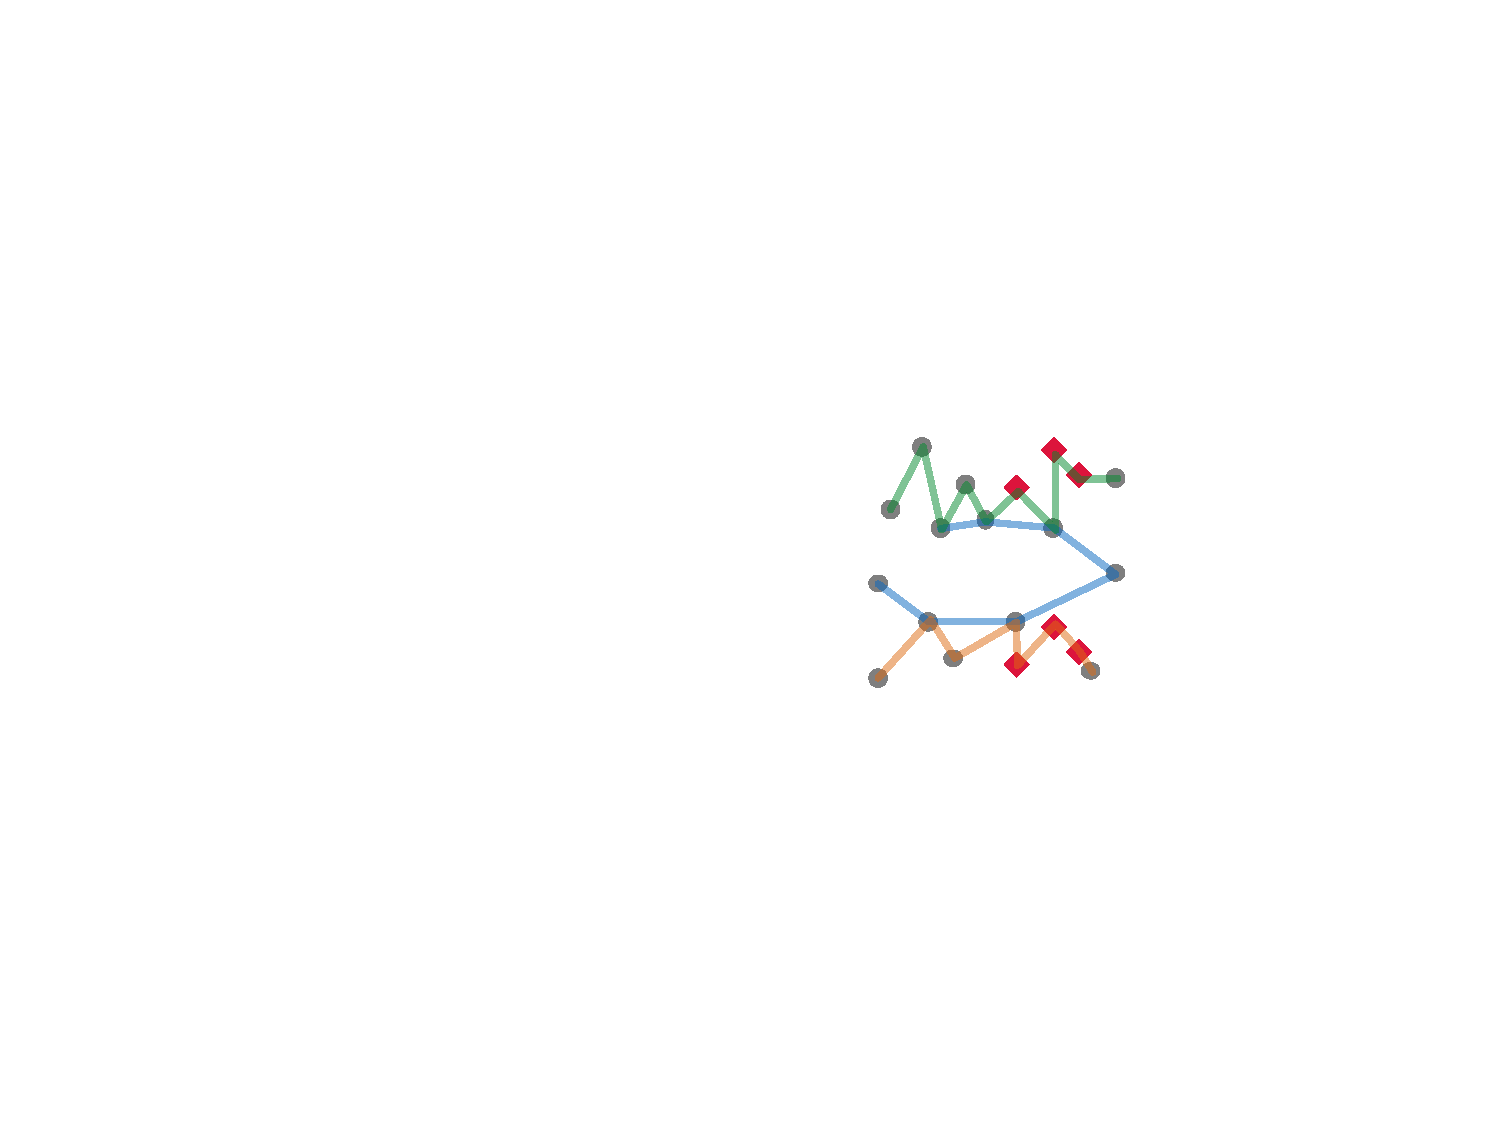
\includegraphics[width=.35\columnwidth]{figure4b}}
%	\caption{Visualization of shared events (red squares) between two non-neighboring sets.}
%	\label{fig:layering-compare}
%\end{figure}
%
%In subsequent sections, we discuss the detail of the set visualization algorithm, which consists of two main steps: generating set shapes, and then coloring them.
%
%\subsubsection{Shape Generation}
%This algorithm takes as input a list of bounding-boxes of the set's events, and generates a closed-curve containing all these boxes. 
%
%\begin{figure}[!htb]
%	\centering
%	\subcaptionbox{The original rectilinear shape generated by a scan-line algorithm.\label{fig:shape1}} 
%	{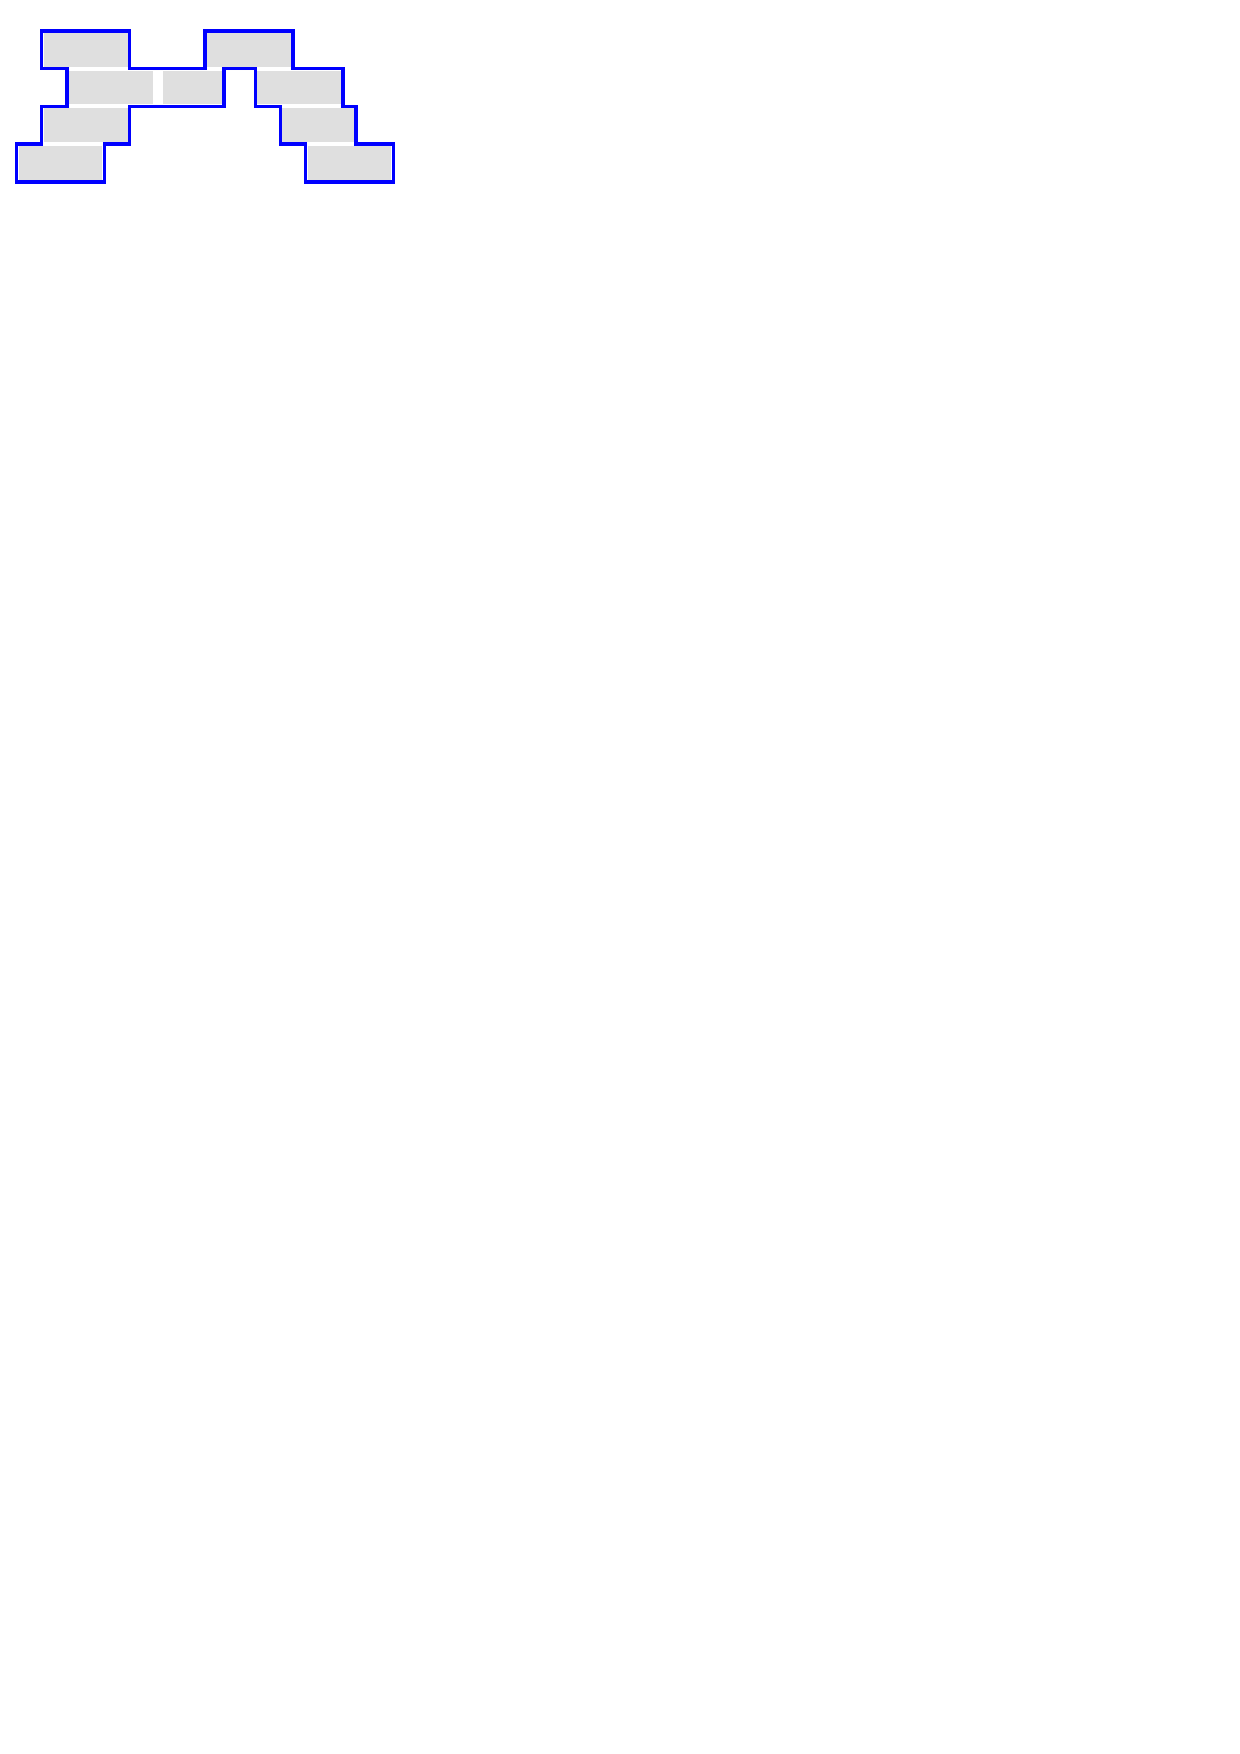
\includegraphics[width=.47\columnwidth]{figure5a}}
%	\hfill
%	\subcaptionbox{The simplified shape by flattening and removing jags (red eclipse).\label{fig:shape2}}
%	{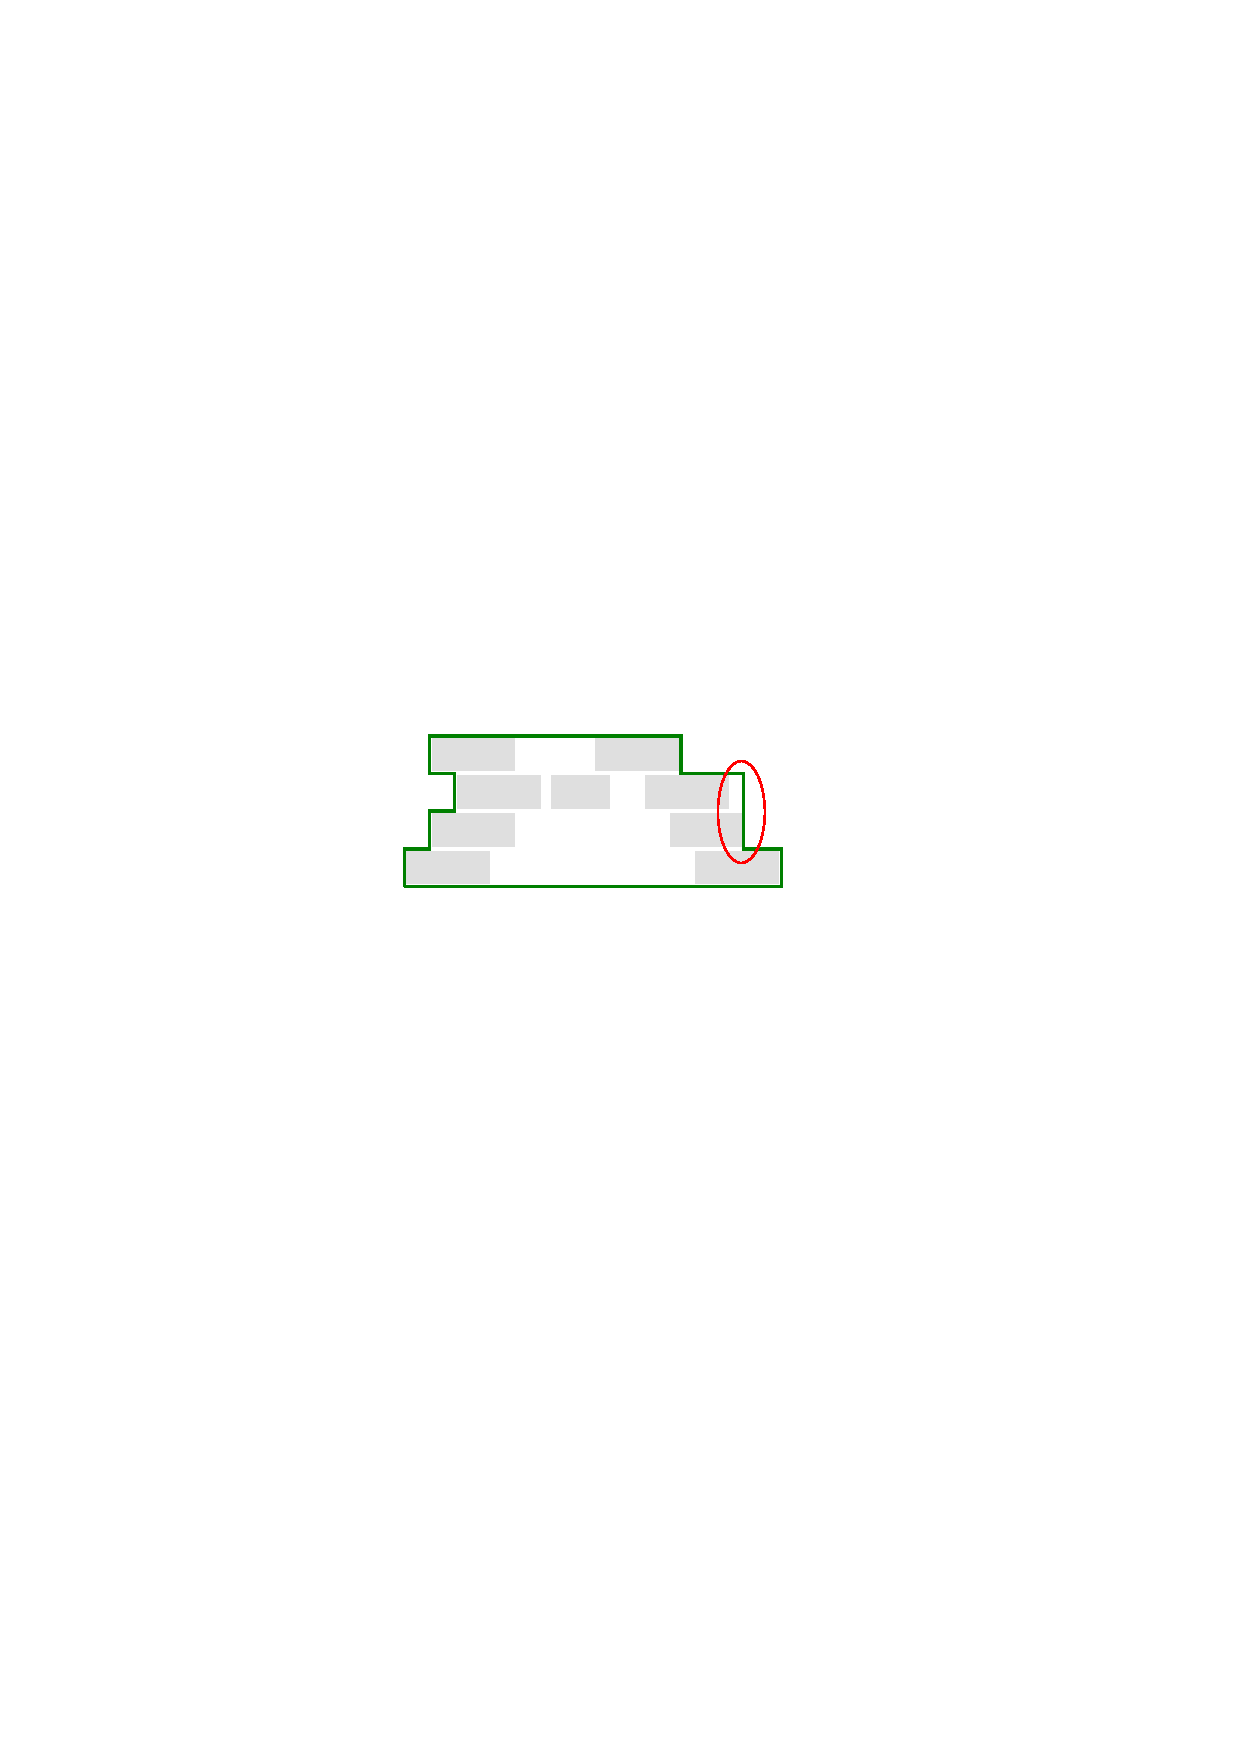
\includegraphics[width=.47\columnwidth]{figure5b}}
%	\caption{Rectilinear shape generation.}
%	\label{fig:shape}
%\end{figure}
%
%\begin{figure}[!htb]
%	\centering
%	\subcaptionbox{Vertical segments $e_2$ and $e_3$ are converted to diagonal ones (dashed lines).\label{fig:generation1}}
%	{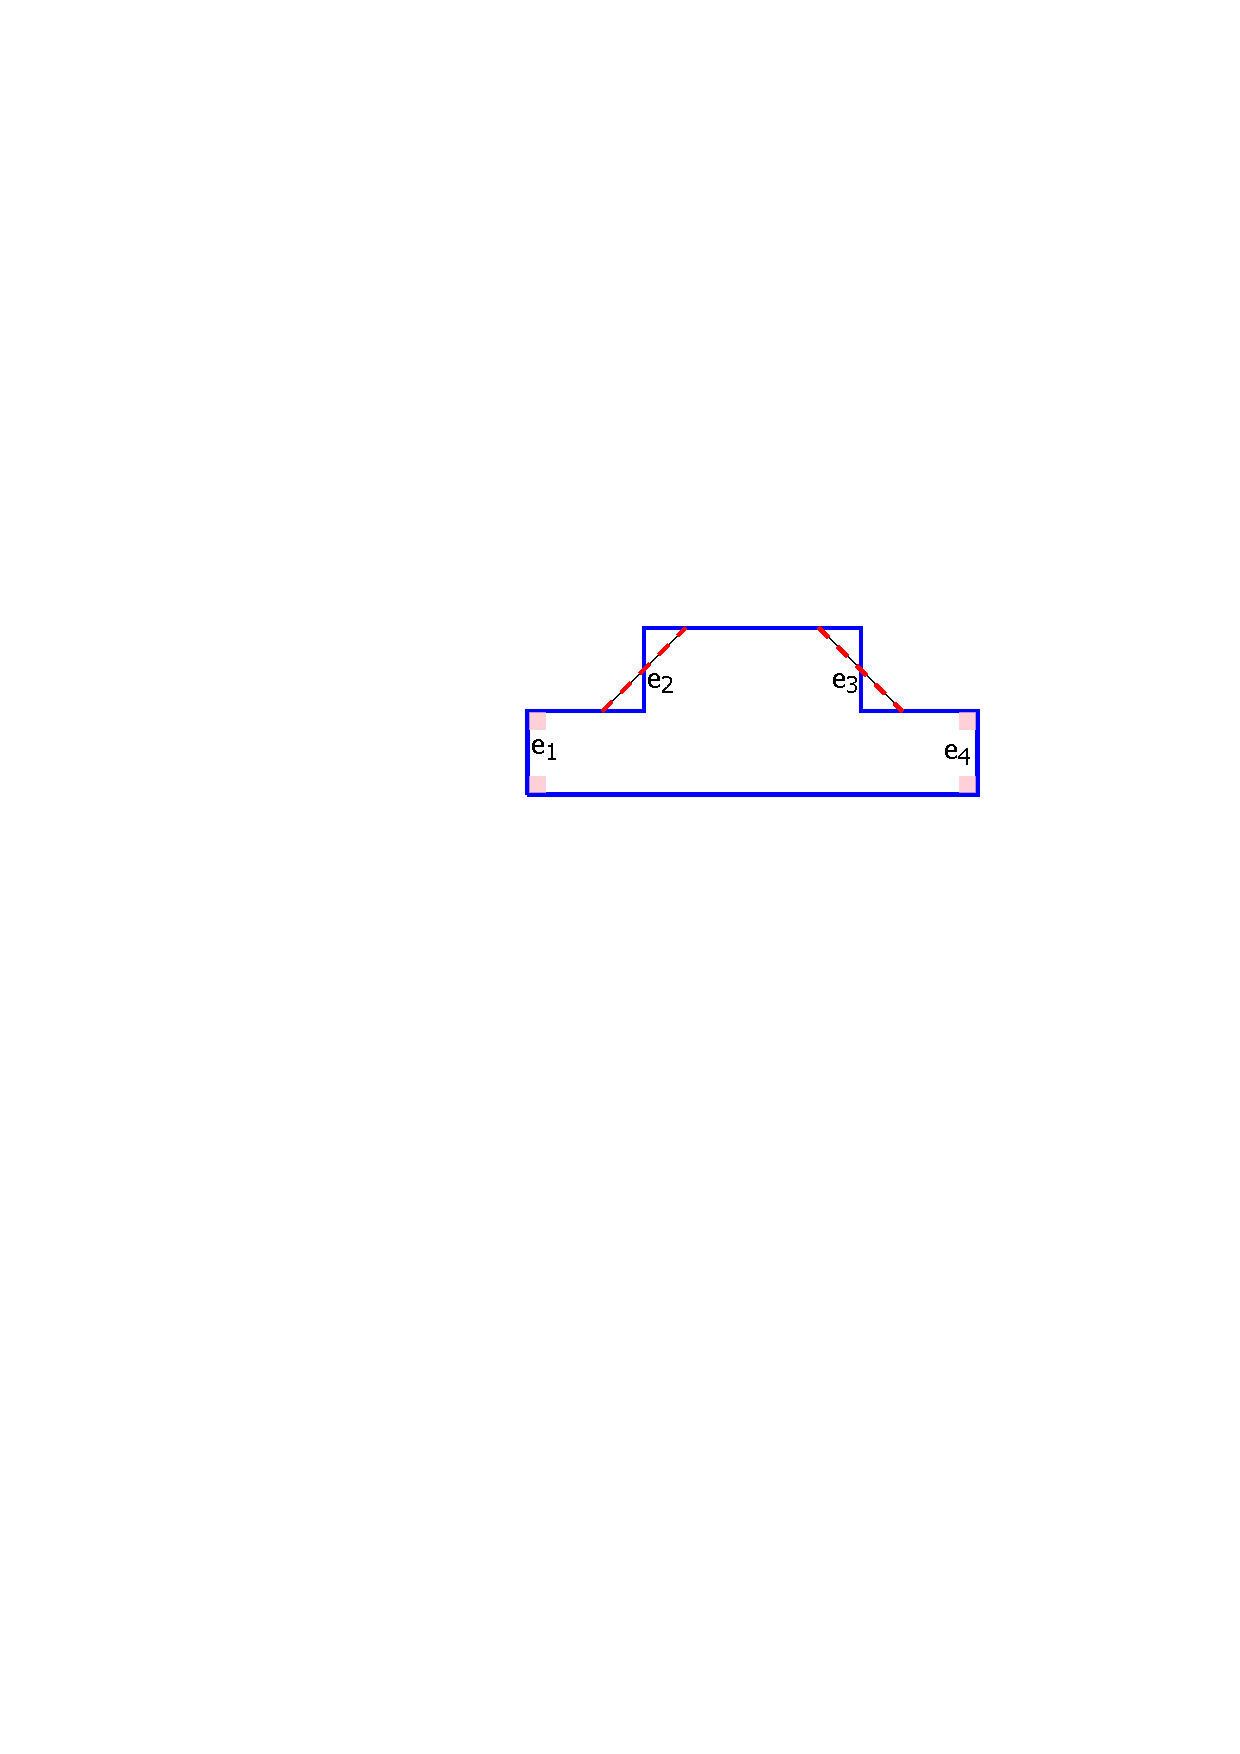
\includegraphics[width=.47\columnwidth]{figure6a}}
%	\hfill
%	\subcaptionbox{Squared corners are replaced by quadrant arcs. $e_2$ and $e_3$ are further smoothened by B\'{e}zier curves.\label{fig:generation2}}
%	{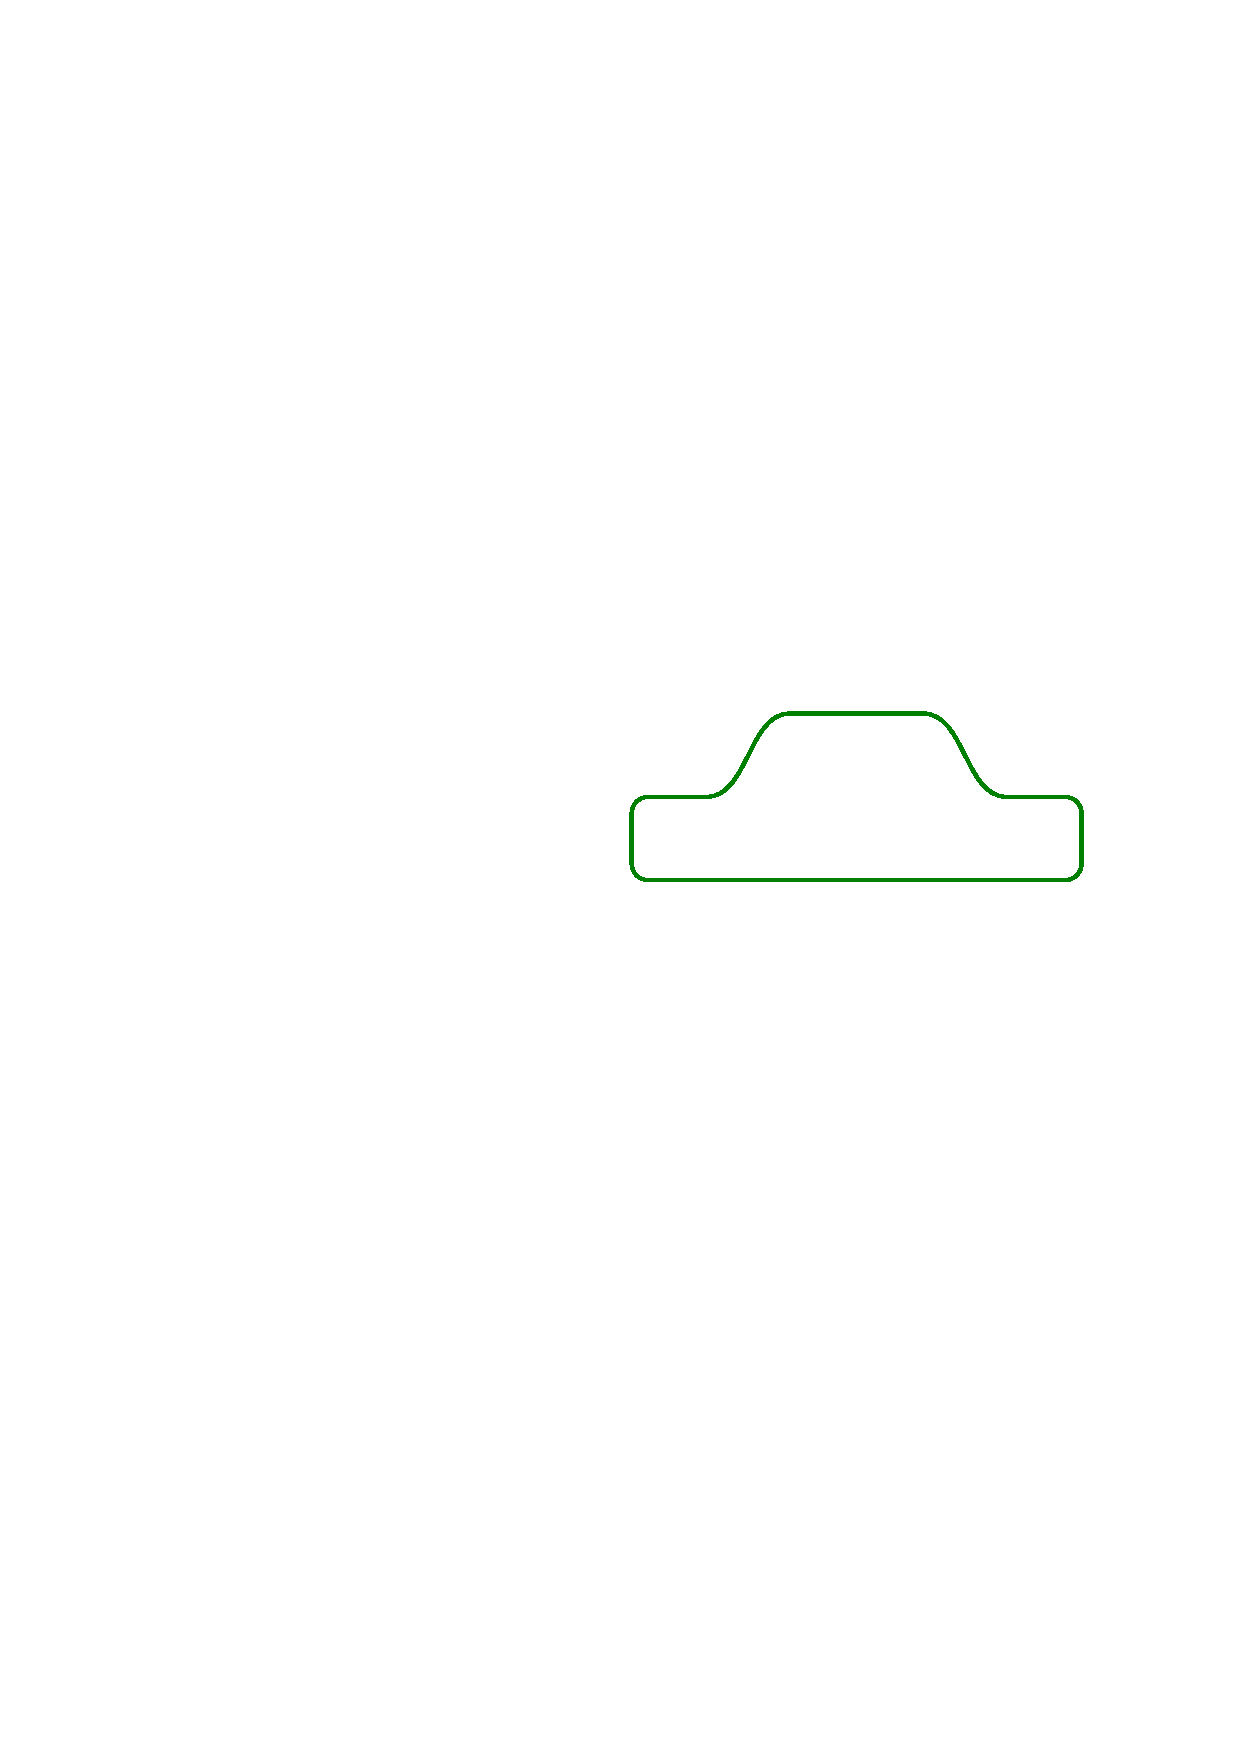
\includegraphics[width=.47\columnwidth]{figure6b}}
%	\caption{Shape smoothening by reducing the degree of line bends.}
%	\label{fig:generation}
%\end{figure}
%
%\subsubsection{Set Coloring}
%Each set is filled with a color selected from Qualitative Set 2 of ColorBrewer~\cite{Harrower2003} to make them easily distinguishable. And the background of the intersection between two sets is shown as the color transitioned between the two set colors (Figure~\ref{fig:gradient}).
%
%\begin{figure}[!htb]
%	\centering
%	\subcaptionbox{Intersection shown as a single color gradient.\label{fig:gradient1}}
%	{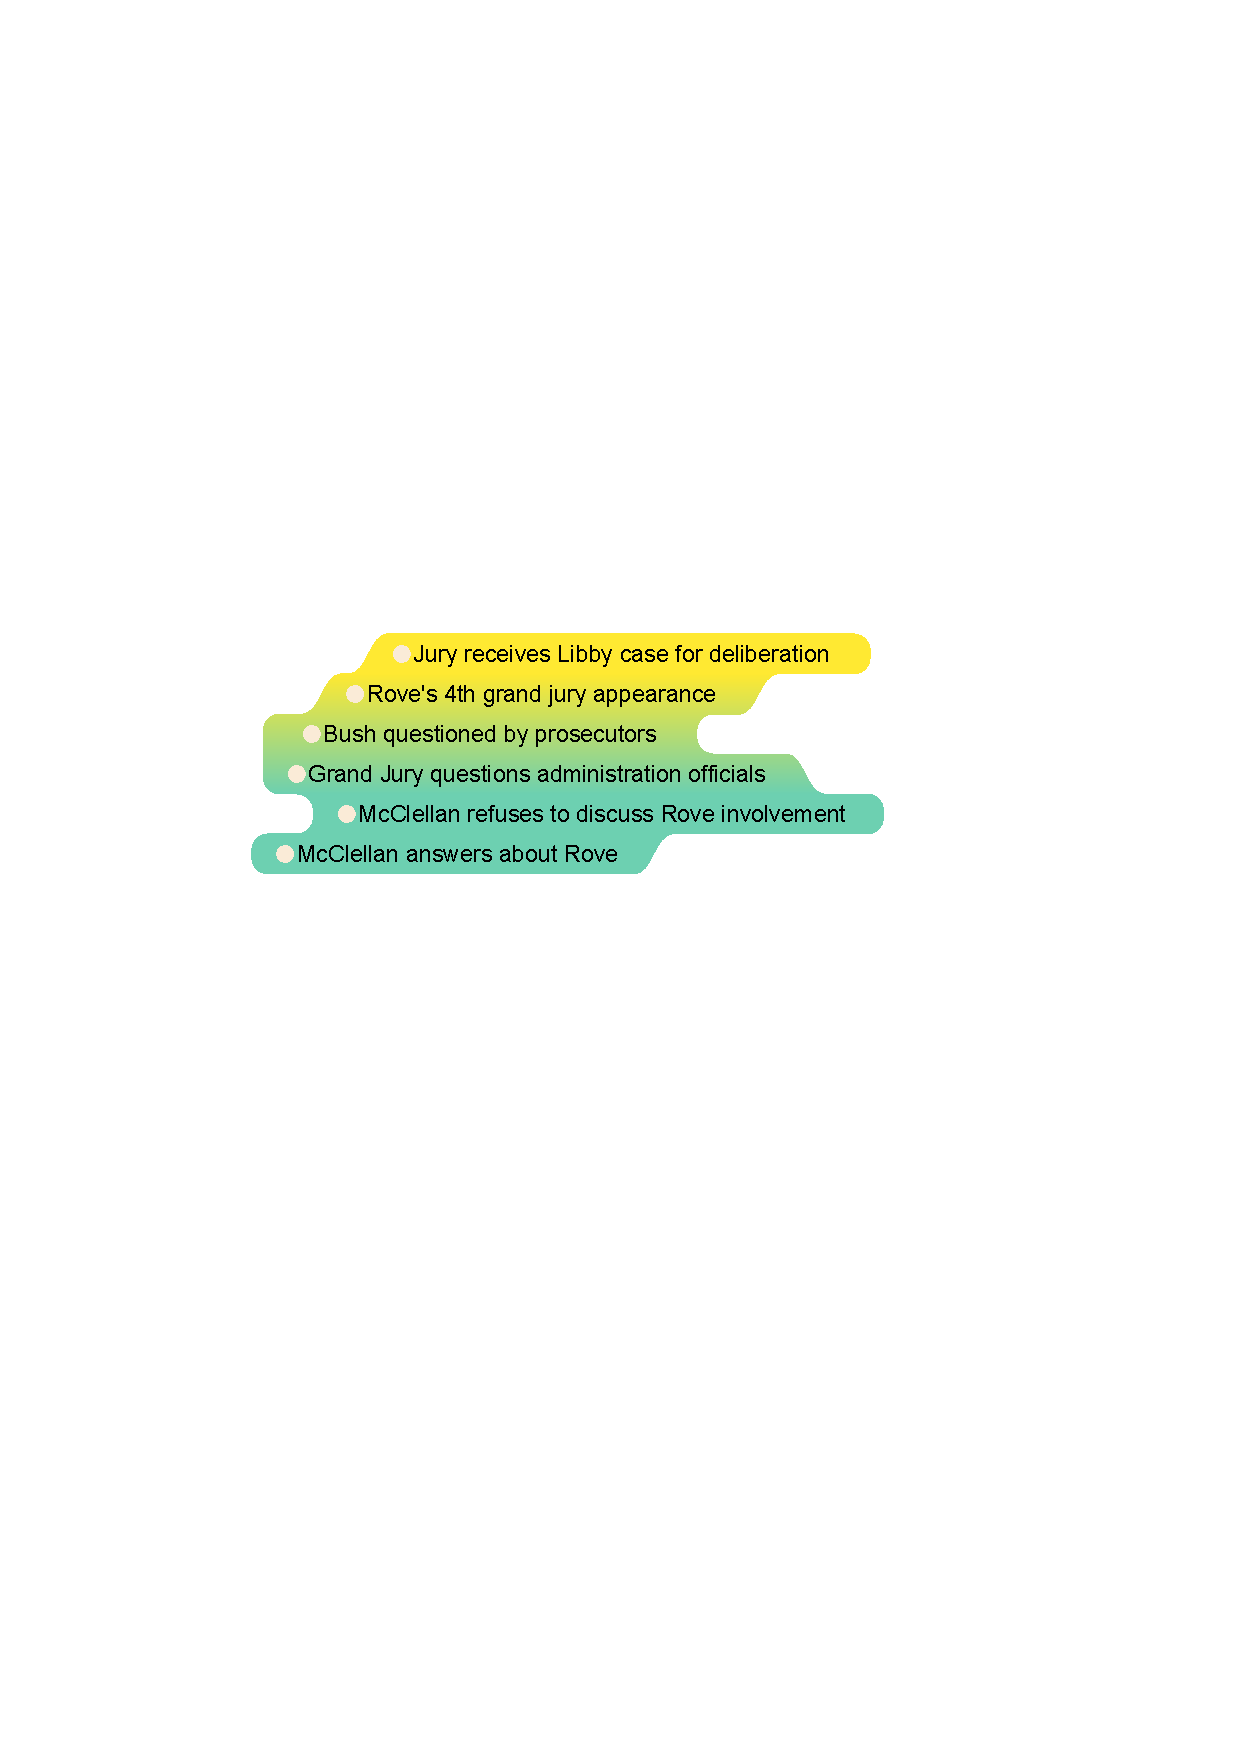
\includegraphics[width=0.47\columnwidth]{figure7a}}
%	\hfill
%	\subcaptionbox{Intersection shown as multiple color gradients.\label{fig:gradient2}}
%	{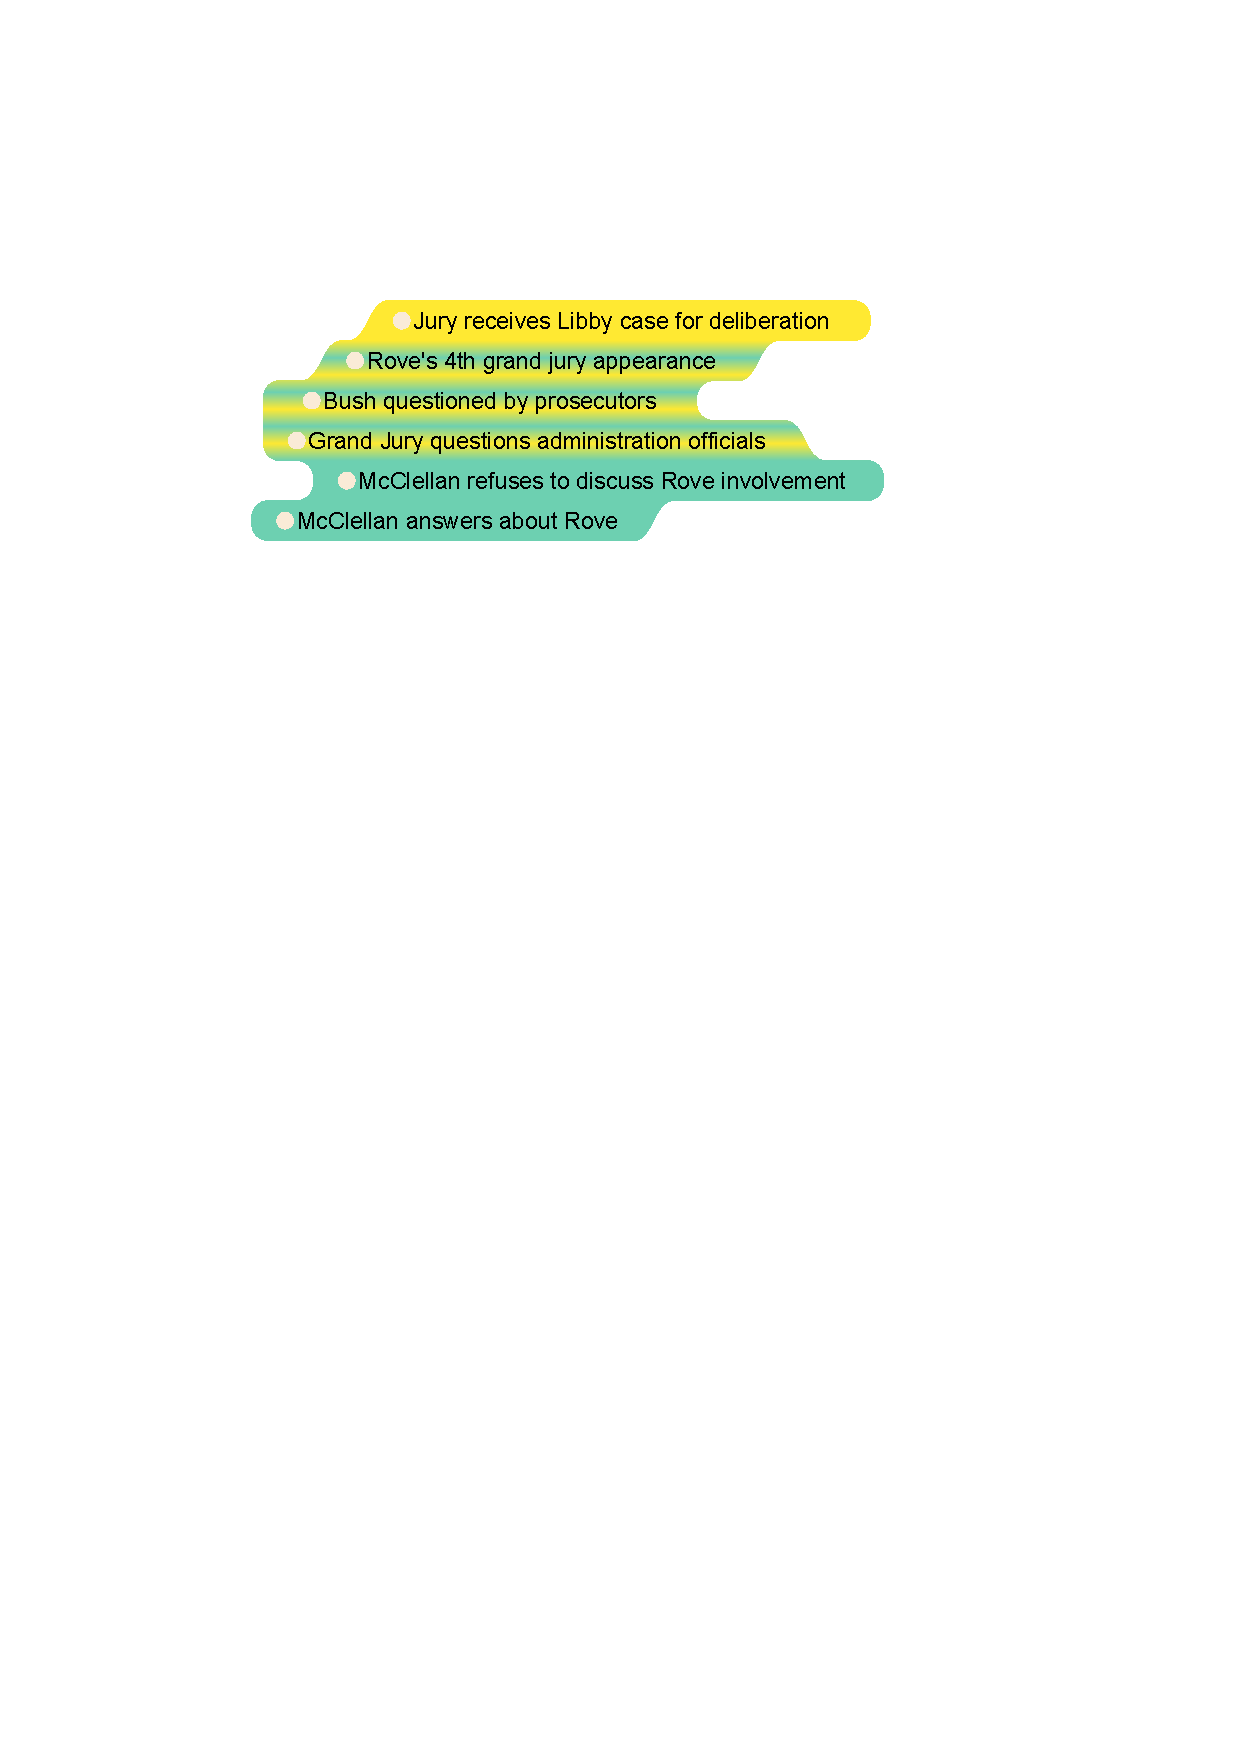
\includegraphics[width=0.47\columnwidth]{figure7b}}
%	\caption{Color gradient technique to encode set intersection. The gradient area shows three shared events between the yellow and green sets.}
%	\label{fig:gradient}
%\end{figure}
%
%\subsubsection{Multiple-set Events}
%Four design options are proposed to visualize the full set memberships of events.
%
%\begin{figure}[!htb]
%	\centering
%	\subcaptionbox{Each circle represents a set.\label{fig:eventmembership1}}[.22\columnwidth]{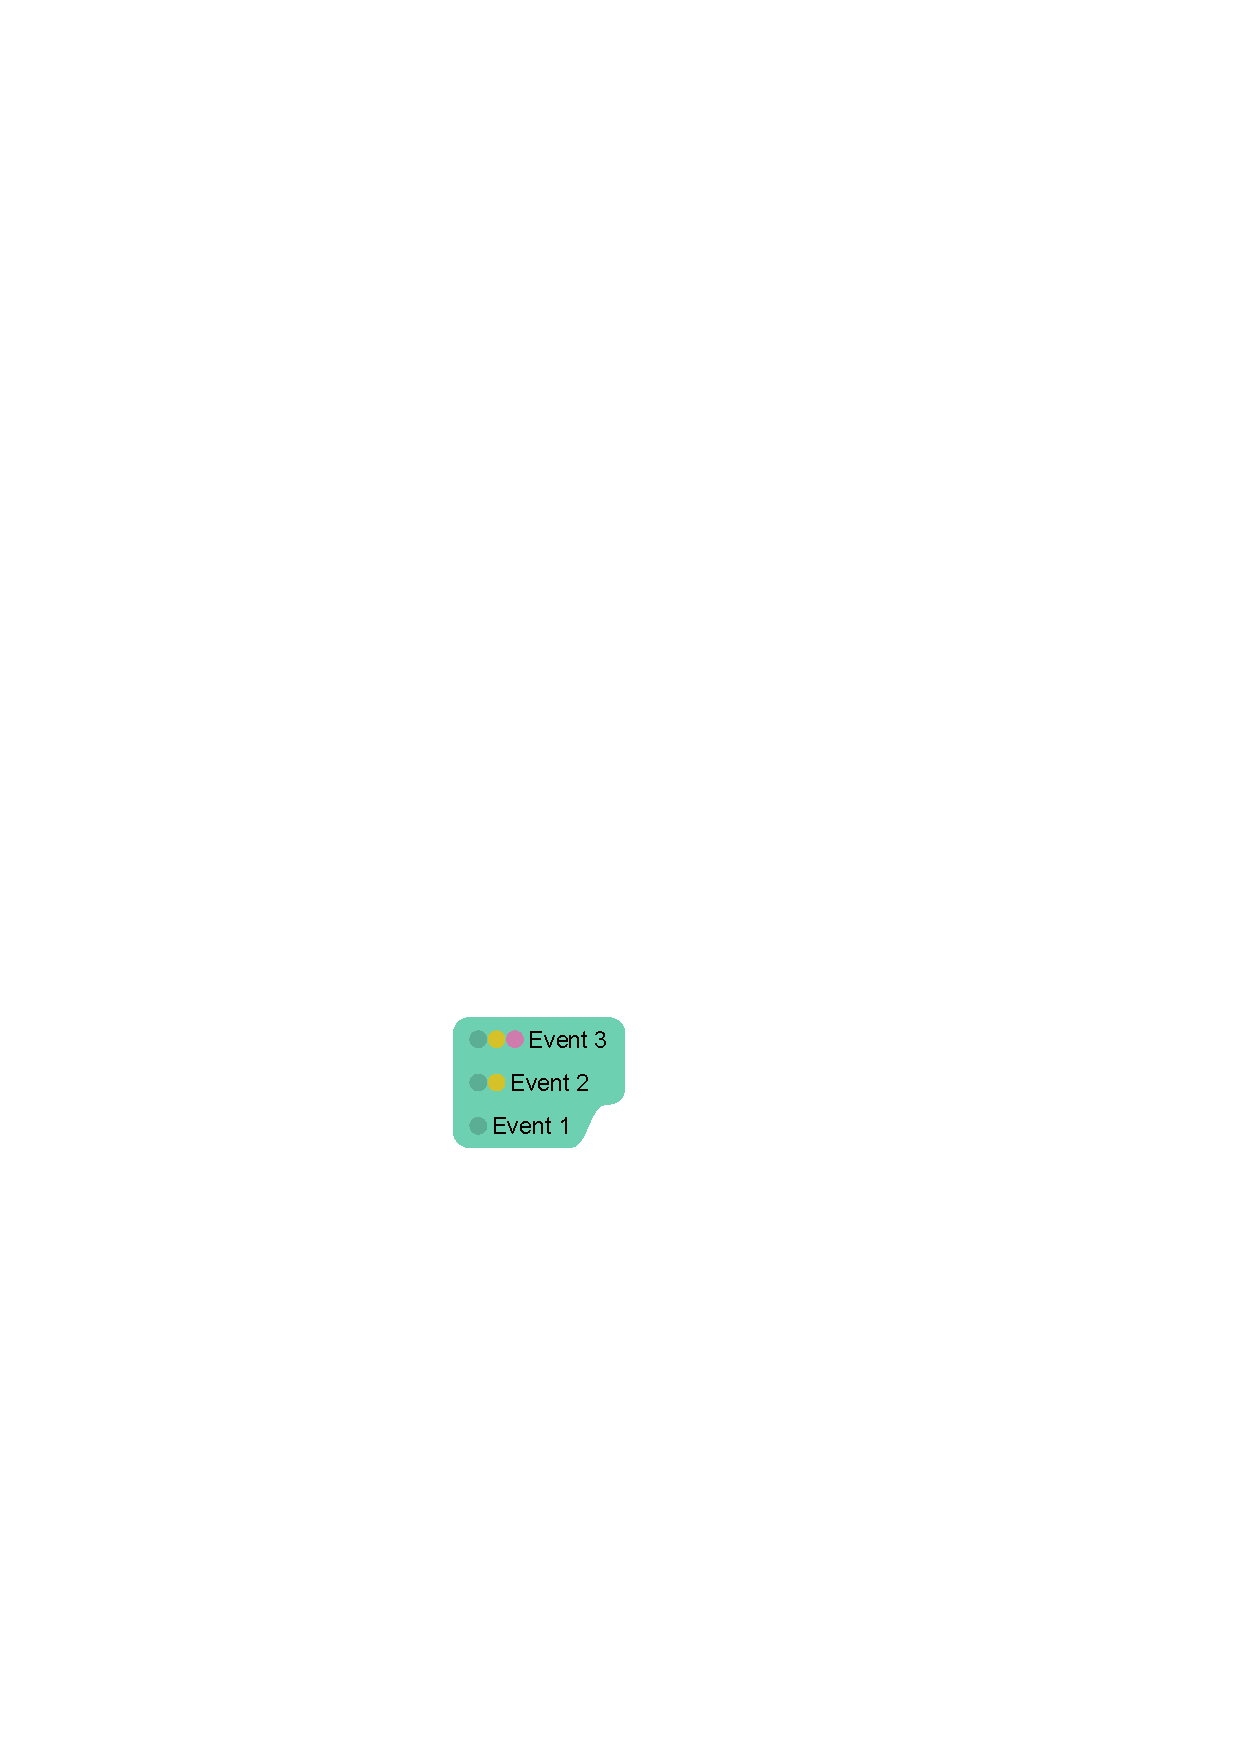
\includegraphics[height=.18\columnwidth]{figure8a}}
%	\hfill
%	\subcaptionbox{Each ring represents a set.\label{fig:eventmembership2}}[.22\columnwidth]{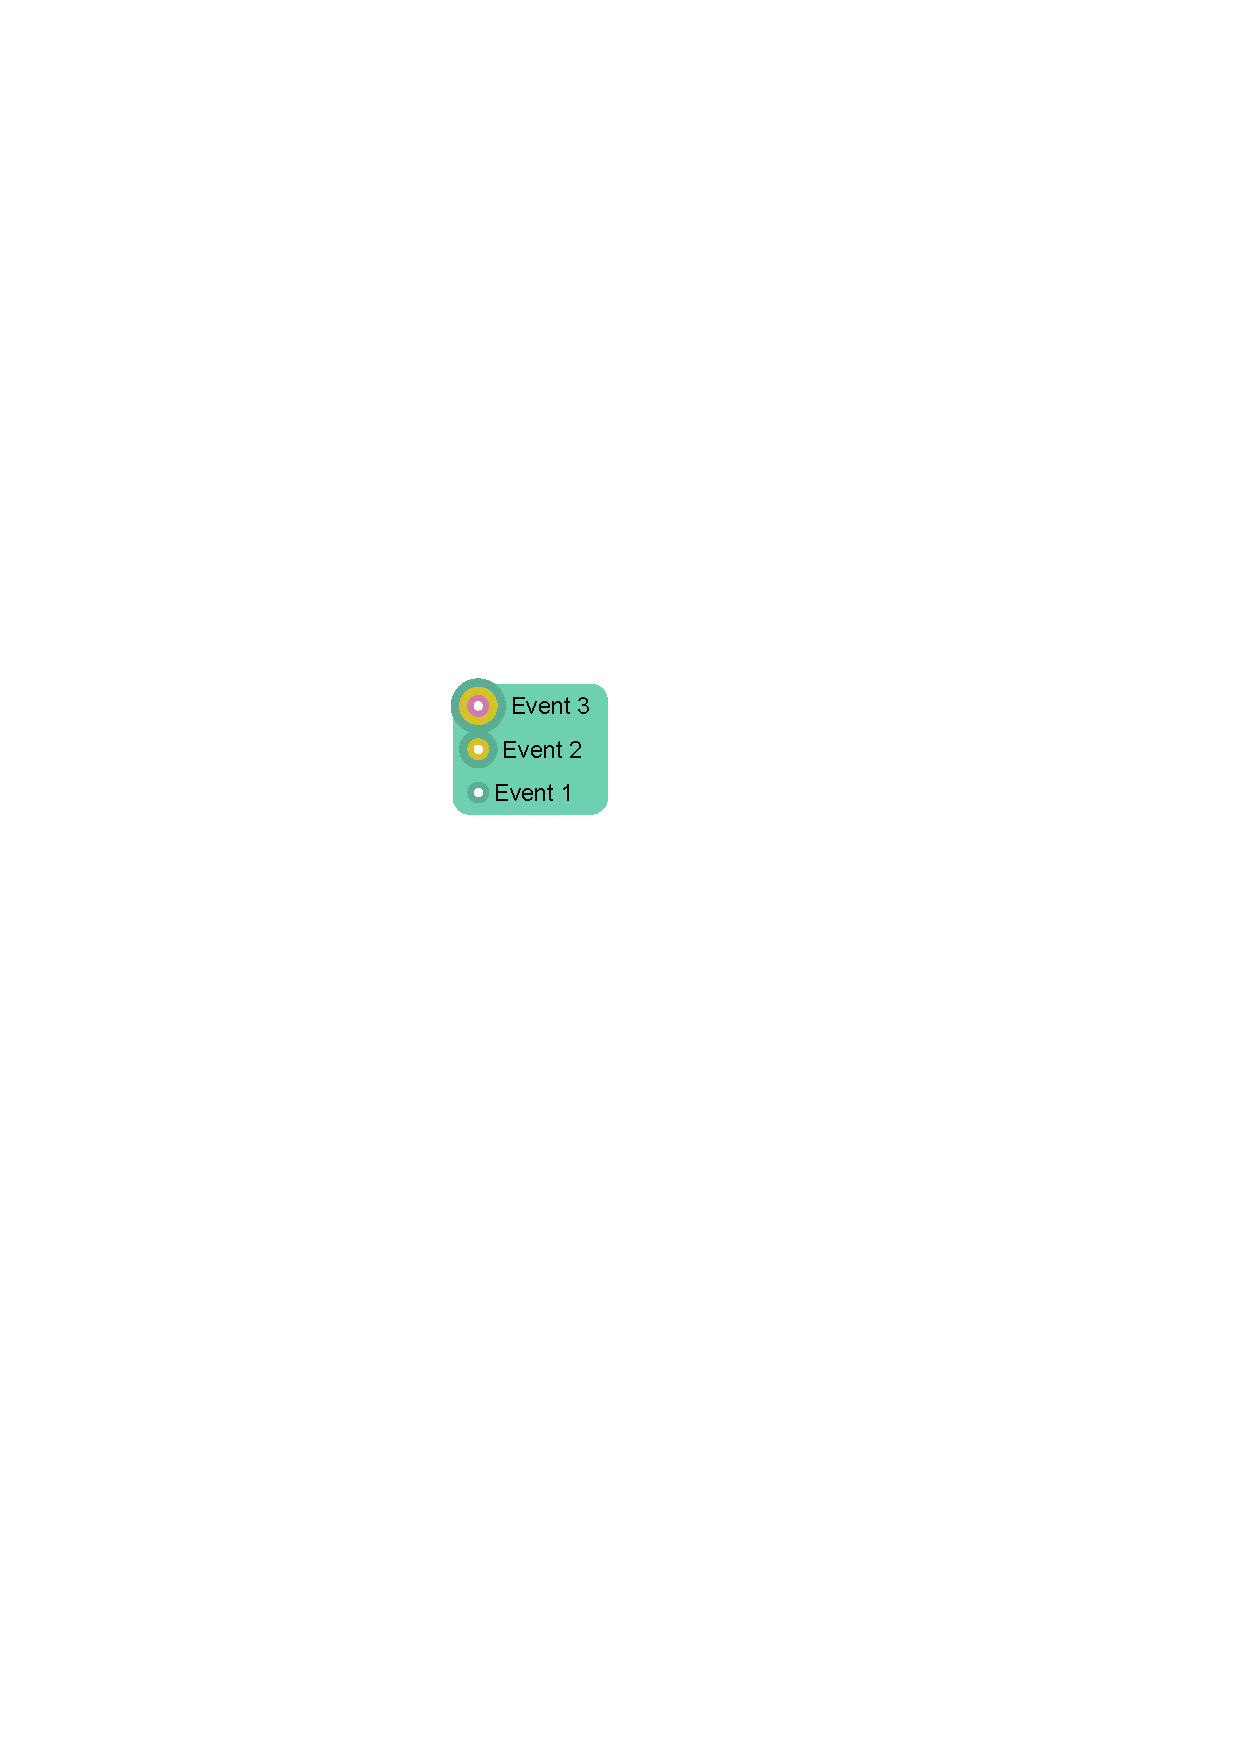
\includegraphics[height=.19\columnwidth]{figure8b}}
%	\hfill
%	\subcaptionbox{Vertical gradient: each color represents a set.\label{fig:eventmembership3}}[.22\columnwidth]{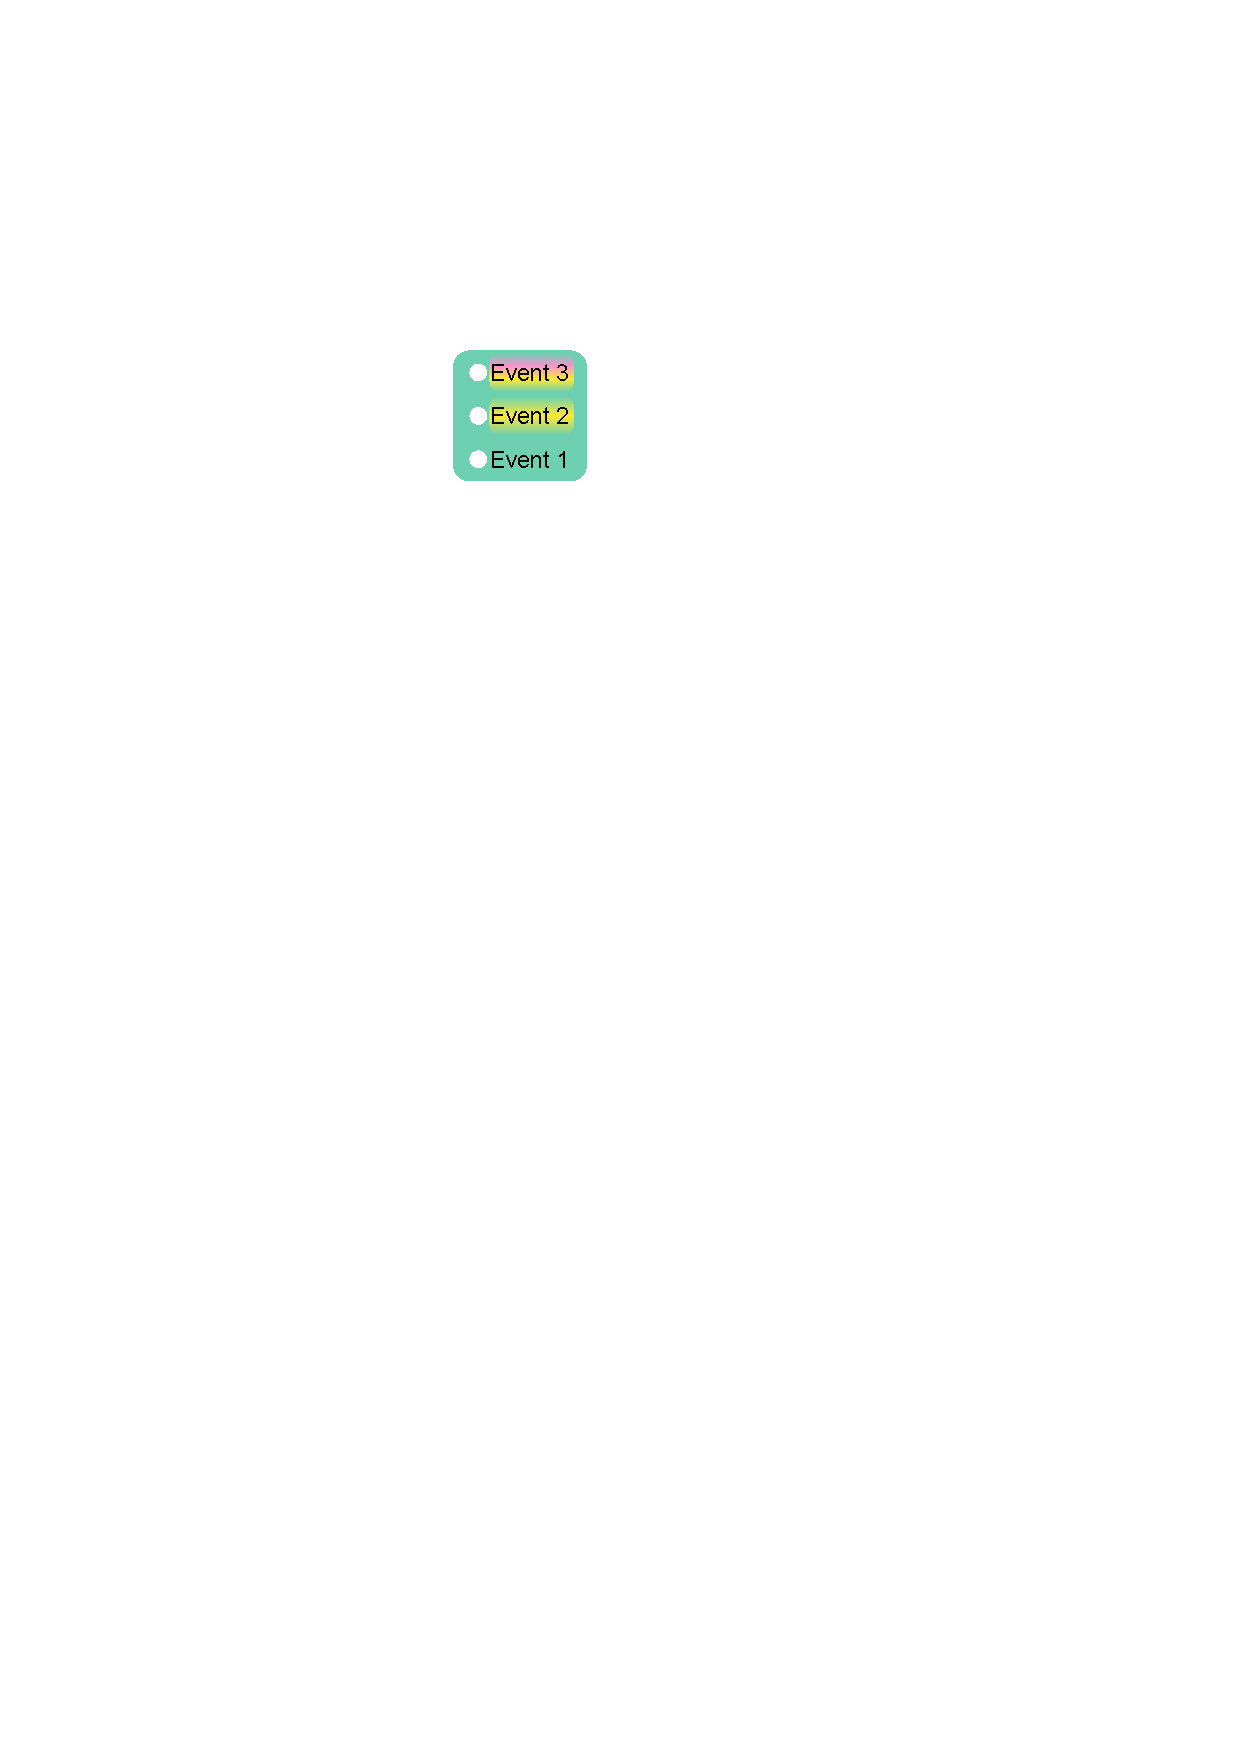
\includegraphics[height=.18\columnwidth]{figure8c}}
%	\hfill
%	\subcaptionbox{Horizontal gradient: each color represents a set.\label{fig:eventmembership4}}[.22\columnwidth]{\includegraphics[height=.18\columnwidth]{figure8d}}
%	\caption{Visual representation of multiple-set events. Event 1 is single-set (green). Event 2 is double-set (green, yellow). Event 3 is triple-set (green, yellow, pink).}
%	\label{fig:eventmembership}
%\end{figure}
%
%Putting it all together, Figure~\ref{fig:sl-overview} shows an example of a complete SchemaLine. The algorithm to produce this visualization is described in Section~\ref{sec:sl-algorithm}.
%
%\begin{figure}[!htb]
%	\centering
%	\includegraphics[width=\linewidth]{figure1}
%	\caption{TimeSets visualization of the CIA leak case. The timeline contains events that happened from 2002 to 2007, each includes a timestamp, a label, and topics such as ``White House''. Events are positioned along the horizontal time axis based on their temporal values, and vertically grouped by colored topics (see the color legend in the bottom right corner).}
%	\label{fig:ts-overview}
%\end{figure}
%
%\subsection{Interaction}
%Describe interaction including zoom, pan, mouse hover, filter.
%
%\section{Layout}
%\label{sec:ts-algorithm}
%
%\subsection{Sets Ordering}
%The same as the schema ordering algorithm in SchemaLine
%
%\subsection{Layer Layout}
%This algorithm positions all the events within a layer. We propose two algorithms: one is optimized to display as much information as possible (\emph{completeness}), and the other one is optimized for the convenience to follow events (\emph{traceability}).
%
%\begin{figure}[!htb]
%	\centering
%	\subcaptionbox{Completeness algorithm: $\theta=1$, \\$\gamma=5/3$.}{\includegraphics[width=.47\linewidth]{figure9a}}
%	\hfill
%	\subcaptionbox{Traceability algorithm ($t_{min}=0.5$, $r_{max}=1$): $\theta=6/7$, $\gamma=2/3$.}{\includegraphics[width=.47\linewidth]{figure9b}}
%	\caption{Layer layout algorithms. Each rectangle represents an event. The line connecting centers of rectangles illustrates the  traceability.}
%	\label{fig:traceability}
%\end{figure}
%
%\subsection{Layers Compacting}
%Compact layers together leaving no gap rows among layers.
%
%\begin{figure}[!htb]
%	\centering
%	\subcaptionbox{Before: consumed height = 6 rows.}{\includegraphics[width=.44\columnwidth]{figure10a}}
%	\hfill
%	\subcaptionbox{After: consumed height = 3 rows.}{\includegraphics[width=.44\columnwidth]{figure10b}}
%	\caption{Layers compacting.}
%	\label{fig:compacting}
%\end{figure}
%
%\subsection{Layers Balancing}
%This last step ensures that all layers have similar levels of detail; i.e., avoiding layers with many complete events and other layers with many aggregated events.
%
%\begin{figure}[!htb]
%	\centering
%	\subcaptionbox{Before: $\theta_{green}=0.25$, $\theta_{yellow}=1$.}{\label{fig:balancing1}\includegraphics[width=.44\columnwidth]{figure11a}}
%	\hfill
%	\subcaptionbox{After: $\theta_{green}=\theta_{yellow}=0.5$.}{\label{fig:balancing2}\includegraphics[width=.44\columnwidth]{figure11b}}
%	\caption{Layers balancing.}
%	\label{fig:balancing}
%\end{figure}
%
%\section{Evaluation}
%\begin{itemize}
%	\item Goal: compare task performance between TimeSets and a relevant state-of-the-art visualization technique (KelpFusion)
%	\item Method: lab controlled experiment, within-subject
%	\item Task: 5 different tasks related to temporal and set relations using 4 generated datasets
%	\item Participants: 30, each answers 2 x 5 x 4 = 40 questions
%	\item Procedure:  introduction $\rightarrow$ practice $\rightarrow$ main task $\rightarrow$ subjective questionnaire 
%	\item Report: RM-ANOVA significant tests to analyze performance data and Fisher's exact tests to analyze user ratings
%\end{itemize}
%
%\section{Case Study 1: Publication Data}
%Shows an application of TimeSets to publication data of 200 articles and 8 sets. Discuss interesting findings with TimeSets.
%
%\begin{figure}[!htb]
%	\centering
%	\includegraphics[width=\linewidth]{figure13}
%	\caption{TimeSets visualization of publication data. It shows 200 articles with the most citations in the IEEE InfoVis conference from 1995 to 2013. These articles are categorized based on their concepts (see the legend in the top left hand corner).}
%	\label{fig:citations}
%\end{figure}
%
%\section{Case Study 2: VAST Challenge 2014}
%Shows an application of TimeSets to intelligence analysis. TimeSets is used to show both tweets (\note{this is the color blending version of TimeSets, not color gradient -- should we describe the color blending one?}, Figure~\ref{fig:savi}) and findings (\note{missing figure -- currently, findings are shown as a node-link diagram})
%
%\begin{figure}[!htb]
%	\centering
%	\includegraphics[width=\linewidth]{HQ-savi}
%	\caption{}
%	\label{fig:savi}
%\end{figure}
